%% LyX 2.0.1 created this file.  For more info, see http://www.lyx.org/.
%% Do not edit unless you really know what you are doing.
\documentclass[10pt, conference, letterpaper]{IEEEtran}
\usepackage[T1]{fontenc}
\usepackage[latin9]{inputenc}
%\usepackage{babel}
\usepackage{color}



% *** ALGORITHM PACKAGES ***
\usepackage{algorithm}
\usepackage{algorithmicx}
\usepackage{algpseudocode}

\renewcommand{\algorithmicrequire}{\textbf{Input:}} % Use Input in the format of Algorithm
\renewcommand{\algorithmicensure}{\textbf{Output:}} % Use Output in the format of Algorithm


\usepackage{amsthm}
\usepackage{amsmath}
\usepackage{amssymb}
\usepackage{float}
\usepackage{caption}
\usepackage{graphicx}
\usepackage{subcaption}
%\usepackage{subfigure}
\usepackage{epsfig}
\usepackage{balance}
\usepackage{multirow}
\usepackage{url}
\usepackage{color}

%\usepackage[unicode=true,
% bookmarks=true,bookmarksnumbered=true,bookmarksopen=true,bookmarksopenlevel=1,
% breaklinks=false,pdfborder={0 0 0},backref=false,colorlinks=false]
% {hyperref}
%\hypersetup{pdftitle={Your Title},
% pdfauthor={Your Name},
% pdfpagelayout=OneColumn,pdfnewwindow=true,pdfstartview=XYZ,plainpages=false}

%XXX~Longo~XXX Start Add%
\usepackage{enumitem}
\setenumerate[1]{itemsep=1pt,partopsep=0pt,topsep=5pt}
\setitemize[1]{itemsep=1pt,partopsep=0pt,topsep=5pt}
\setdescription{itemsep=1pt,partopsep=0pt,topsep=5pt}

\captionsetup{aboveskip=0pt,belowskip=-8pt}
\captionsetup[figure]{font=footnotesize,labelfont=footnotesize}
\captionsetup[subfigure]{font=footnotesize,labelfont=footnotesize}

\addtolength{\topmargin}{0.3in}
\setlength{\columnsep}{0.23in}

%XXX~Longo~XXX End Add%

\makeatletter


%%%%%%%%%%%%%%%%%%%%%%%%%%%%%% LyX specific LaTeX commands.
%% Because html converters don't know tabularnewline
\providecommand{\tabularnewline}{\\}
%% A simple dot to overcome graphicx limitations
\newcommand{\lyxdot}{.}



%%%%%%%%%%%%%%%%%%%%%%%%%%%%%% Textclass specific LaTeX commands.
\theoremstyle{plain}
\newtheorem{thm}{\protect\theoremname}
\theoremstyle{definition}
\newtheorem{defn}[thm]{\protect\definitionname}
\theoremstyle{plain}
\newtheorem{lem}[thm]{\protect\lemmaname}

%%%%%%%%%%%%%%%%%%%%%%%%%%%%%% User specified LaTeX commands.
\@ifundefined{definecolor}{\usepackage{color}}{}
\@ifundefined{definecolor}{\usepackage{color}}{}
% for subfigures/subtables



\providecommand{\definitionname}{Definition}
\providecommand{\examplename}{Example}
\providecommand{\lemmaname}{Lemma}
\providecommand{\theoremname}{Theorem}
\providecommand{\theoremname}{Problem}



% *** GRAPHICS RELATED PACKAGES ***
\graphicspath{{pix/}}






% *** Page scaling Setup ***
\renewcommand{\baselinestretch}{0.96}



\makeatother




% *** PAGE # ***
\pagenumbering{arabic}
\pagestyle{plain}

% *** Theorem ***
%\newcounter{lemma}
%\newcounter{definition}
%\newcounter{problem}
%\newcounter{theorem}
%\newcounter{corollary}
\newcounter{proposition}
%
\newtheorem{prop}[proposition]{Proposition}
%
\newtheorem{prob}{Problem}

%\newtheorem{defi}{Definition}

\DeclareMathOperator*{\argmax}{arg\,max}


\begin{document}

\title{\global\long\def\lcm{\textrm{lcm}}
 \global\long\def\gcd{\textrm{gcd}}
Optimal Trajectory Planning of Drones \\ for 3D Mobile Sensing}

% Modeling Online Social Homophily in Offline Geographical Communities

%\author{Paper ID: 1570300720}
\author{Anonymous}

\maketitle

\begin{abstract}
Mobile sensing is challenging in 3D space, as there are many inaccessible places where people rarely venture. Unmanned aerial vehicle (UAV), commonly known as drone, has greatly extended the scope of mobile sensing in 3D space, and pushed forward a variety of 3D mobile sensing applications, such as aerial photo- or video-graphy, 3D wireless signal survey, air quality monitoring. However, the short battery life of drones has largely restricted the wide adoption of these applications.
To maximally expand the sensing scope of the drone, in this paper, we study the trajectory planning problem for optimizing its flight route in 3D space, given its limited battery life.
We first divide the target 3D space into a grid of observation locations formed by multiple 2D grids. By extending the concept of dominating set, we formulate the problem as finding the minimum dominating path in the grid to cover the sensing scope in 3D space with the minimum trajectory, and then select necessary critical observation locations within the trajectory for the drone to hover and perform the measurement.
Experimental results show that the proposed algorithm takes 32\% less time to complete sensing the given space, and during the battery life it can cover 19\% more sensing scope, than existing solutions.
%XXX related work
%XXX 2d mobile base station
%XXX 3d map using vision technique
\end{abstract}

\section{Introduction}~\label{sec:intro}

%1. ·É»úÓŠÓúܶ࣬Ö÷Òª»¹ÊÇÊÕŒ¯ÊýŸÝ£¬·ÉµœÈËÀàÎÞ·šŽ¥Œ°µÄÇøÓò»òÕߜǶȡ£ÀýÈ磬ÅÄÕÕ£¬²ÉŒ¯wifi Ðźţ¬AQI ÖžÊý
%XXX intro: mobile sensing in space is limited: refers to the use of the sensors of a mobile device to acquire data from the environment, which
%XXX drone sensing in space starts to receive attention, AQI, wifi, etc.
Unmanned aerial vehicle (UAV), commonly known as drone, is an aircraft without a human pilot aboard, which is commonly used in measurement and sampling in 3D space~\cite{valavanis2014handbook}. Compared to manned aircraft, drones are more suitable for data collections and mobile sensing applications that capture different dimensions of signals in the environment that are beyond the sensing capability and scope of human beings, such as aerial photography~\cite{Newman2014Drone}, 3D wireless signal survey~\cite{Yu2016Automating}, air quality index (AQI) measurement~\cite{Purohit2011SensorFly,hu2016blueaer,Yang2017ARMS}.

%
%2. µ«ÊÇ£¬·É»ú²¢ÎŽÆÕŒ°£¬ºÜ¶à¹«ËŸ»¹ËÀµôÁË£¬ÎªÊ²ÃŽ£¿
% Èç¹ûÄãÕæÕýÓùýÍæ¹ý·É»ú£¬ÄãŸÍÖªµÀÁË£š1£©µç³ØºÜ¶Ì£š2£©Žó²¿·Ö¶ŒºÜ³³£š3£©ÎÞ·šžºÖØÒòΪ»áÒ¡»ÎÇÒµç³Øžü¶Ì
%XXX pain points: battery, noise, and hurt people
However, civilian drones are still not widely used by customers in our daily life today, due to lack of killer applications (e.g., the social network applications), and the privacy/safety concerns (no-drone zones are defined to protect the residents' privacy, or the safety of civil aviation system)~\cite{schlag2012new}.
Moreover, if one has actually tried flying a drone, he/she may feel that existing civilian drones are not ready for use in daily life for its limitation in hardware.
\begin{itemize}
  \item \emph{Short battery life}: A drone's battery life is usually tens of minutes (less than half an hour)~\cite{Da-Jiang2017Phantom}, which limits the scope of the drone when mobile sensing in a large scale space.
  \item \emph{Annoying noise}: The noise made by the drone's propellers during flight prevents any application to be easily deployed in urban areas where people are living. For example, DJI drones generate noise over 70db~\cite{Da-Jiang2017Phantom}.
%  \item Wing rock and more battery drain caused by poor carrying capacity.
\end{itemize}


% ×ÔÈ»ŸÍÑÜÉú³öÁËÒ»žöÎÊÌ⣬ÈçºÎÔÚ¶ÌʱŒäµÄµç³ØʹÓÃʱŒäÄÚ£¬²ÉŒ¯žü¶àµÄµã£¿²¢ÇÒÔÚÈýά¿ÕŒäÄÚ£¿
%XXX this paper studies the 1st by tracj optimization
%XXX existing work emphasizes on points 1st, then routes
%XXX this work only focus on cases that prefers routes first, then points.
In this study, we are not interested in the battery technology, or noise cancellation.
Instead, we focus on how to maximize the scope that a drone can sense by planning its trajectory. Since the drone can sense the signals in the cubic space around it, the sensing scope of a trajectory is the union of the cubic spaces that the drone has traversed along the trajectory. Therefore, the trajectory planning problem arises naturally: given the battery life and a 3D space, then \emph{how to plan the drone's optimal trajectory with a number of stops for maximizing its sensing scope?}

% ÕâžöºÍ Ž«Í³Ž«žÐÆ÷ÍøÂçÖеģ¬Òƶ¯ base station µÈ¹€×÷ÀàËÆ£¬ÒòΪ¶ŒÊÇÒƶ¯µÄ£¬²ÉŒ¯ÊýŸÝ
% µ«ÊÇ£¬»¹ÊDz»Í¬µÄ£¬²»Í¬µã°üÀš£ºÒÔÇ°¶ŒÊÇÌ°Ðĵģ¬ÎÒÃÇÕâžöÎÊÌâ²»ÊÇ
% existing selects stops first which is suboptimal, then connect then
% in drone, traj first, as traj is more important. this holds the promise of being optimized.


The conventional way of addressing the trajectory planning problem for a mobile device (e.g., a robot) takes a two-step approach: (1) first select an arbitrary number of stops first; and then (2) connect these stops to create a path. The first step is usually completed by a near-optimal solution to find a minimum vertex cover; and the second step can be done by finding the shortest path connecting those stops~\cite{Savla2005On}.

However, such a stop-selection-first strategy does not work well for planning a drone's trajectory. Even though an arbitrary number of stops is chosen first, due to the limited battery life, the drone may not be able to complete the expected path and traverse all stops before running out of battery. Hence, in a given space, it is necessary to first plan a path for the drone, and then select an appropriate number of stops within the path based on its remaining battery life.
Moreover, the flight mode is usually dominant in a drone's trajectory, while the hovering mode (for collecting sufficient measurement data in mobile sensing) only takes a few seconds at each stop. Thirdly, it is known that the flight mode consumes more battery power than the hovering mode~\cite{Da-Jiang2017Phantom}, and our experimental results shown in Figure~\ref{fig:eva_time_battery} also confirm this when flying a DJI Phantom 3 quadcopter. These observations again motivate the design of a path-planning-first strategy for addressing the problem.

% A drone has two modes, flight and hovering in a trajectory. The time consumed by a drone trajectory can be divided into flight time, and hovering time (or measurement time in mobile sensing applications). During most time of a drone's trajectory, it is in the flight mode, as the measurement at a stop only requires a few seconds for the drone.

\begin{figure}
\centering
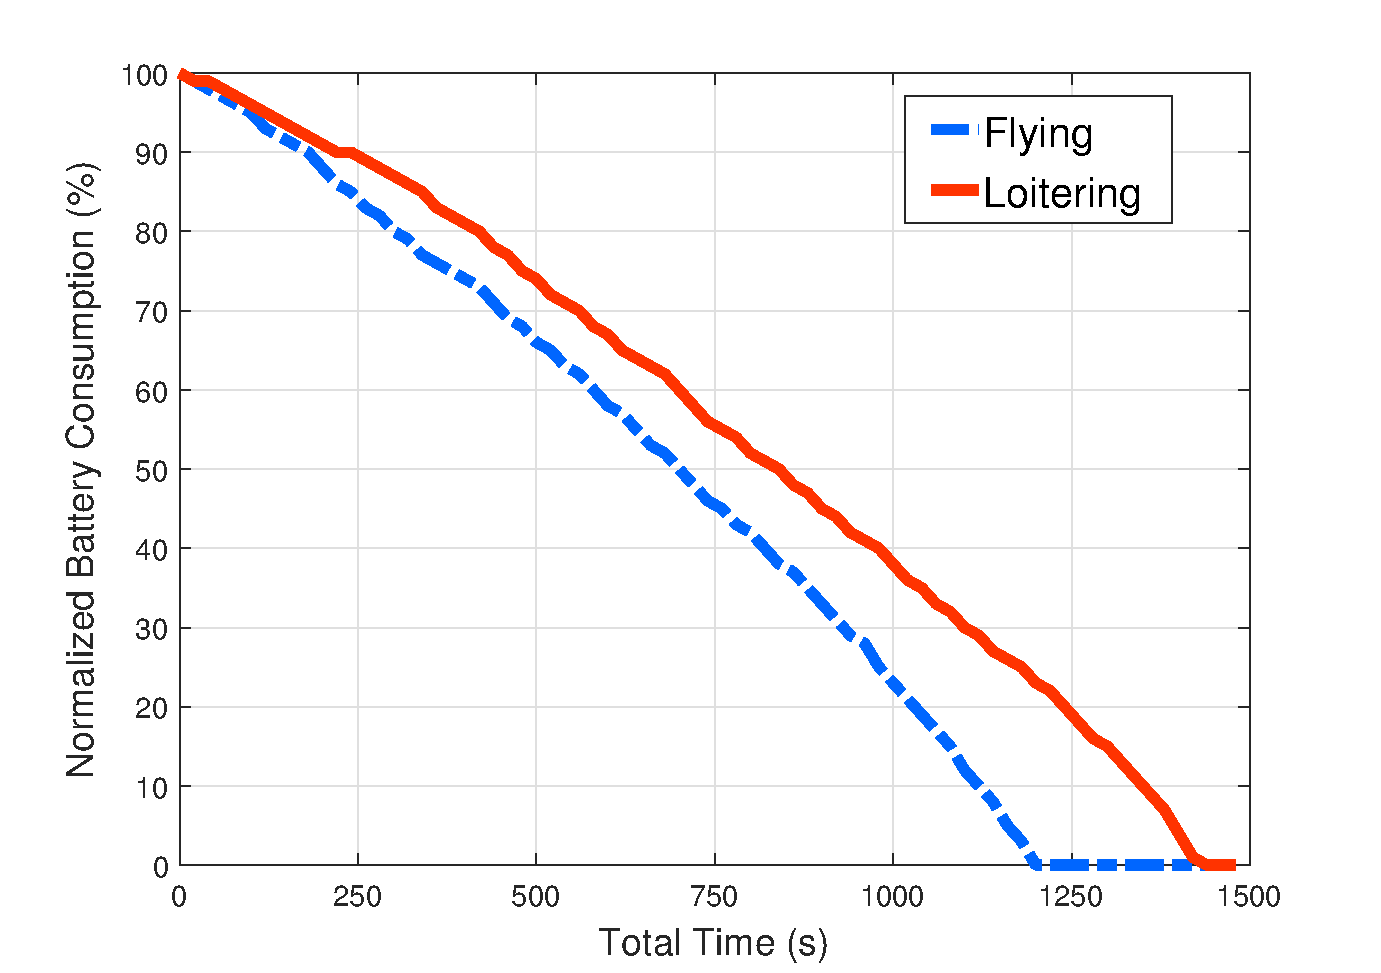
\includegraphics[width=0.5\linewidth]{pix/sensing-traj/eva_time_battery.pdf}
\caption{The flight mode consumes more battery power than the hovering mode when flying a DJI Phantom 3 quadcopter. }
\label{fig:eva_time_battery}
\end{figure}

% ÕâƪÎÄÕµĹ±Ï×£¿
% problem formulation ¡ª¡ª spanning tree/route problem?
% ×îÓÅËã·š
% ¶àžö³¡Ÿ°ÏµÄʵÑéÑéÖ€¡¢·ÂÕæ¡£
In this paper, we study the optimal trajectory planning problem of a drone for 3D space mobile sensing applications. We extend the concept of dominating set in graph theory, define a new concept called the dominating path, %xxx
and formulate the problem as finding the minimum dominating path in the grid to cover the sensing scope in 3D space with the minimum trajectory. By dividing the 3D space into a grid of observation locations (OLs), we propose a strategy that first determines the minimum dominating path of the drone that maximizes the sensing scope, and then selects an appropriate number of critical OLs within the path to perform measurement.

% get size of COL and OL-path in O(1)
According to the proposed strategy, we are able to calculate the length of the trajectory and the number of critical OLs by $O(1)$ time; and to draw the trajectory and select critical OLs in $O(\mathbb{N})$ time where $\mathbb{N}$ is the total number OLs in the grid. Our experimental results reveal that the proposed algorithm outperforms existing algorithms in two aspects: (1) the proposed solution takes 32\% less time than other solutions to complete sensing the same space; (2) during the battery life, the proposed one can reach 19\% more sensing scope than existing approaches.

%Specifically, we consider the following two special cases:
%\begin{enumerate}
%\item \emph{Consider flight time only}: Under this condition, we assume measurement time negligible and consider flight time only. We choose the shortest OL-path in OL-network to minimize flight time and select all OLs in OL-path as COLs. Therefore, we could formulate problem as a minimum dominating path. In this paper, we solved this problem in grid which could extend to three-dimensional space.
%\item \emph{Consider total time consuming}: Under this condition, we consider total time consuming which is the sum of flight time and measurement time. Since flight time usually take up most of time consuming, we find the shortest OL-path first. Then in order to minimize measurement time, we select least OLs in OL-path to cover OL-network. Also, we solve this problem in grid.
%\end{enumerate}



\section{Related Work}~\label{sec:related}

\subsection{Drones in 3D mobile sensing}
Conventional mobile sensing systems rely on the mobile devices or ground-vehicles to perform the environmental sensing in a 2D plane, e.g., the mobile data analysis using robots~\cite{brooks1986robust}, bikes~\cite{eisenman2009bikenet} or cars~\cite{devarakonda2013real}.

%BikeNet: A mobile sensing system for cyclist experience mapping :
%BikeNet represents the first comprehensive mobile sensing system quantifying the cyclist experience and provides for the collection and analysis of personal performance and communal environmental sampling. BikeNet supports two modes of operation in support of delay-tolerant and real-time sensing, and collected data can be presented both locally to the cyclist or to others via back end services.
%
%Real-time Air Quality Monitoring Through Mobile Sensing in Metropolitan Areas:
%The first work that study the long-term stability, reliability and impact of realtime pollution monitoring systems using commodity sensors and the problems associated in deploying such systems.  Present a vehicular-based mobile approach for measuring fine-grained air quality in real-time.



Drones become more and more popular in 3D mobile sensing applications since they could capture different dimensions of signals in the 3D environment that are usually beyond our sensing capability.
Aerial photo or video-graphy applications~\cite{Newman2014Drone} facilitate the collection of images, and the analysis over the collected data. For example, it is feasible to locate anomalies in image data, and link particular image data to an address of the property where the anomaly is detected. DroneSense is a system for 3D wireless signal survey~\cite{Yu2016Automating}, i.e., measuring wireless signals in the 3D space, which provides us with an efficient method to quickly analyze wireless coverage and test their wireless propagation models. SensorFly is designed for indoor emergency response or inspections in inaccessible places where people cannot reach~\cite{Purohit2011SensorFly}, which forms aerial sensor network platform that can adapt to node and network disruptions in harsh environments.


However, these 3D mobile sensing applications of drones are constrained by the limited battery life, which motivates a more efficient measurement approach to better design the trajectory.



\subsection{Trajectory planning problem}
To address the trajectory planning problem, the genetic algorithm~\cite{Hu2006A,Yun2011Improved} and particle swarm optimization~\cite{Fu2012Phase} are always proposed for real-time path planning, which could find an optimal or near-optimal path for robotics in both complicated static and dynamic environments. These approaches have been applied on the UAV platform which could ensure partial minimality between two nodes.

Meanwhile, the trajectory planning for a large scale mobile sensing scenario is usually formulated as an ordinary Travelling Salesman Problem (TSP) or a special TSP problem~\cite{Tekdas2009Using,Savla2005On}.
Existing solutions take a two-step approach: (1) the first step is to find a minimum vertex cover in the underlying network graph (i.e., a number of measurement locations that cover the given sensing area); and (2) the second step is to find the shortest path connecting these vertices (locations), along which the mobile device can traverse to complete the mobile sensing task in space.

% Some heuristic algorithms, like Life~Long~A*~\cite{Koenig2004Lifelong}, are developed to repeatedly searches for the shortest path from a given source vertex to a given destination vertex in the network graph where the cost over edges can be changing over time.

In this paper, we take a different approach by finding the optimal path first and then selecting the measurement locations, as the flight consumes more battery than hovering for drone operations.

% give a different approach that reverses order of path finding and locations selecting, and we will give an algorithm based on graph theory which could be optimal if considering flight time only.


\section{System Model and Problem Formulation}~\label{sec:problem}
% Ä£·Â mobicom£¬Õâžösection ŸÍÊÇ°Ñ Äã׌±ž¹€×÷£¬¶šÒå¡¢ž÷ÖÖÆ̵涌ЎºÃ£¬È»ºóÏÂÒ»žö section ŸÍ¿ÉÒÔÐŽœâ·šºÍÖ€Ã÷ÁË
% ÀýÈ磬3d ¿ÕŒäÔõÃŽ·Ö£¬ÔõÃŽ¶šÒåһЩ±äÁ¿
% È»ºó£¬problem formulation£¬µÃµœÒ»žöproblem£¬ŸÍÊÇÎÒÃÇÐèÒªÇóœâµÄÄ¿±ê
In this section, we establish a multi-layer 3D network model that are formed by multiple 2D networks for mobile sensing in the 3D space. Then, we formulate the problem as a combination of the minimum dominating path problem and the constrained minimum dominating set problem.

% We will make further discussion in next subsection. Finally, we define variables that would be used to mathematical proof next section.

% ÐγÉ3D OLÍøÂ磬²¢ÇÒ¶šÒåOLµÄLevel
\subsection{3D network model}
\begin{figure}[!t]
\small
\centering
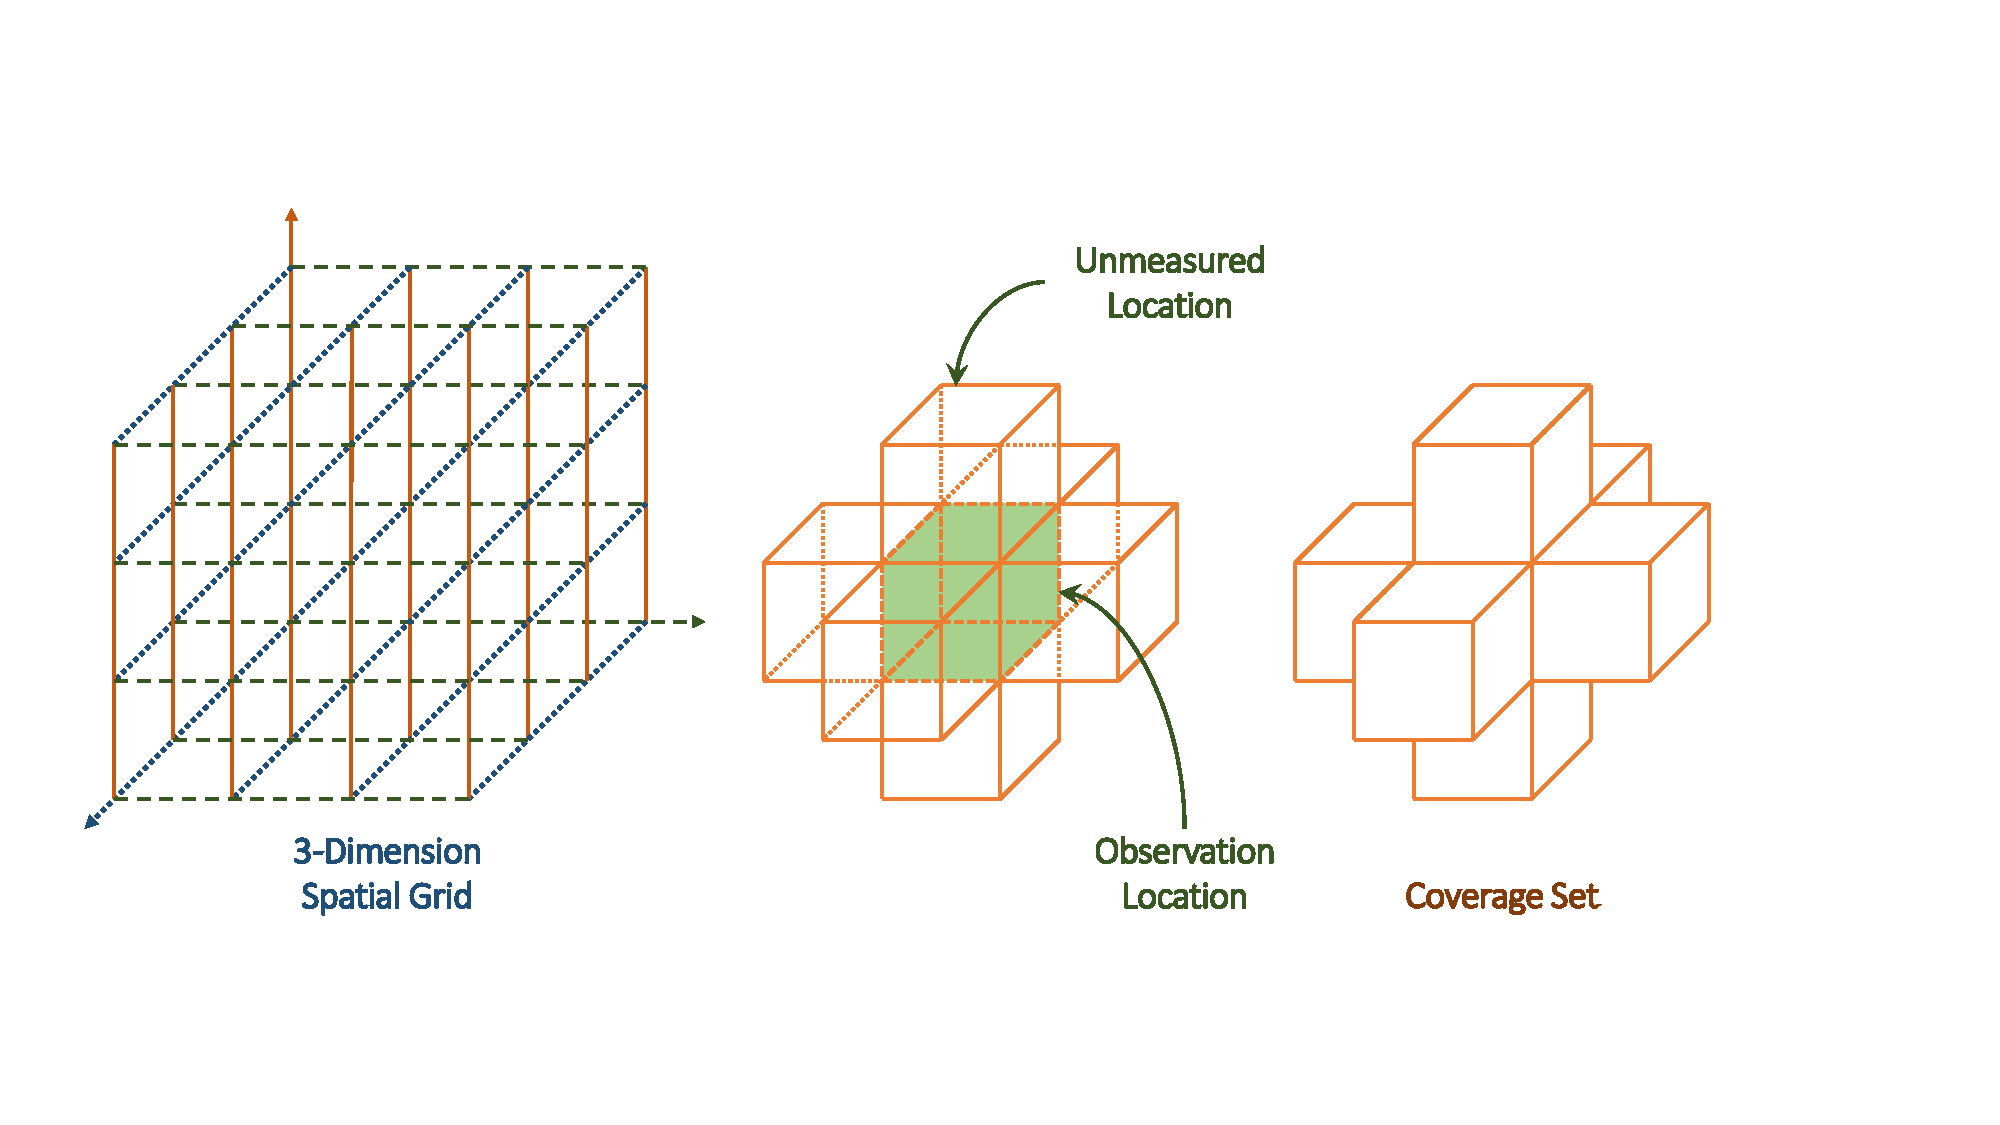
\includegraphics[width=3.3in]{pix/sensing-traj/cuboids.pdf}
\caption{The divided cuboids of a 3D space; a center OL in the cuboid in the green color; and the OLs and their cuboids in the coverage set of the center OL.}
\label{fig:cuboid}
\end{figure}

%XXX a figure
\textbf{Dividing the 3D space into cuboids}: We divide a 3D space into cuboids with $a$ meters long, $b$ meters wide and $h$ meters high. We define the center point of cuboid $i$ as its observation location (OL) (as shown in Figure~\ref{fig:cuboid}), which is denoted by the 3-tuple (longitude, latitude, and altitude), i.e.,
\[
OL_i=(x_i, y_i, z_i),
\]
where $x_i, y_i, z_i$ are 3D coordinates of OL~$i$. Note that we call the OL at the center of cuboid $i$ as OL~$i$.

\textbf{3D network of observation locations (OLs)}: OLs form a 3D network graph $\mathcal{G}=(\mathcal{V};\mathcal{E})$, where $\mathcal{V}$ denotes the set of vertices and $\mathcal{E}$ represents the edges connecting neighboring vertices. Specifically, the OL inside each cuboid~$i$ is considered as a vertex in $\mathcal{G}$, and an edge $(i,j)$ exists, if cuboid~$i$ is adjacent to cuboid $j$ (i.e., they are the same in two coordinates and adjacent to each other in the third dimension coordinate). As a result, %xxx
the OLs forms a 3D grid in the space.

\textbf{The coverage set of OL~$i$}: We define the coverage set of OL~$i$ as the set of OLs including those located in the neighbor cuboids of the cuboid~$i$, plus OL~$i$ itself, as shown in Figure~\ref{fig:cuboid}.


\textbf{Critical OL (COL)}: Given limited battery life, it is impossible for a drone to traverse all OLs in the space. Hence, we need to select a number of critical observation locations (COL) from OLs where the drone can perform the measurement.


\textbf{Correlation between OLs}: We assume that the sensed data at two OLs in the same 3D space may have certain correlation. Intuitively, the more distant two OLs are located, the less correlation they may have. That is, two adjacent OLs have the strongest correlation in their sensed data; the sensed data at two adjacent OLs are almost the same if the distance between them is small. Hence, if the drone has sensed at one OL, it can skip sensing at its adjacent OLs.

\textbf{Multiple layers of 2D grids}: The 3D grid can be divided into multiple layers of 2D grids at different heights. If the drone has sensed at OLs in one layer of 2D grid, it can skip sensing at OLs in its adjacent layers of 2D grids (i.e, the one upper layer and the one lower layer). Let $G=L_{m,n}=(V;E)$ denote a 2D grid with $m$ rows and $n$ columns.


\subsection{Time consumed}
The time consumed by the 3D mobile sensing of drones consists of two parts: (1) the flight time, and (2) the measurement time.

Let $V_C \subseteq V$ denote the set of COLs, and $v_{C_i}$ is the $i$-th vertex in $V_C$. Let $V_P \subseteq V$ denote the set of vertices in the drone's trajectory which forms a path in $\mathcal{G}$. We have $V_C \subseteq V_P$ since the trajectory should contain the COLs, i.e., vertices in $V_C$.


\textbf{Flight time}: the flight time $T_F$ is time consumed by the drone's flight. In the formed 3D grid, we use Hamiltonian distance to characterize the distance between OLs. So the flight time is proportion to the length of the trajectory, which is written as
$
T_F=t_F |V_P|,
$
where $t_F$ is the flight time for a unit length in the coordinate system of the 3D grid.

\textbf{Measurement time}: the measurement time $T_M$ is time consumed by the drone for hovering and measurement. For the same sensing task (e.g., WiFi signal survey), we could assume that measurement time is the same for all OLs. So the total measurement time is proportion to the number of COLs, which can be written as
$
T_M=t_M |V_C|,
$
where $t_M$ is the measurement time at each OL.

Therefore, the total time $T$ consumed by the drone is
\[
T=T_F + T_M.
\]

\subsection{Problem formulation}
% Given a 3D space, we first establish a 3D OL network $G=(V;E)$ which forms a 3D grid. Each OL in grid has a coverage set. Due to drones' limited battery life, we want to complete flight in the shortest time. Hence, in order to minimize total time consuming, we select COLs from OLs to cover OL-network while find a OL-path(trajectory) covers COLs. We formulate this problem as a constraint set coverage problem in 3D grid.

%We formulate the following two problems based on two observations: (1) the flight mode consumes more battery per unit time than the hovering mode for a drone; (2) the flight time is much more than the measurement time in the trajectory for most sensing applications.
%
%\subsubsection{Case~1: Considering flight time only}
%In this case, we assume the flight time is dominant, and the measurement time at each OL can be negligible. Then, we formulate the problem as a minimum dominating path problem in multi-layer 2D grids.
%\begin{prob}[Trajectory planning by flight time only]\label{prob:flight-time-only}
%Given a 3D grid $\mathcal{G}$ divided into multi-layer 2D grids, for each 2D grid $G=L_{m,n}=(V;E)$ where $V=\{v_0, v_1, ..., v_{|V|-1} \}$, assume the time required for completing a drone's trajectory is only relevant to the drone's flight time, and let %xxx variable same
%$C(v_i)$ be the coverage set of vertex $v_i$ in $V$.
%
%
%Since $V_C=V_P$, we seek to find the minimum dominating path $V_P \subseteq V$ which contains COLs in $V$ and covers all OLs in the 3D grid.
%\[
%\begin{aligned}
%& \text{minimize}
%& & \;|V_P| \\
%& \text{subject to}
%& & \bigcup_{v \in V_P} C(v)=V, ~~\;V_P \; is \;a \; path.
%\end{aligned}
%\]
%\end{prob}
%
%
%\subsubsection{Case~2: Considering both flight time and measurement time}
%%xxx no col select
%In this case, we assume the measurement time at each OL is not negligible. As the flight mode consumes more power per unit time, we first search for the shortest path that has the maximum coverage, and then select the least number of OLs along the path as COLs for measurement.

We formulate this problem as a combination of a minimum dominating path problem and a constrained minimum dominating set problem in multi-layer 2D grids.

\begin{prob}[Trajectory planning by both flight time and measurement time]

Given a 3D grid $\mathcal{G}$ divided into multi-layer 2D grids, for each grid $G=L_{m,n}=(V;E)$ where $V=\{v_0, v_1, ..., v_{|V|-1} \}$, assume the time required for completing a drone's trajectory is dependent on the drone's flight time and measurement time, and let $Cov(v_i)$ be the coverage set of vertex $v_i$ in $V$.


We seek to find the minimum dominating path $V_P \subseteq V$ which covers all OLs in the 3D grid, and then select a set $V_C$ of COLs from $V_P$ as the dominating set.
\[
\begin{aligned}
& \text{minimize}
& & \;|V_P|,\;|V_C| \\
& \text{subject to}
& & \bigcup_{v \in V_P} Cov(v)=V,~~ \bigcup_{v \in V_C} Cov(v)=V,\\
&&& \;V_P \; is \;a \; path, ~~ \;V_C \subseteq V_P.
\end{aligned}
\]
\end{prob}

Therefore, we will discuss this problem in the next section and give corresponding certification.


\section{Optimal Trajectory Planning Mechanism}
In this section, we first extend the well-known concept of the dominating set to define the dominating path in a graph.
Then, we address Problem~1 by proposing an optimal algorithm to find the minimum dominating path and the dominating set in the path in the 2D grid. We can concatenate the discovered paths (trajectories) in 2D grids to construct one in the 3D grid.

\subsection{From the dominating set to dominating path}
\begin{figure}[htbp]
\begin{subfigure}[t]{0.3\linewidth}
\centering

\includegraphics[width=0.7\linewidth]{pix/sensing-traj/dominating_set.pdf}
\caption{}
\vspace{0.12in}
\label{fig:dominating_set}
\end{subfigure}%
\hfill
\begin{subfigure}[t]{0.3\linewidth}
\centering

\includegraphics[width=0.7\linewidth]{pix/sensing-traj/con_dominating_set.pdf}
\caption{}
\label{fig:con_dominating_set}
\end{subfigure}
\hfill
\begin{subfigure}[t]{0.3\linewidth}
\centering

\includegraphics[width=0.7\linewidth]{pix/sensing-traj/dominating_path.pdf}
\caption{}
\label{fig:dominating_path}
\end{subfigure}
\caption{A (a) dominating set, (b) connected dominating set, (c) dominating path of $L_{8,7}$. In dominating path, orange vertices are dominating vertices and green vertices are connecting vertices.}
\label{fig:dominating_path_difference}
\end{figure}

% XXX add a figure to explain how to extend dominating path, and what are dominating path vertices

\textbf{Our definition of dominating path}: Recall that a dominating set for the graph $G=(V,E)$ is a subset $D \subset V$ such that every vertex not in $D$ has a neighbor on $D$. A connected dominating set $D$ for graph $G=(V,E)$ is a special dominating set such that any vertex in $D$ can reach any other node in $D$ by a path that stays entirely within $D$.
Similarly, we have the following definition.
\begin{defn}~\label{lem:3extend}
A dominating path for graph $G=(V,E)$ is a path $P \subset V$ such that every vertex not in $P$ has a neighbor on $P$ which is a special connected dominating set. In a dominating path $P$,
\begin{itemize}
  \item there exists a dominating set $D_P$ of $G$, and vertices in $D_P$ are called \emph{dominating vertices} of path $P$;
  \item and the other vertices in $P \setminus D_P$ are called \emph{connecting vertices} of path $P$.
\end{itemize}
\end{defn}
We show difference among dominating set, connected dominating set and dominating path in Figure~\ref{fig:dominating_path_difference}.

\begin{figure}[htbp]
\begin{subfigure}[t]{0.23\linewidth}
\centering

\includegraphics[width=0.4\linewidth]{pix/sensing-traj/trivial_step_1.pdf}
\caption{A minimum dominating path of $L_{3,3}$;}
\vspace{0.12in}
\label{fig:trivial_step_1}
\end{subfigure}%
\hfill
\begin{subfigure}[t]{0.23\linewidth}
\centering

\includegraphics[width=0.8\linewidth]{pix/sensing-traj/trivial_step_2.pdf}
\caption{A minimum dominating path of $L_{3,6}$;}
\label{fig:trivial_step_2}
\end{subfigure}
\hfill
\begin{subfigure}[t]{0.23\linewidth}
\centering

\includegraphics[width=0.4\linewidth]{pix/sensing-traj/trivial_step_3.pdf}
\caption{A minimum dominating path of $L_{6,3}$;}
\label{fig:trivial_step_3}
\end{subfigure}
\begin{subfigure}[t]{0.23\linewidth}
\centering

\includegraphics[width=0.8\linewidth]{pix/sensing-traj/trivial_step_further.pdf}
\caption{A minimum dominating path of $L_{6,6}$;}
\label{fig:trivial_step_further}
\end{subfigure}
\caption{A complete process from minimum dominating path in $L_{3,3}$ to minimum dominating path in $L_{6,6}$.}
\label{fig:trivial_steps}
\end{figure}

\textbf{Start from the trivial cases}: The goal is to find the minimum dominating path in a 2D grid $L_{m,n}$, where $m,n$ are positive integers.
\begin{itemize}
  \item \emph{Step~1: trivial cases}. When $m\leq 3$ and $n\leq 3$, it is easy to find the minimum dominating path;
  \item \emph{Step~2: adding more columns to trivial cases}. When $m\leq 3$ and $ 3< n \leq 6$, we seek to construct the minimum dominating path in the 2D grid  $L_{m,n}$ by extending the minimum dominating path in the 2D grid  $L_{m,(n-3)}$ that has been found in Step~1;
  \item \emph{Step~3: adding more rows to trivial cases and transposing the grid}. When $3< m \leq 6$ and $ n\leq 3$, we first transpose the grid---swap the rows and columns of the grid, and construct the minimum dominating path in the 2D grid $L_{n,m}$ by following Step~2;
\end{itemize}
Any bigger-size grid $L_{m,n}$ when $3< m \leq 6$ and $3< n \leq 6$ can be expended by adding three more rows and/or three more columns from one of the grids in trivial cases. The minimum dominating path in the bigger-size grid $L_{m,n}$ can be also found by repeating above Steps~2 and~3. A complete process from minimum dominating path in $L_{3,3}$ to minimum dominating path in $L_{6,6}$ is shown in Figure~\ref{fig:trivial_steps}.

Next, we show the correlation between the smaller grid $L_{m,n}$ and the expanded grid $L_{m,(n+3)}$; note that the latter is expanded by adding three columns to the former.

%We give notations of variables.
%\begin{itemize}
% \item $c_i$: Leftmost $i-th$ column in grid $G$.
%  \item $r_i$: Topmost $i-th$ row in grid $G$.
%  \item $C_{i,j}$: Columns between $c_i$ and $c_j$.
%  \item $R_{i,j}$: Rows between $r_i$ and $r_j$.
%  \item $v_{i,j} = r_i \cap c_j$: Vertex of intersection of $i$-th row and $j$-th column in grid.
%  \item $N[y]$: Coverage set of vertex $y$.
%  \item $N[S]$: Coverage set of vertices in set $S \subset V$.
%  \item $P^c_i=P \cap c_i$: Intersection between $P$ and column~$c_i$.
%  \item $P^r_i=P \cap r_i$: Intersection between $P$ and row-$r_i$.
%  \item $P^c_{i,j}=P \cap C_{i,j}$: Intersection between $P$ and columns~$C_{i,j}$.
%  \item $P^r_{i,j}=P \cap R_{i,j}$: Intersection between $P$ and rows~$R_{i,j}$.
  %XXXXXXXXXXXXXXXX
%  \item $D(P)$: Dominating vertices in path~$P$.
%  \item $C(P)$: Connecting vertices in path~$L$.
  %\item $D^c_i(P)$: Dominating vertex in $P^c_i$.
%  \item $D^r_i(P)$: Dominating vertex in $P^r_i$.
%  \item $D^c_{i,j}(P)$: Dominating vertices in $P^c_{i,j}$.
%  \item $D^r_{i,j}(P)$: Dominating vertices in $P^r_{i,j}$.
%  \item $C^c_{i,j}(P)$: Connecting vertices that connect vertices in $D^c_{i,j}(P)$.
%  \item $C^r_{i,j}(P)$: Connecting vertices that connect vertices in $D^r_{i,j}(P)$.
%  \item $C^{con}_{i}(P)$: Connecting vertices that connect vertices between $D^c_{1,i}(P)$ and $D^c_{i+1,n}(P)$.
%  \item $\gamma(G)$: The size of minimum dominating set of $G$.
%  \item $\gamma_c(G)$: The size of minimum connected dominating set of $G$.
%  \item $\gamma_p(G)$: The size of minimum dominating path of $G$.
%  \item $G^c_i$: Leftmost $i-th$ column in grid $G$.
%  \item $G^r_i$: Topmost $i-th$ row in grid $G$.
%  \item $G^c_{i,j}$: Columns between $G^c_i$ and $G^c_j$.
%  \item $G^r_{i,j}$: Rows between $G^r_i$ and $G^r_j$.
%  \item $v_{i,j}$: Vertex of intersection of $G^r_i$ and $G^c_j$ in grid.
%  \item $N[y]=\{v,y\in V: yv\in E\} \cup \{y\}$: Coverage set of vertex $y$.
%  \item $N[S]= \bigcup_{v \in S} N[v]$: Coverage set of vertex set $S \subset V$.
%  \item $L^c_i=L \cap G^c_i$: Intersection between $P$ and $G^c_i$.
%  \item $L^r_i=L \cap G^r_i$: Intersection between $P$ and $G^r_i$.
%  \item $L^c_{i,j}(G)=L \cap G^c_{i,j}$: Intersection between $L$ and $G^c_{i,j}$.
%  \item $L^r_{i,j}(G)=L \cap G^r_{i,j}$: Intersection between $L$ and $G^r_{i,j}$.
%  \item $D(L)$: Dominating vertices in $L$.
%  \item $C(L)$: Connecting vertices in $L$.
%  \item $D^c_i(L)$: Dominating vertex in $L^c_i$.
%  \item $D^r_i(L)$: Dominating vertex in $L^r_i$.
%  \item $D^c_{i,j}(L)$: Dominating vertices in $L^c_{i,j}(G)$.
%  \item $D^r_{i,j}(L)$: Dominating vertices in $L^r_{i,j}(G)$.
%  \item $C^c_{i,j}(L)$: Connecting vertices that connect vertices in $D^c_{i,j}(L)$.
%  \item $C^r_{i,j}(L)$: Connecting vertices that connect vertices in $D^r_{i,j}(G)$.
%  \item $C^{ccon}_{i}(L)$: Connecting vertices that connect vertices between $D^c_{1,i}(L)$ and $D^c_{i+1,n}(L)$.
%  \item $\gamma(G)$: The size of minimum dominating set of $G$.
%  \item $\gamma_c(G)$: The size of minimum connected dominating set of $G$.
%  \item $\gamma_l(G)$: The size of minimum dominating path of $G$.
%\end{itemize}


% Ö€Ã÷ÏÖÓÐœá¹û
\subsection{The size of the minimum dominating path in the expanded grid $L_{m,{n+3}}$}

\subsubsection{How many vertices are needed for constructing the minimum dominating path in $L_{m,n+3}$}
The grid $L_{m,n+3}$ can be divided into two parts: (1) the left part grid from the 1st to the $n$-th columns, and (2) the right part from the $(n+1)$-th to the $(n+3)$-th columns. The left part is basically a smaller grid of $L_{m,n}$.

%xxx
Given the grid $L_{m,{n+3}}$, we will derive the minimum number of vertices needed to add into the minimum dominating path of left part grid (i.e., $L_{m,n}$), so as to construct the minimum dominating path in $L_{m,{n+3}}$.

Since vertices in a dominating path $P$ consists of dominating vertices ($D(P)$) and connecting vertices ($C(P)$), we could split $P$ of $L_{m,n+3}$ into 5 parts: dominating vertices from the 1st to the $n$-th columns ($D^c_{1,n}(P)$), dominating vertices from the $(n+1)$-th to the $(n+3)$-th columns ($D^c_{n+1,n+3}(P)$), connecting vertices that connect vertices in $D^c_{1,n}(P)$ ($C^c_{1,n}(P)$), connecting vertices that connect vertices in $D^c_{n+1,n+3}(P)$ ($C^c_{n+1,n+3}(P)$) and connecting vertices that connect vertices between $D^c_{1,n}(P)$ and $D^c_{n+1,n+3}(P)$ ($C^{con}_{n}(P)$).

To simplify proof, we also give some notations of variables. $c_i$ denotes leftmost $i$-th column of $L_{m,n+3}$. $r_i$ denotes topmost $i$-th row of $L_{m,n+3}$. $C_{i,j}$ denotes columns between $c_i$ and $c_j$. $v_{i,j} = r_i \cap c_j$ denotes the intersection of $i$-th row and $j$-th column in $L_{m,n+3}$. $P^c_i=P \cap c_i$ denotes intersection between $P$ and column~$c_i$. $P^c_{i,j}=P \cap C_{i,j}$ denotes intersection between $P$ and columns~$C_{i,j}$. $D^c_i(P)$ denotes dominating vertices in $P^c_i$. $N[y]$ denotes coverage set of vertex $y$ and $N[S]$ denotes coverage set of vertices in set $S \subset V$. $\gamma_p(G)$ denotes the size of the minimum dominating path of graph $G$.

% Since vertices in $L$ consists of dominating vertices and connecting vertices, we split dominating path in $L_{m,n+3}$ into 5 parts: $L=D^c_{1,n}(L) \cup D^c_{n+1,n+3}(L) \cup C^c_{1,n}(L) \cup C^c_{n+1,n+3}(L) \cup C^{ccon}_{n}(L)$.


\begin{figure}[htbp]
\begin{subfigure}[t]{0.45\linewidth}
\centering

\includegraphics[width=0.7\linewidth]{pix/sensing-traj/lem2_prob.pdf}
\caption{}
\vspace{0.12in}
\label{fig:lem2_prob}
\end{subfigure}%
\hfill
\begin{subfigure}[t]{0.45\linewidth}
\centering

\includegraphics[width=0.66\linewidth]{pix/sensing-traj/lem2_sol.pdf}
\caption{}
\label{fig:lem2_sol}
\end{subfigure}
\hfill
\caption{(a) 3 continuous vertices in $c_n$ dominated by $D^c_{n+1}(P)$. Circle vertices are vertices in $P$, star vertices are vertices in $v_{k'}$, triangle vertices are vertices in $v_k$; (b) Part of $P'$ that could replace $P$.}
\label{fig:lem2}
\end{figure}

\begin{lem}~\label{lem:ndominating}
Let $P^*$ denote a minimum dominating path of $L_{m,n}$. Then there exists at least one minimum dominating path $P$ in $L_{m,(n+3)}$, such that the number of dominating vertices of path $P$ from the 1st to the $n$-th columns is no less than the number of dominating vertices of path $P^*$. That is, $|D^c_{1,n}(P)| \geq |D(P^*)|$.
% In other words, none of vertices in $G^c_{1,n}$ is covered by $D^c_{n+1,n+3}(L)$.
\end{lem}

\begin{proof}
We have $|D^c_{1,n}(P)| \geq |D(P^*)|$ if all vertices in $C_{1,n}$ is dominated by $D^c_{1,n}(P)$ since $C_{1,n}=L_{m,n}$. Therefore, if $|D^c_{1,n}(P)|<|D(P^*)|$, some vertices in $c_n$ must be dominated by $D^c_{n+1}(P)$ and do not have neighbors in $D^c_{1,n}(P)$.

Consider there are $k$ continuous vertices $v_k$ in $c_n$ dominated by $D^c_{n+1}(P)$.

If $k \geq 2$, since these $k$ vertices are not dominated by $D^c_{1,n}(P)$, the corresponding $k$ vertices $v_{k'}$ which are in the same row with $v_k$ in $c_{n-1}$ can not belong to $D^c_{1,n}(P)$. Therefore, k vertices $v_{k''}$ in $c_{n-2}$ should belong to $D^c_{1,n}(P)$ to dominate $v_{k'}$ because only two end points in $v_{k'}$ could be dominated by its top and bottom vertices instead, but their right neighbors could not belong to $P$ which makes $P$ irregular. Therefore, we have $v_{k''} \subset P$ and we could use $v_{k''}$ to construct, as shown in Figure~\ref{fig:lem2_prob}.

Since $C_{n+1,n+3}$ may have multiple connected components, $P$ may step into $C_{n+1,n+3}$ and finish trajectory or move out from $C_{n+1,n+3}$.

In the first case, we could construct a dominating path $P'$ as Figure~\ref{fig:lem2_sol} such that $|P'|=|P|$ and none of vertices in $c_n$ is dominated by $D^c_{n+1}(P')$.

In the second case, when $D^c_{n+1}(P)$ comes from $D^c_{n+2}(P)$, we have the following three cases. When $|v_k|>3$, $P$ would need more vertices in $c_{n+3}$ to dominate vertices in $c_{n+2}$. When $|v_k|<3$, $P$ will need more connecting vertices. For these two cases, we use the same structure in Figure~\ref{fig:lem2_sol} to construct $P'$ to replace $P$. When $|v_k|=3$, assume $P$ move back to $C_{1,n}$ from row $r$. If $v_{r,n+3} \notin P$, we could use the same structure in Figure~\ref{fig:lem2_sol}. Otherwise, we consider the path extend from $r$ and vertices form a dominating path for $L_{6,k}$ partially but is not the minimum one. Therefore, $P$ could not be the minimum dominating path when $|v_k|=3$.

If $k=1$, then the vertex must lay in boundary otherwise it will need extra connecting vertices between $r_{n+1}$ and $r_{n+2}$. Therefore, we assume $v_{1,n+1} \in P$. Then $v_{1,n}, v_{1,n-1} \notin P$ and one of $v_{1,n-2}$ and $v_{2,n-1}$ must belong to $P$ to dominate $v_{1,n-1}$. If $v_{1,n-2} \in P$, $P$ will turn to $r_{n-1}$ to dominate vertices in $r_n$ and it will bring more vertices than the following condition. If $v_{2,n-1} \in P$, we have structure shown in Figure~\ref{fig:meta_struct1_b}. This case could only exist once. We could transform $L_{m,n+3}$ symmetrical. Then, we have $|D^c_{1,n}(P)| \geq |D(P^*)|$.

\end{proof}

%Given $P$ as the minimum dominating path of the grid $L_{m,n+3}$, let $D^c_{n+1,n+3}(P)$ denote the set of dominating vertices of path $P$ from the $n+1$-th column to the $n+3$-th column of grid $L_{m,n+3}$; and let $C^{con}_n(L)$ denote the set of connecting vertices of path $P$ between $D^c_{1,i}(P)$ and $D^c_{i+1,n}(P)$. Then, we have the following lemma.

Given $P$ as the minimum dominating path of the grid $L_{m,n+3}$, we have the following lemma.

\begin{lem}~\label{lem:3dominating}
The number of dominating vertices of path $P$ from the $n+1$-th to the $n+3$-th columns of grid $L_{m,n+3}$, plus the number of connecting vertices of path $P$ between the dominating vertices from the 1st to the $n$-th columns and the dominating vertices from the $n+1$-th to the $n+3$-th columns is no less than $m$. That is $|D^c_{n+1,n+3}(P)| + |C^{con}_n(P)| \geq m$. Further, if $3 \nmid m$, then $|D^c_{n+1,n+3}(P)| + |C^{con}_n(P)| \geq m+1$.
\end{lem}

% todo: $|D^c_{n+1,n+3}(P)| + |C^{con}_n(P)|$ change to origin format?
\begin{proof}
Since $c_{n+1}$ might be dominated by $D^c_{1,n}(P)$, we consider the coverage problem of $C_{n+2,n+3}$ only.

Before formal proof, we will prove that expect for one single case, $C_{n+2,n+3}$ is dominated by rows. Specifically, every row in $C_{n+2,n+3}$ is dominated by one connected component in $P^c_{n+1,n+3}$.

If $r_i$ in $C_{n+2,n+3}$ is dominated by two connected components in $P^c_{n+2,n+3}$, then we assume $v_{i,n+2}$ is dominated by a component above and $v_{i,n+3}$ is dominated by the other component beneath.

Therefore, there are two different scenarios. Under the first scenery, $r_i$ is dominated by two end vertices which can be transformed by extending one vertex to dominate all vertices dominated by two components. Under the second scenery, $r_i$ is dominated by one end point and one intermediate vertex. This is the unique case that could not be replaced. But we could merge them into one part since the union of two components follows the result.

Then, we prove the result by induction. Obviously, when $m=1$, $|D^c_{n+1,n+3}(P)| + |C^{con}_n(P)| \geq 2$, when $m=2$, $|D^c_{n+1,n+3}(P)| + |C^{con}_n(P)| \geq 3$ and when $m=3$, $|D^c_{n+1,n+3}(P)| + |C^{con}_n(P)| \geq 3$.

Now assume the result holds for $m=k$. When $m=k+1$, if there is only one connecting component in $P^c_{n+1,n+3}$, $|\gamma_p(C_{n+2,n+3})| = m$. Adding 1 connecting vertex in $c_{n+1}$, $|D^c_{n+1,n+3}(P)| + |C^{con}_n(P)| \geq m+1$. If there are multiple connecting components in $P^c_{n+1,n+3}$, we assume $C_{n+2,n+3}$ is dominated by rows. Assume $a$ rows and $b$ rows are dominated by two connected components $P_a$ and $P_b$ respectively. If $3 \mid m$, then at most two of $a$ and $b$ could be divided by 3 so that $|(D^c_{n+1,n+3}(P) \cup C^{con}_n(P)) \cap (P_a \cup P_b)| \geq a+b$. If $3 \nmid m$, then at most one of $a$ and $b$ could be divided by 3 so that $|(D^c_{n+1,n+3}(P) \cup C^{con}_n(P)) \cap (P_a \cup P_b)| \geq a+b+1$. Therefore, multiple connected components can finally reduce to one component which also holds the result.

\end{proof}


% Based on the results of Lemma~\ref{lem:ndominating} and Lemma~\ref{lem:3dominating}, we decompose a minimum dominating path in $L_{m,n+3}$ into two parts: (1) the left part from 1st column to the $n$-th column of $L_{m,n+3}$; and (2) the right part from $n+1$-th column to the $n+3$-th column of $L_{m,n+3}$.



%\begin{figure}[htbp]
%\begin{subfigure}[t]{0.45\linewidth}
%\centering
%
\includegraphics[height = 1.5 in]{pix/sensing-traj/thm4_struct_boundary.pdf}
%\caption{}
%\label{fig:thm4_struct_boundary}
%\end{subfigure}%
%\hfill
%\begin{subfigure}[t]{0.45\linewidth}
%\centering
%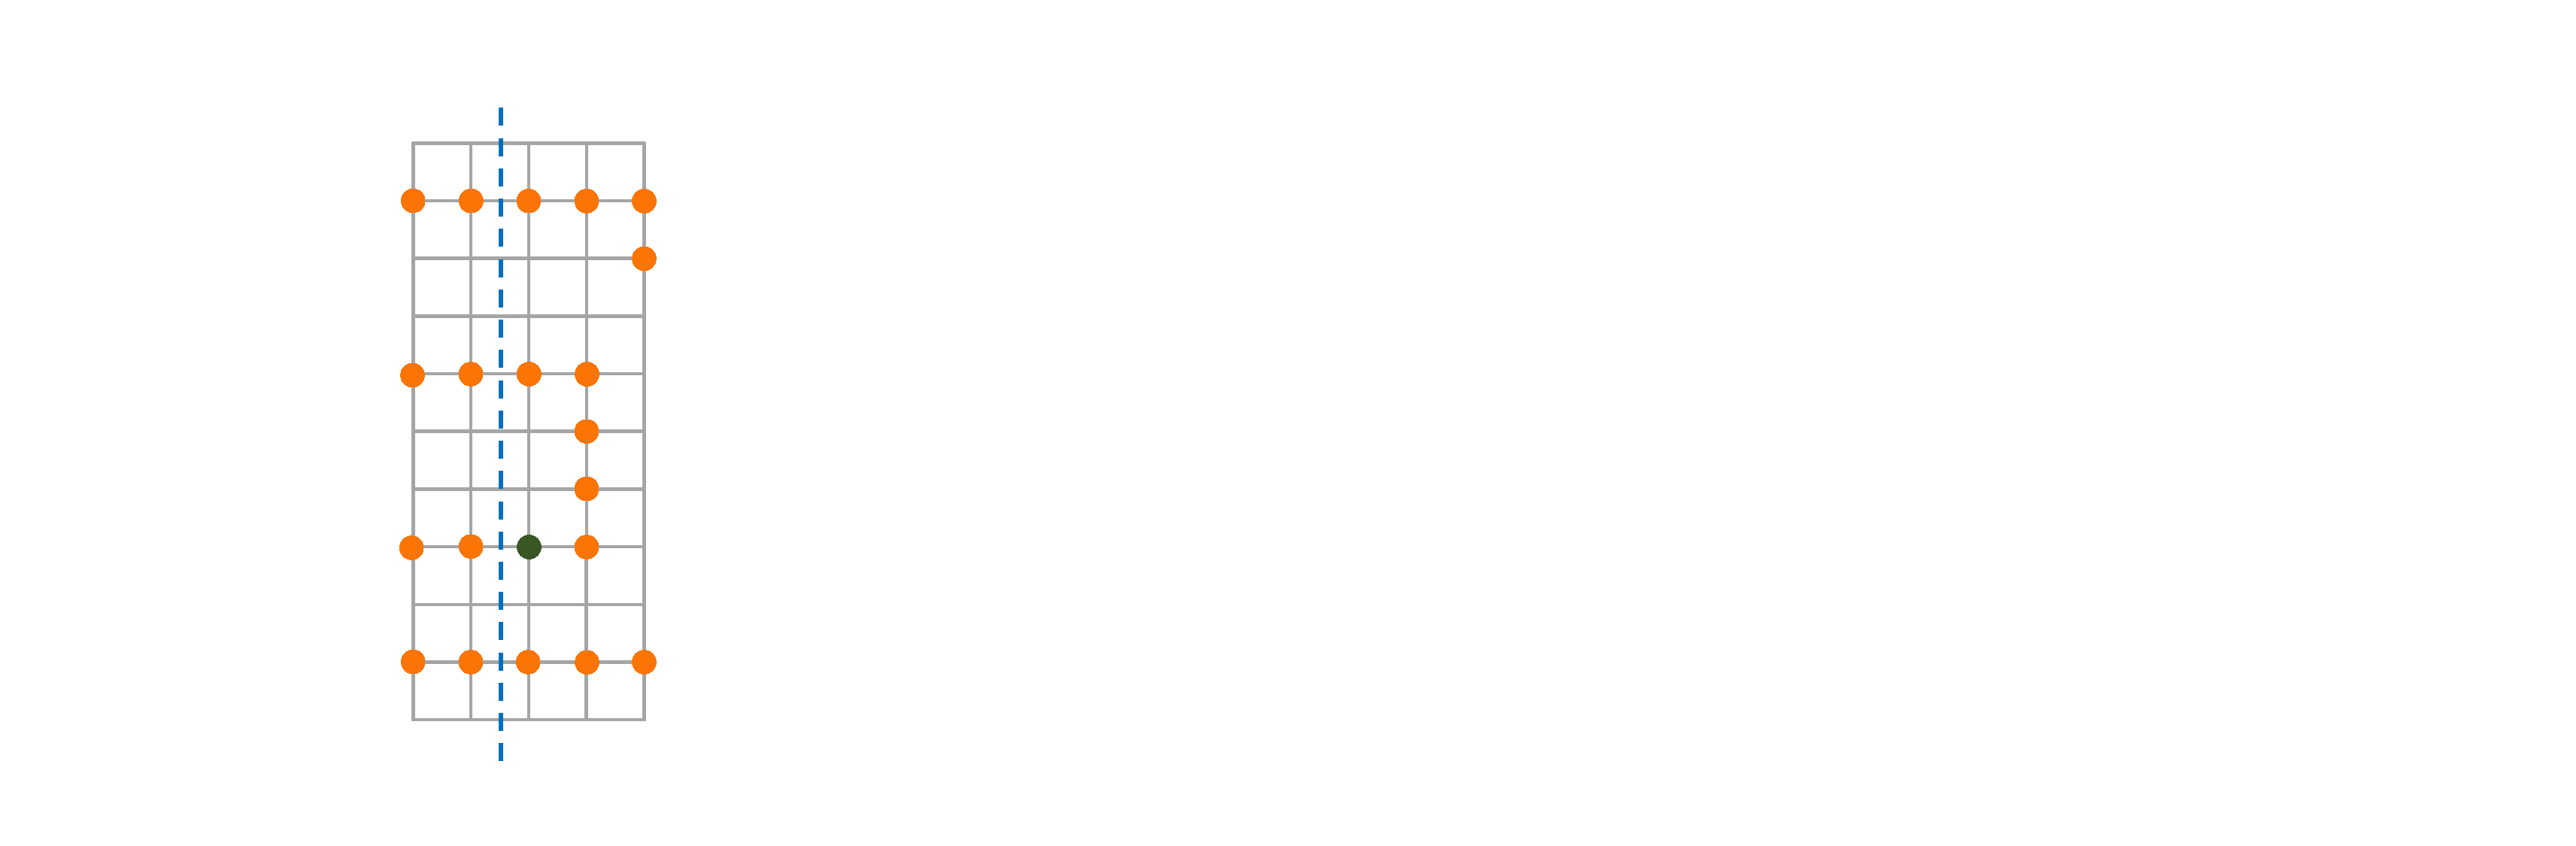
\includegraphics[height = 1.5 in]{pix/sensing-traj/thm4_period.pdf}
%\caption{}
%\label{fig:thm4_period}
%\end{subfigure}
%\hfill
%\caption{(a) Typical structure of minimum dominating path on the boundary; (b) 2-period coverage and 3-period coverage of specific structure.}
%\label{fig:lem2}
%\end{figure}

Since the left part of $L_{m,n+3}$ is a grid $L_{m,n}$, the following theorem tells the relationship between the minimum dominating paths of $L_{m,n+3}$ and $L_{m,n}$.

\begin{thm}~\label{thm:3period}
The minimum dominating path of $L_{m,n+3}$ contains at least $m$ more vertices than that of $L_{m,n}$. That is $\gamma_p(L_{m,n+3}) \geq \gamma_p(L_{m,n})+m$. Further, when $3 \nmid m$, $\gamma_p(L_{m,n+3}) \geq \gamma_p(L_{m,n})+m+1$.
\end{thm}

\begin{proof}
In Lemma~\ref{lem:ndominating} and Lemma~\ref{lem:3dominating}, we know that there exists at least one minimum dominating path $P$ in $L_{m,n+3}$ such that $|D^c_{n+1,n+3}(P)| + |C^{con}_{n}(P)| + |D^c_{1,n}(P)|$ could fulfill additive part in the result. Therefore, if the result is false, $|C^c_{1,n}(P)| + |C^c_{n+1,n+3}(P)|$ must be less than $C(P^*)$ which is the connecting vertices of a minimum dominating path $P^*$ in $L_{m,n}$.

\textbf{Connectivity on the boundary}:
Since connectivity depends on structure of $r_n$ and there are only two end vertices in $P$, we have structures in $r_n$ like Figure~\ref{fig:thm4_struct_boundary}. We will consider different structures of $P$ in $r_n$.

If there are only one connecting vertex $v_{i,n}$ in a connected component, we have following two cases. In the first case, we have $v_{i-1, n+1}$, $v_{i-1, n+2}$, $v_{i+1, n+1}$, $v_{i+1, n+2}$, $v_{i, n+2} \in P$. In this case, although $v_{i-1, n+1}, v_{i+1, n+1} \in C^{con}_n(P)$ which decreases $|C^c_{1,n}(P)| + |C^c_{n+1,n+3}(P)|$, but we still use 4 addition vertices to dominate 3 rows. In the second case, we have $v_{i-1, n+1}$, $v_{i-1, n+2}$, $v_{i-1, n+3}$, $v_{i+1, n+1}$, $v_{i+1, n+2}$, $v_{i+1, n+3}$, $v_{i, n+3} \in P$ which still hold $|C^c_{1,n}(P)| + |C^c_{n+1,n+3}(P)|=|C(P^*)|$ partially.

If there are two connecting vertices in one connected component, when we consider them separately, result is the same as one connecting vertex. If we consider them together, the size of $P$ in the component in $r_n$ must be 4. We assume the two vertices are $v_{i,n}$ and $v_{i+1,n}$. Also, we have two cases. In the first case, we have $v_{i-1, n+1}$, $v_{i-1, n+2}$, $v_{i-1,n+3}$, $v_{i,n+3}$, $v_{i+1, n+3}$, $v_{i+2, n+1}$, $v_{i+2, n+2}$, $v_{i+2, n+3} \in P$, which hold $|C^c_{1,n}(P)| + |C^c_{n+1,n+3}(P)|=|C(P^*)|$ partially. In the second case, we have $v_{i-1, n+1}$, $v_{i-1, n+2}$, $v_{i,n+2}$, $v_{i+1,n+2}$, $v_{i+2, n+1}$, $v_{i+2, n+2} \in P$, $|C^c_{1,n}(P)| + |C^c_{n+1,n+3}(P)|$ decreases 2, $|C^{con}_{n}(P)|$ adds 2 and $|D^c_{n+1,n+3}(P)|$ adds 4. So the structure in this case uses only 4 vertices addition to dominate 4 rows. It is less than the additive part in the result. However, this kind of structure could exist when $n$ is small since to construct that structure, $r_{i-2}$ and $r_{i+3}$ must be dominated by other components. The structure destroys the 3 periodicity which needs more vertices in further extends. Specifically, it has 2-period coverage and 3-period coverage as shown in Figure~\ref{fig:thm4_period}. If there are two 2-period coverage, the dominated rows will add more dominating vertices. And if there are two 3-period coverage, $P$ could be replaced by the regular structure. Therefore, there is only one case of this structure exists. When $m \equiv 2 \pmod 3$ and $m \geq 11$, we have the structure shown in Figure~\ref{fig:meta_struct1_c}. Consider this structure in $L_{m',n'}$. We assume the structure first appears when $n'=b$. Since $|P^c_{n'-2,n'}|=m+1'$, minimum dominating path $P'$ in $n'=b-3$ must hold the same structure. And this structure will hold till $n' \leq 3$. Except for $n'=1$ which is out of range, when $n'=2$ or $n'=3$, $P$ do not have the same structure which means the structure could not obey the result.

\textbf{Connectivity in the middle}:
In this case, we split $P^*$ in the middle of boundary and connect two connected components in $P^c_{n+1,n+3}$ to generate $P$. We assume the origin end points in $P^*$ lay in the $n-th$ column of $L_{m,n}$, otherwise we need more connecting vertices between $P^c_{1,n}$ and $P^c_{n+1,n+3}$. If $C^c_{1,n}(P)| + |C^c_{n+1,n+3}(P)$ could be less than $|C(P^*)|$, we consider $P^{*c}_{1,3}$. From Lemma~\ref{lem:ndominating}, we could infer that $|P^{*c}_{1,3}| \geq m$ and if $3 \nmid m$, $|P^{*c}_{1,3}| \geq m+1$. Therefore, we could move connecting vertices in $P^{*c}_{1,3}$ to connecting vertices in $P^{*c}_{4,n}$ if necessary without adding more vertices since there are no end points in the $4-th$ column of $P^*$. Then, we could move $P^*$ back to a minimum dominating path $P'$ in $L_{m,n-3}$. Then, we could construct a minimum dominating path from $P'$ and construct a minimum dominating path $P^{**}$ in $C_{4,n+3}=L_{m,n}$ that $|P^{**}|<\gamma_p(L_{m,n})$. This makes contradiction.

Therefore, since $|C^c_{1,n}(P)| + |C^c_{n+1,n+3}(P)|$ is no less than $C(P^*)$, we could prove the result.

\end{proof}

\begin{figure*}[htbp]
\begin{minipage}{0.35\textwidth}
\begin{subfigure}{0.45\linewidth}
\centering

\includegraphics[width = 0.15\linewidth]{pix/sensing-traj/thm4_struct_boundary.pdf}
\caption{}
\vspace{0.12in}
\label{fig:thm4_struct_boundary}
\end{subfigure}%
\hfill
\begin{subfigure}{0.45\linewidth}
\centering
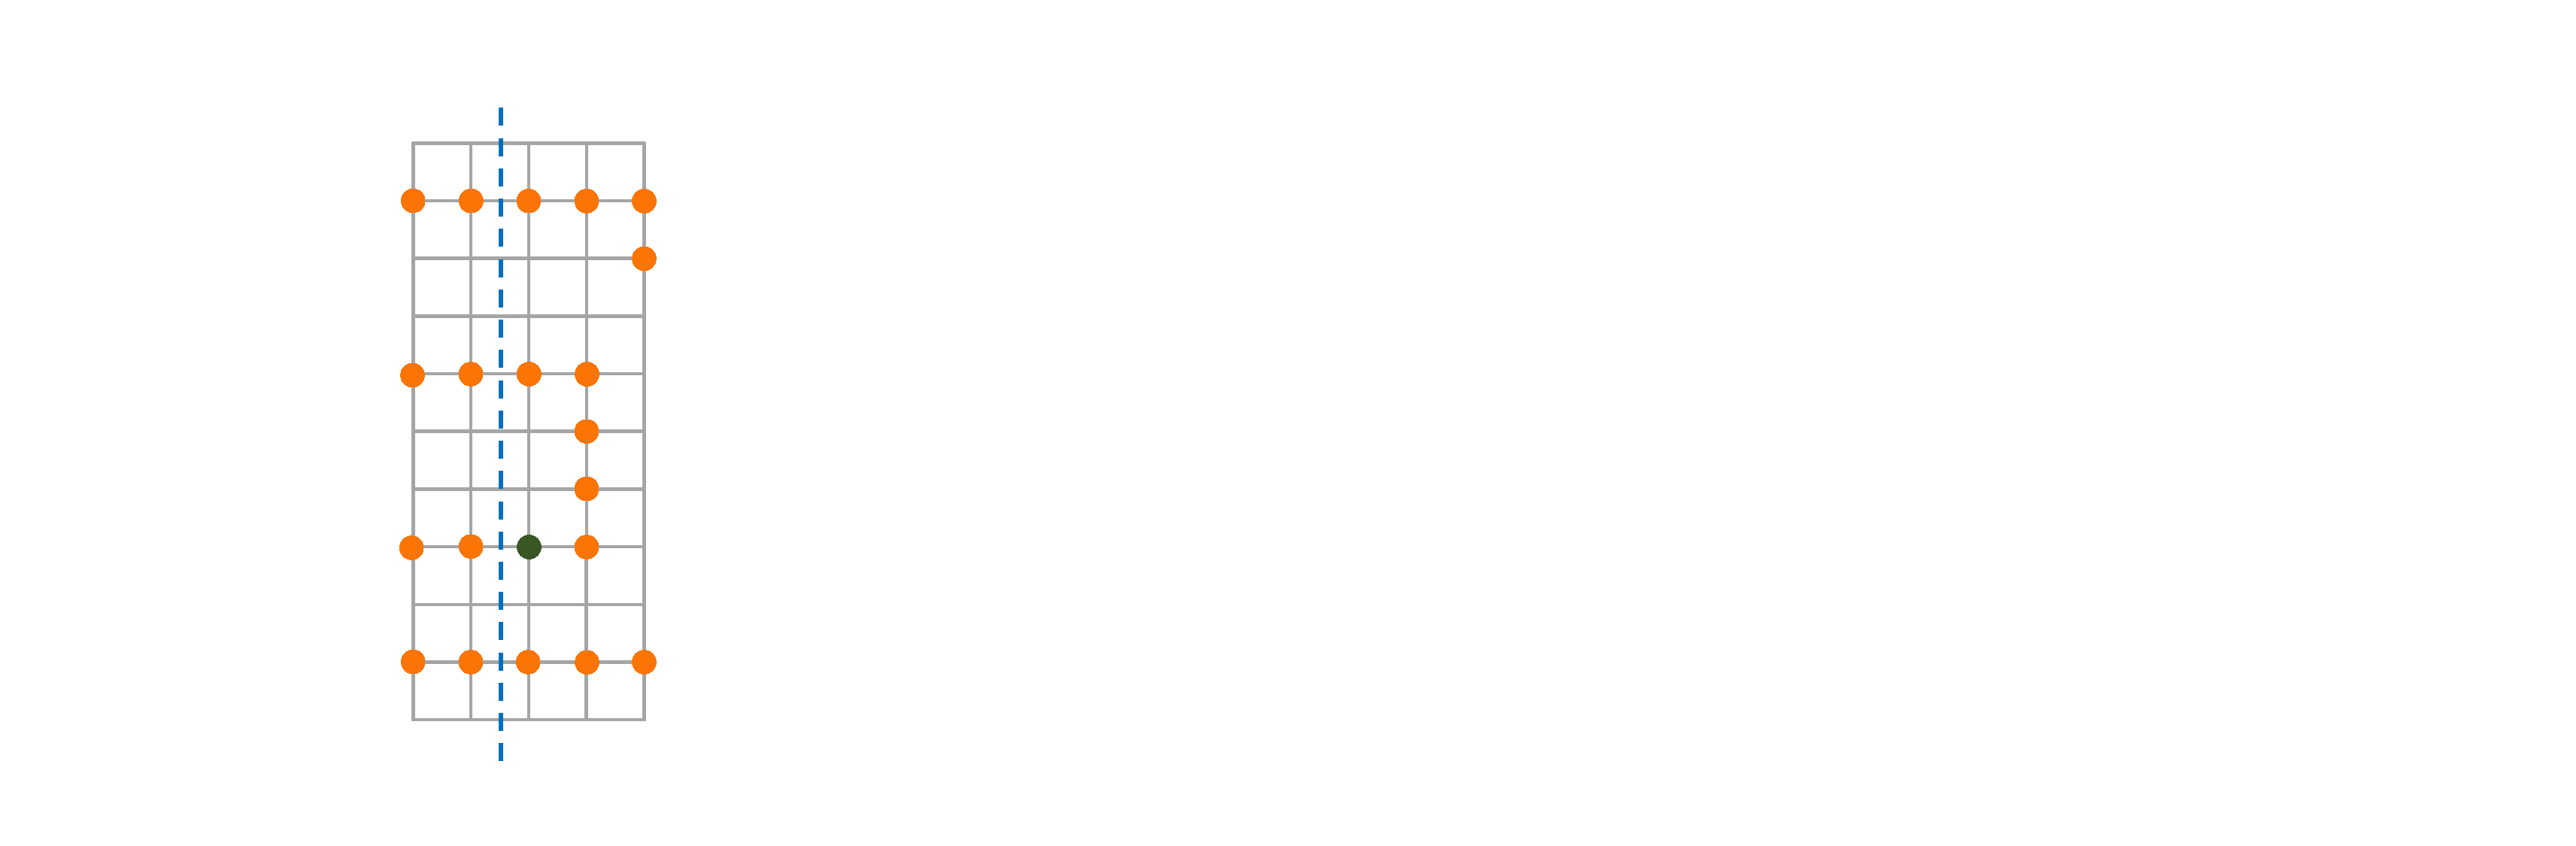
\includegraphics[width = 0.35\linewidth]{pix/sensing-traj/thm4_period.pdf}
\caption{}
\label{fig:thm4_period}
\end{subfigure}
\hfill
\caption{(a) Typical structure of minimum dominating path on the boundary; (b) 2-period coverage and 3-period coverage of specific structure.}
\label{fig:lem2}
\end{minipage}
\hfill
\begin{minipage}{0.6\textwidth}
\begin{subfigure}{0.3\linewidth}
\centering
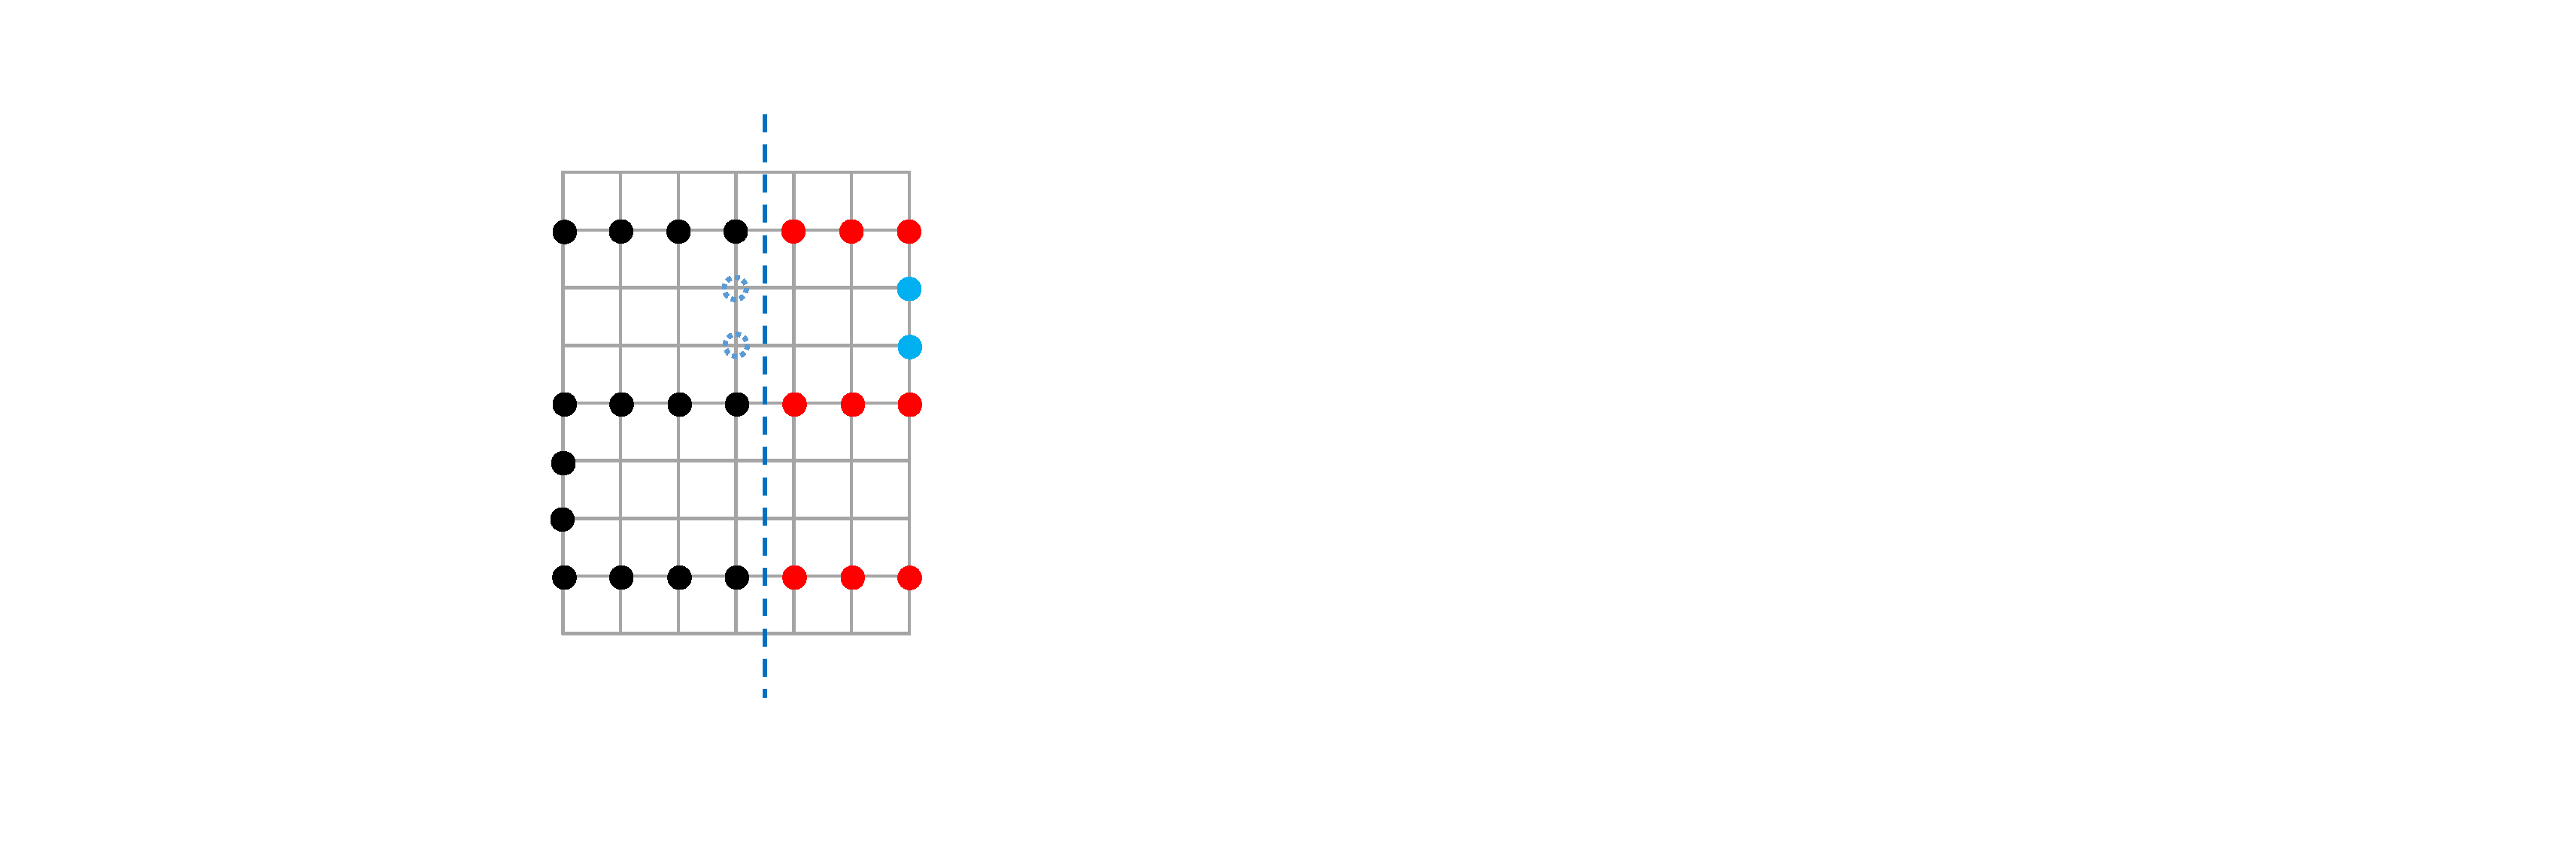
\includegraphics[width = 0.6\linewidth]{pix/sensing-traj/meta_struct1a.pdf}
\caption{The 9$\times$4 grid expanded to the 9$\times$7 grid;}
\vspace{0.15in}
\label{fig:meta_struct1_a}
\end{subfigure}%
\hfill
\begin{subfigure}{0.3\linewidth}
\centering

\includegraphics[width = 0.26\linewidth]{pix/sensing-traj/meta_struct1b.pdf}
\caption{The 13$\times$1 grid expanded to the 13$\times$4 grid;}
\label{fig:meta_struct1_b}
\end{subfigure}
\hfill
\begin{subfigure}{0.3\linewidth}
\centering

\includegraphics[width = 0.22\linewidth]{pix/sensing-traj/meta_struct1c.pdf}
\caption{The 14$\times$1 grid expanded to the 14$\times$4 grid;}
\label{fig:meta_struct1_c}
\end{subfigure}
\caption{Different cases of meta struct 1 by adding $m$ vertices to construct the minimum dominating path in the expanded grid. Red vertices are extra vertices in the minimum dominating path of $L_{m,n+3}$, blue vertices are vertices shifted from blue dashed-line vertices in the $n$-th column, black vertices are part of vertices in the minimum dominating path of $L_{m,n}$. The dashed line separates columns in~$C_{1,n}$ and columns in~$C_{n+1,n+3}$.}
\end{minipage}

\end{figure*}


\subsubsection{Meta structs for constructing the minimum dominating path in $L_{m,n+3}$}
\begin{figure*}
\begin{subfigure}[t]{0.13\textwidth}
\centering

\includegraphics[width=0.75\linewidth]{pix/sensing-traj/meta_struct2a.pdf}
\caption{The 8$\times$4 grid expanded to the 8$\times$7 grid;}
\vspace{0.12in}
\label{fig:meta_struct2_a}
\end{subfigure}%
\hfill
\begin{subfigure}[t]{0.13\textwidth}
\centering
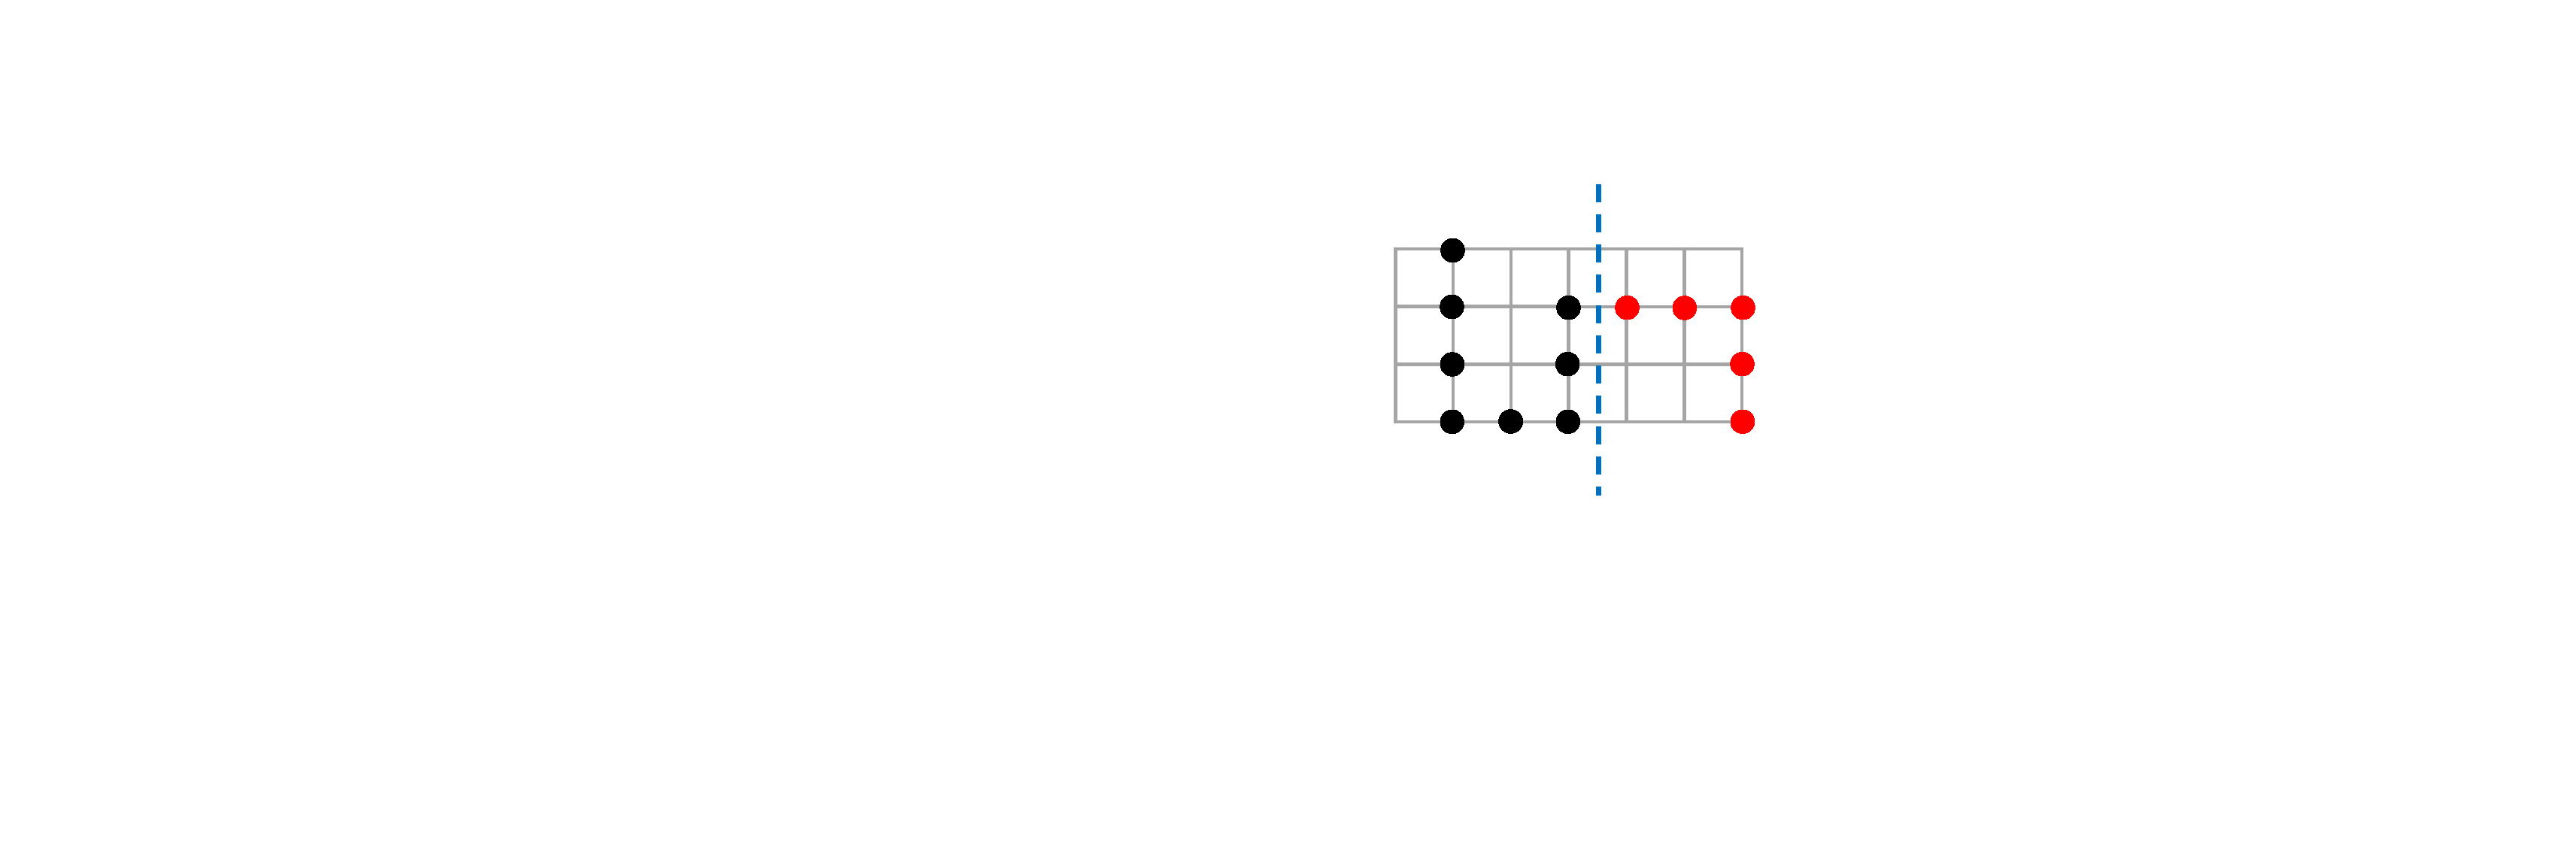
\includegraphics[width=0.8\linewidth]{pix/sensing-traj/meta_struct2b.pdf}
\caption{The 4$\times$4 grid expanded to the 4$\times$7 grid;}
\label{fig:meta_struct2_b}
\end{subfigure}
\hfill
\begin{subfigure}[t]{0.13\textwidth}
\centering
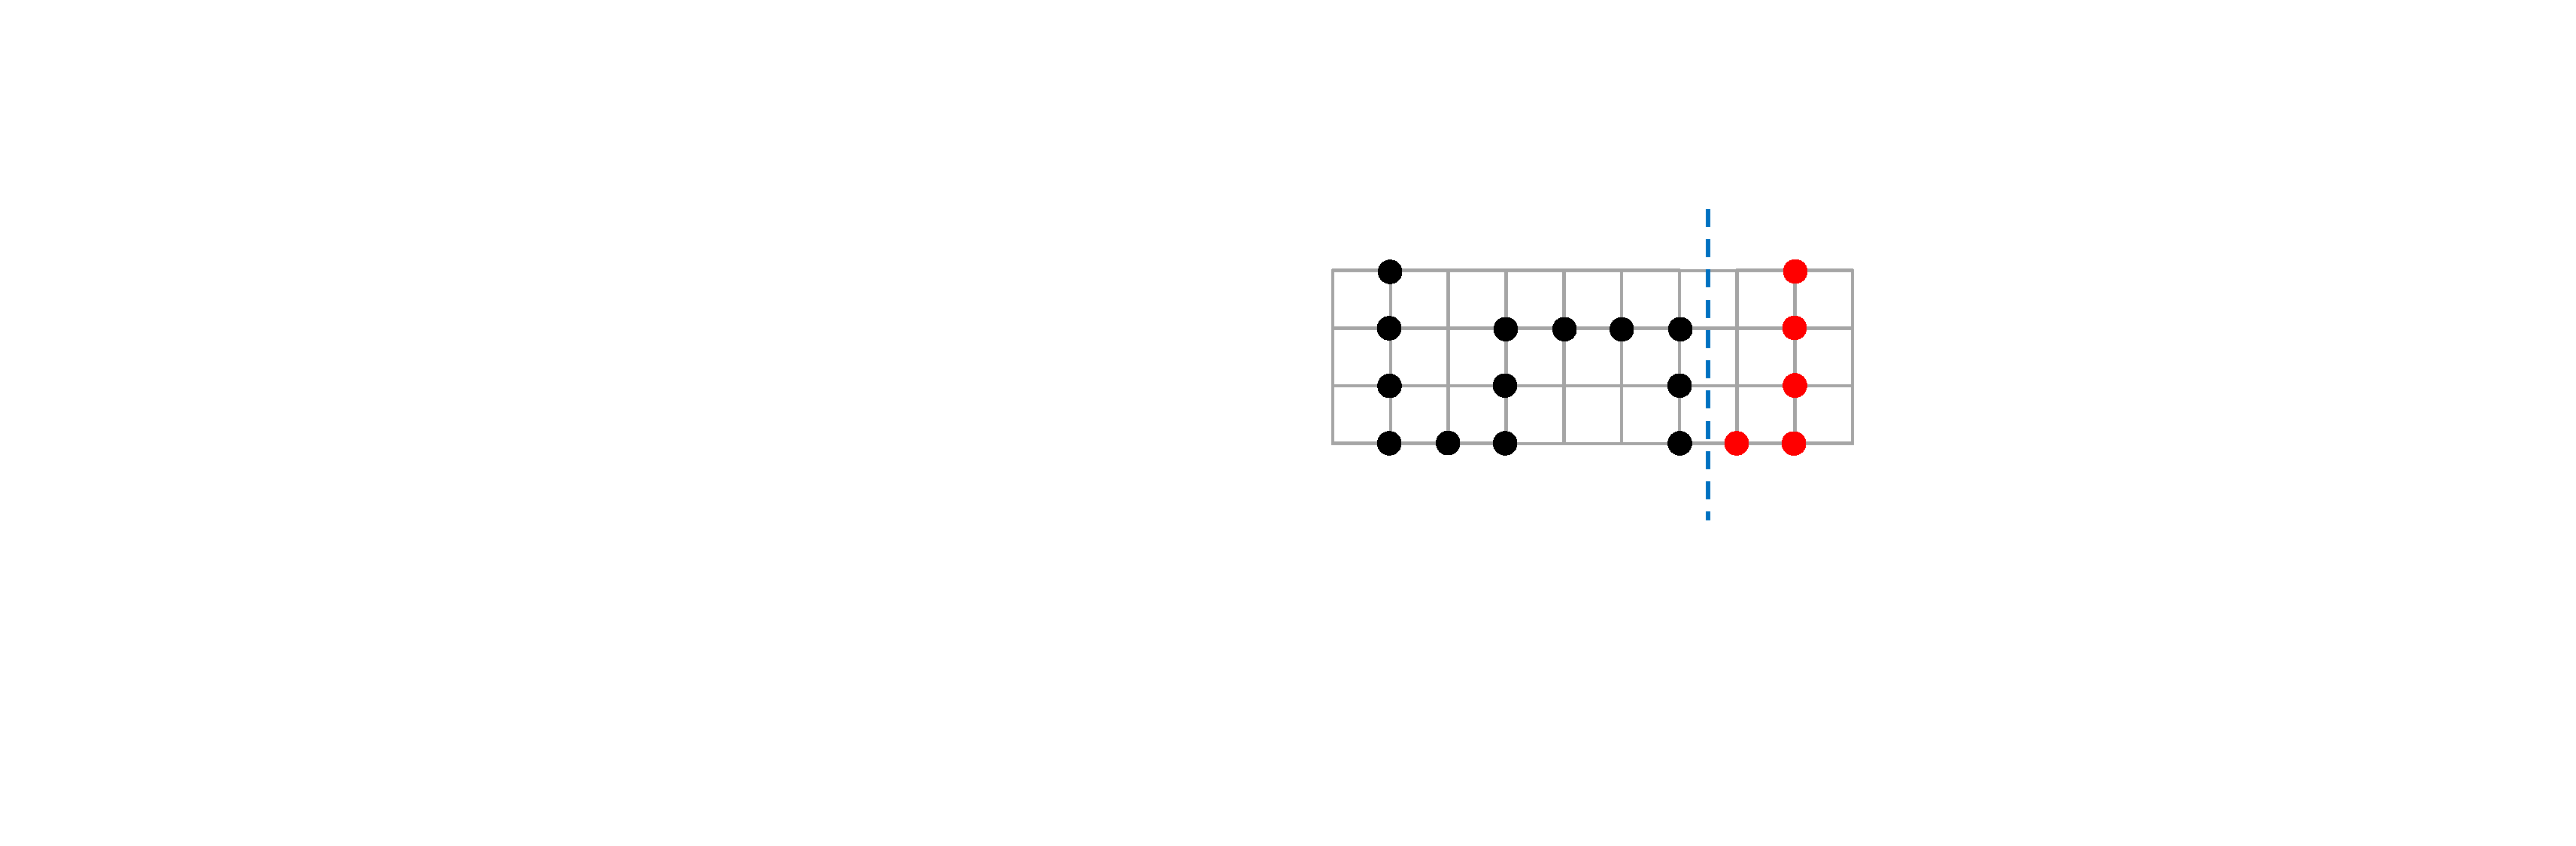
\includegraphics[width=1\linewidth]{pix/sensing-traj/meta_struct2c.pdf}
\caption{The 4$\times$7 grid expanded to the 4$\times$10 grid;}
\label{fig:meta_struct2_c}
\end{subfigure}
\hfill
\begin{subfigure}[t]{0.25\textwidth}
\centering
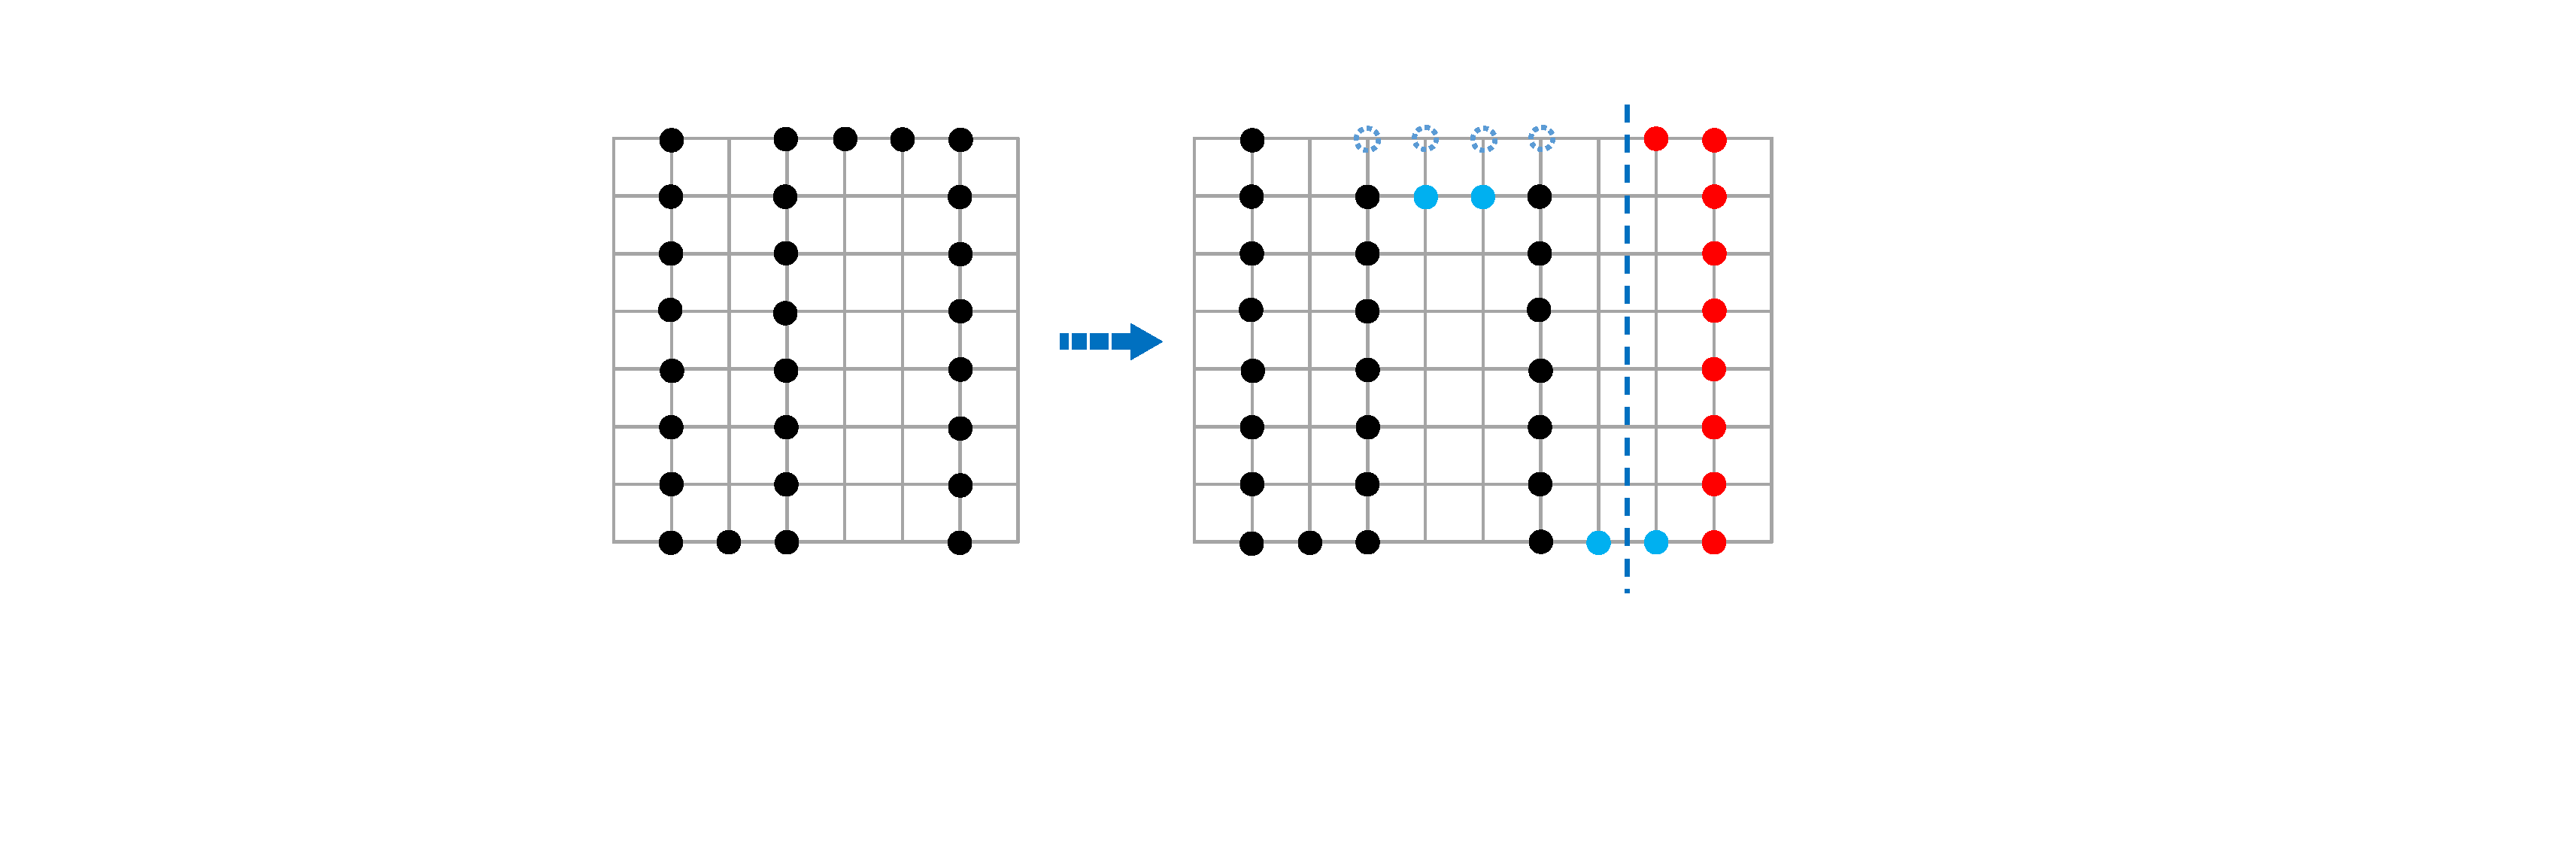
\includegraphics[width=1\linewidth]{pix/sensing-traj/meta_struct2d.pdf}
\caption{The 8$\times$8 grid expanded to the 8$\times$11 grid;}
\label{fig:meta_struct2_d}
\end{subfigure}%
\hfill
\begin{subfigure}[t]{0.2\textwidth}
\centering
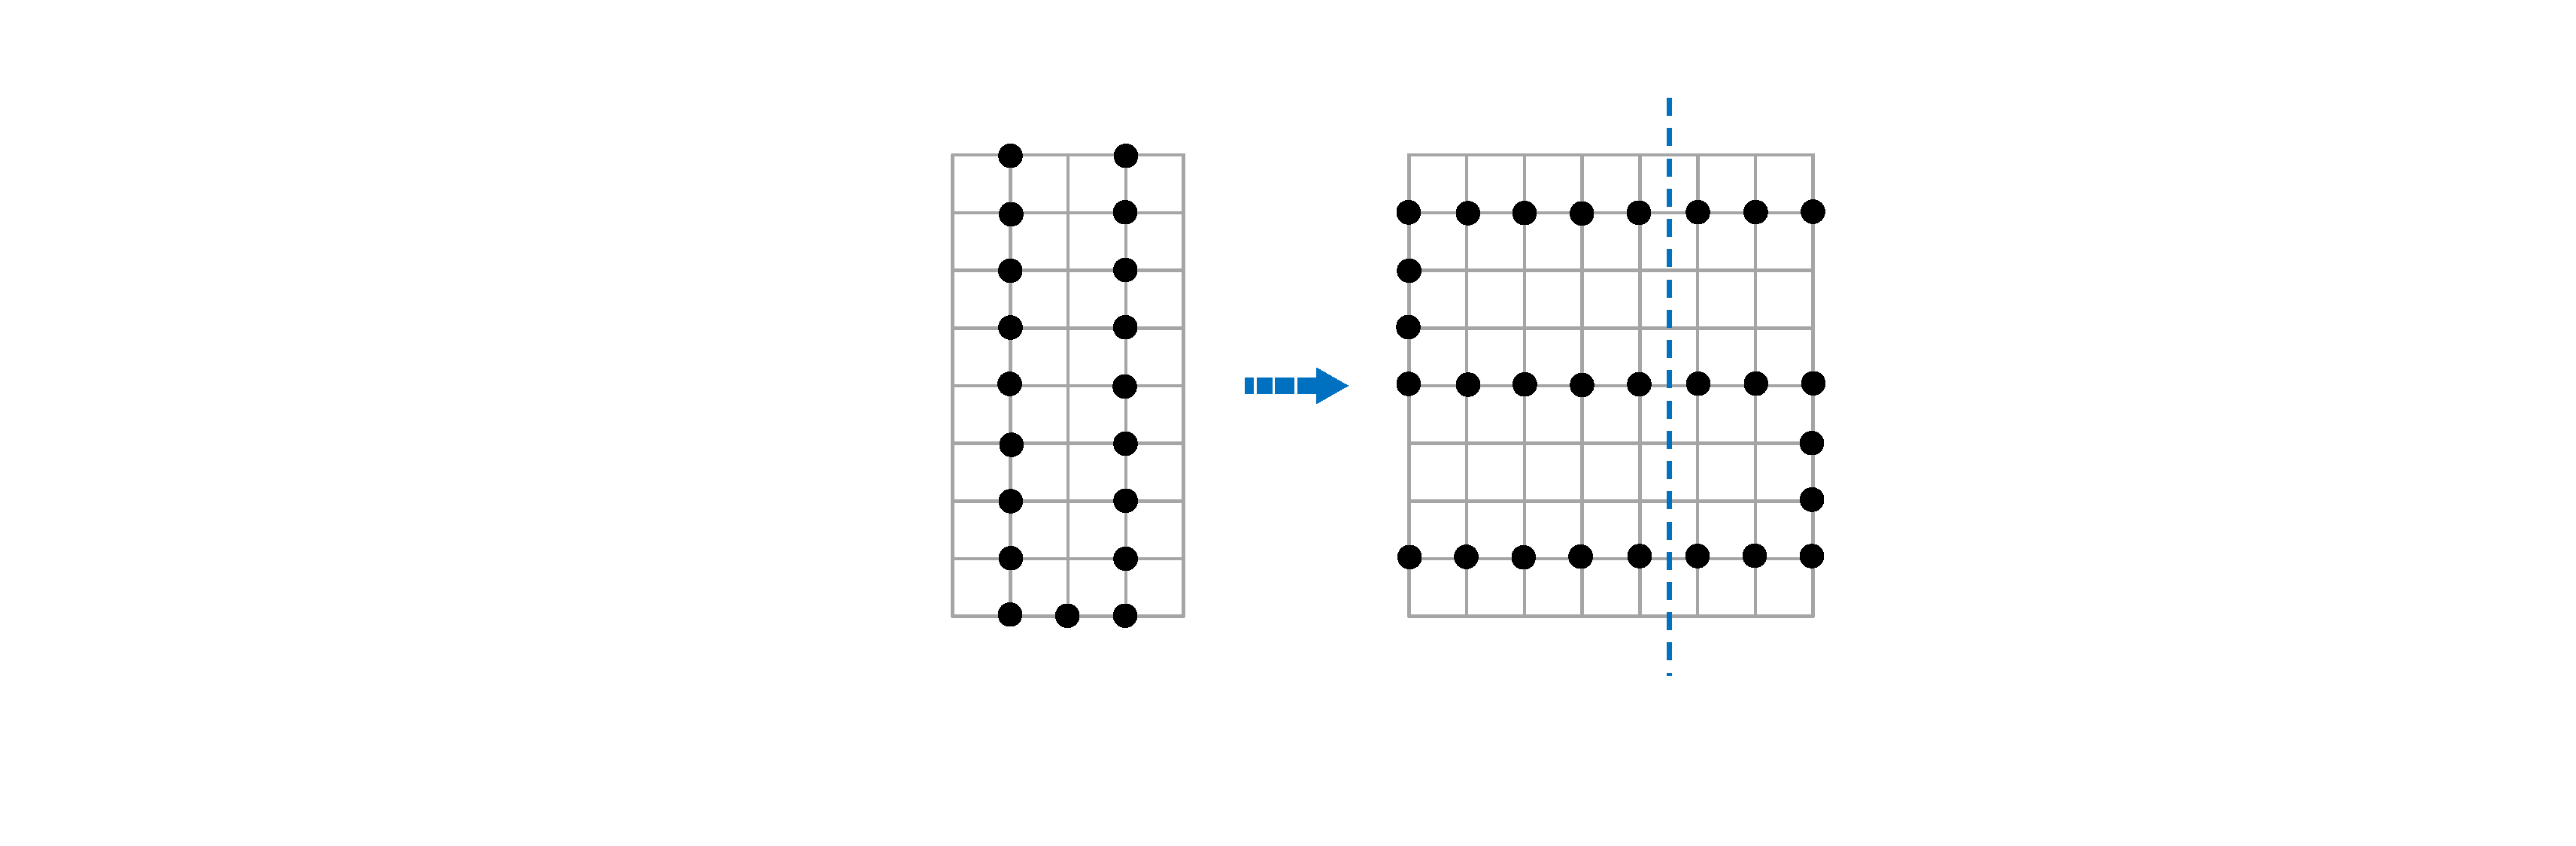
\includegraphics[width=0.9\linewidth]{pix/sensing-traj/meta_struct2e.pdf}
\caption{The 9$\times$5 grid expanded to the 9$\times$8 grid;}
\label{fig:meta_struct2_e}
\end{subfigure}
\hfill
\caption{Different cases of meta struct 2 by adding $(m+1)$ vertices to construct the minimum dominating path in the expanded grid.}
\end{figure*}

\begin{figure*}[htbp]
\begin{minipage}[t]{0.23\linewidth}
 \centering
 
\includegraphics[width=0.4\linewidth]{pix/sensing-traj/meta_struct3.pdf}
\caption{An example of meta struct 3 when expanding a 5$\times$3 grid to a 5$\times$6 one.}
\label{fig:meta_struct3}
\end{minipage}
\hfill
 \begin{minipage}[t]{0.23\linewidth}
 \centering
 
\includegraphics[width=0.9\linewidth]{pix/sensing-traj/path_case_1.pdf}
 \caption{The minimum dominating path for $L_{1,4}$, $L_{2,4}$ and $L_{3,4}$ }
\label{fig:path_case_1}
\end{minipage}
\hfill
\begin{minipage}[t]{0.23\linewidth}
\centering
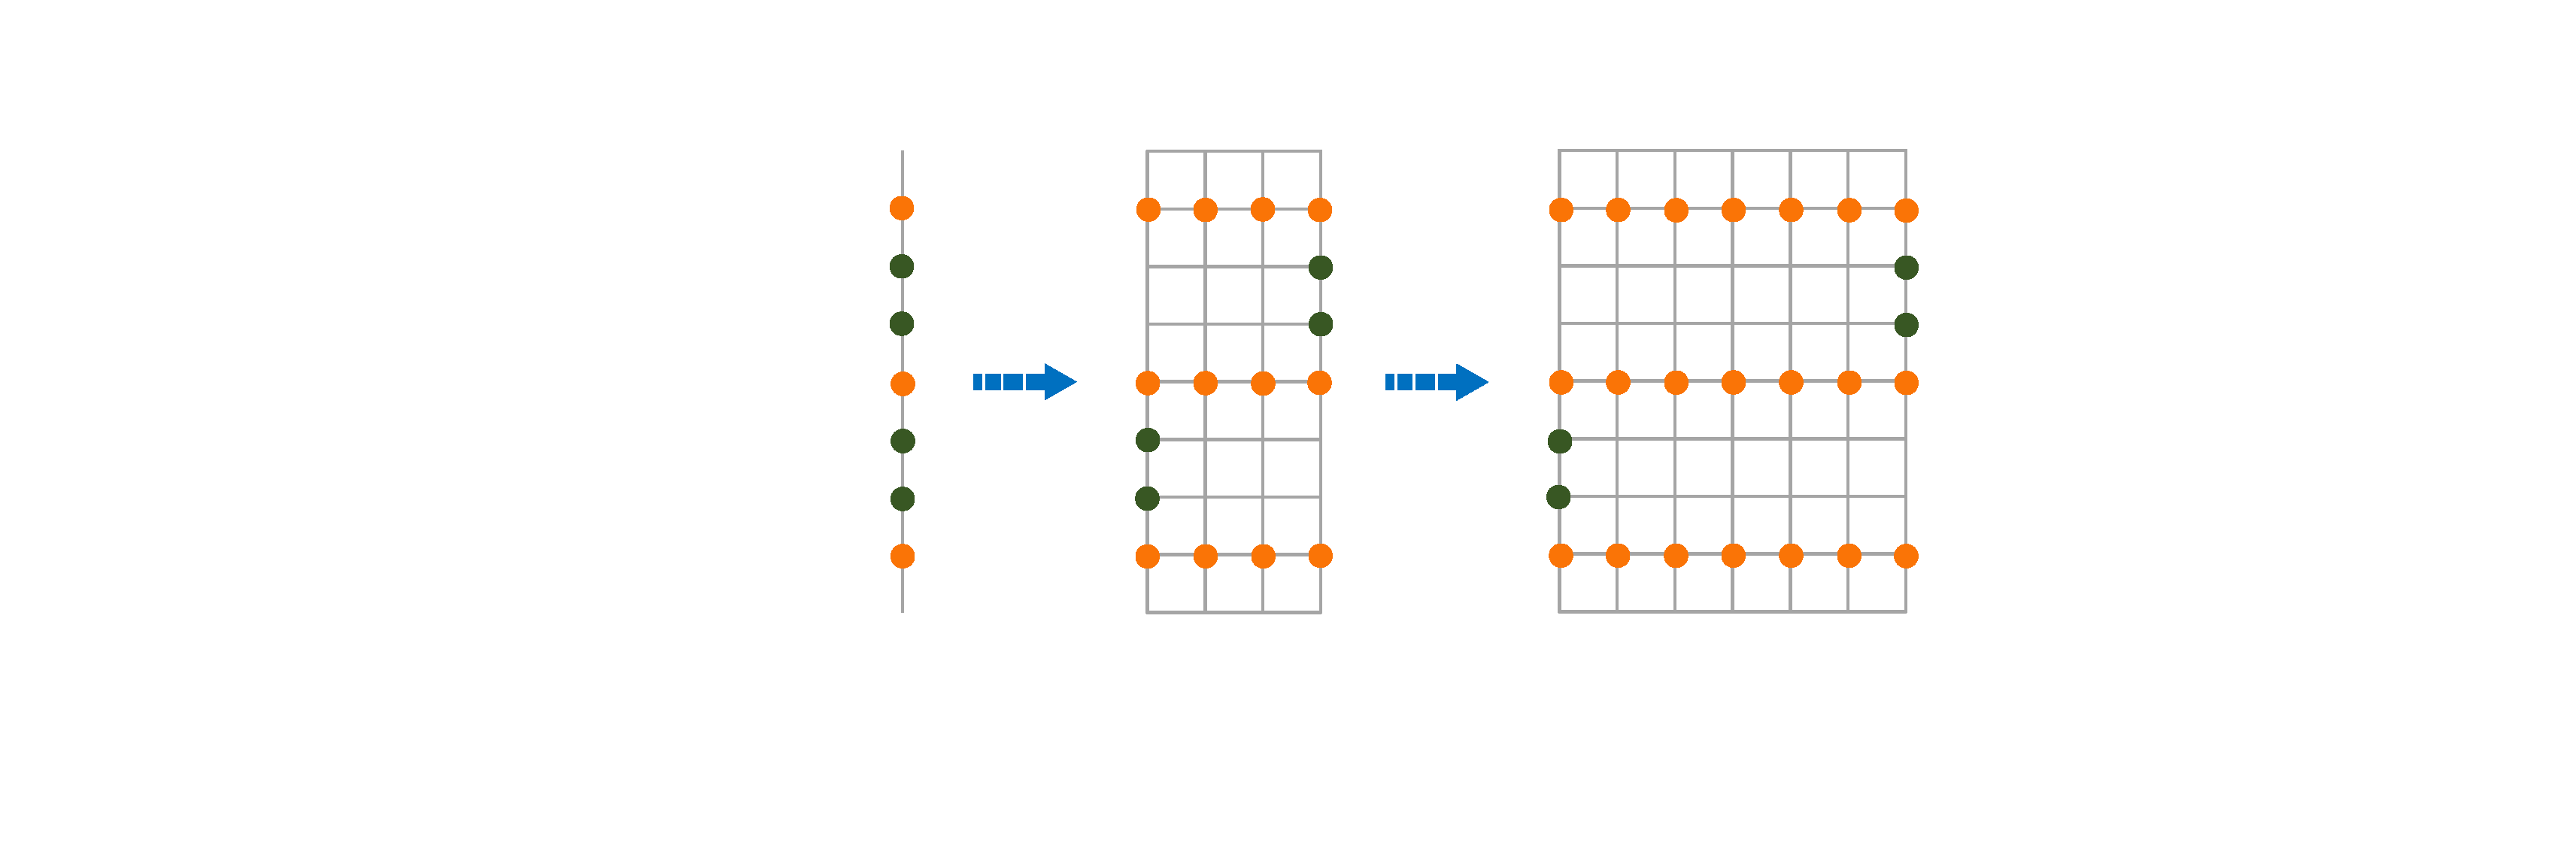
\includegraphics[width=0.9\linewidth]{pix/sensing-traj/path_case_2_1.pdf}
\caption{Minimum dominating path when $m \equiv 0 \pmod 3$, $n \equiv 1 \pmod 3$.}
\label{fig:path_case_2_1}
\end{minipage}%
\hfill
\begin{minipage}[t]{0.23\linewidth}
\centering
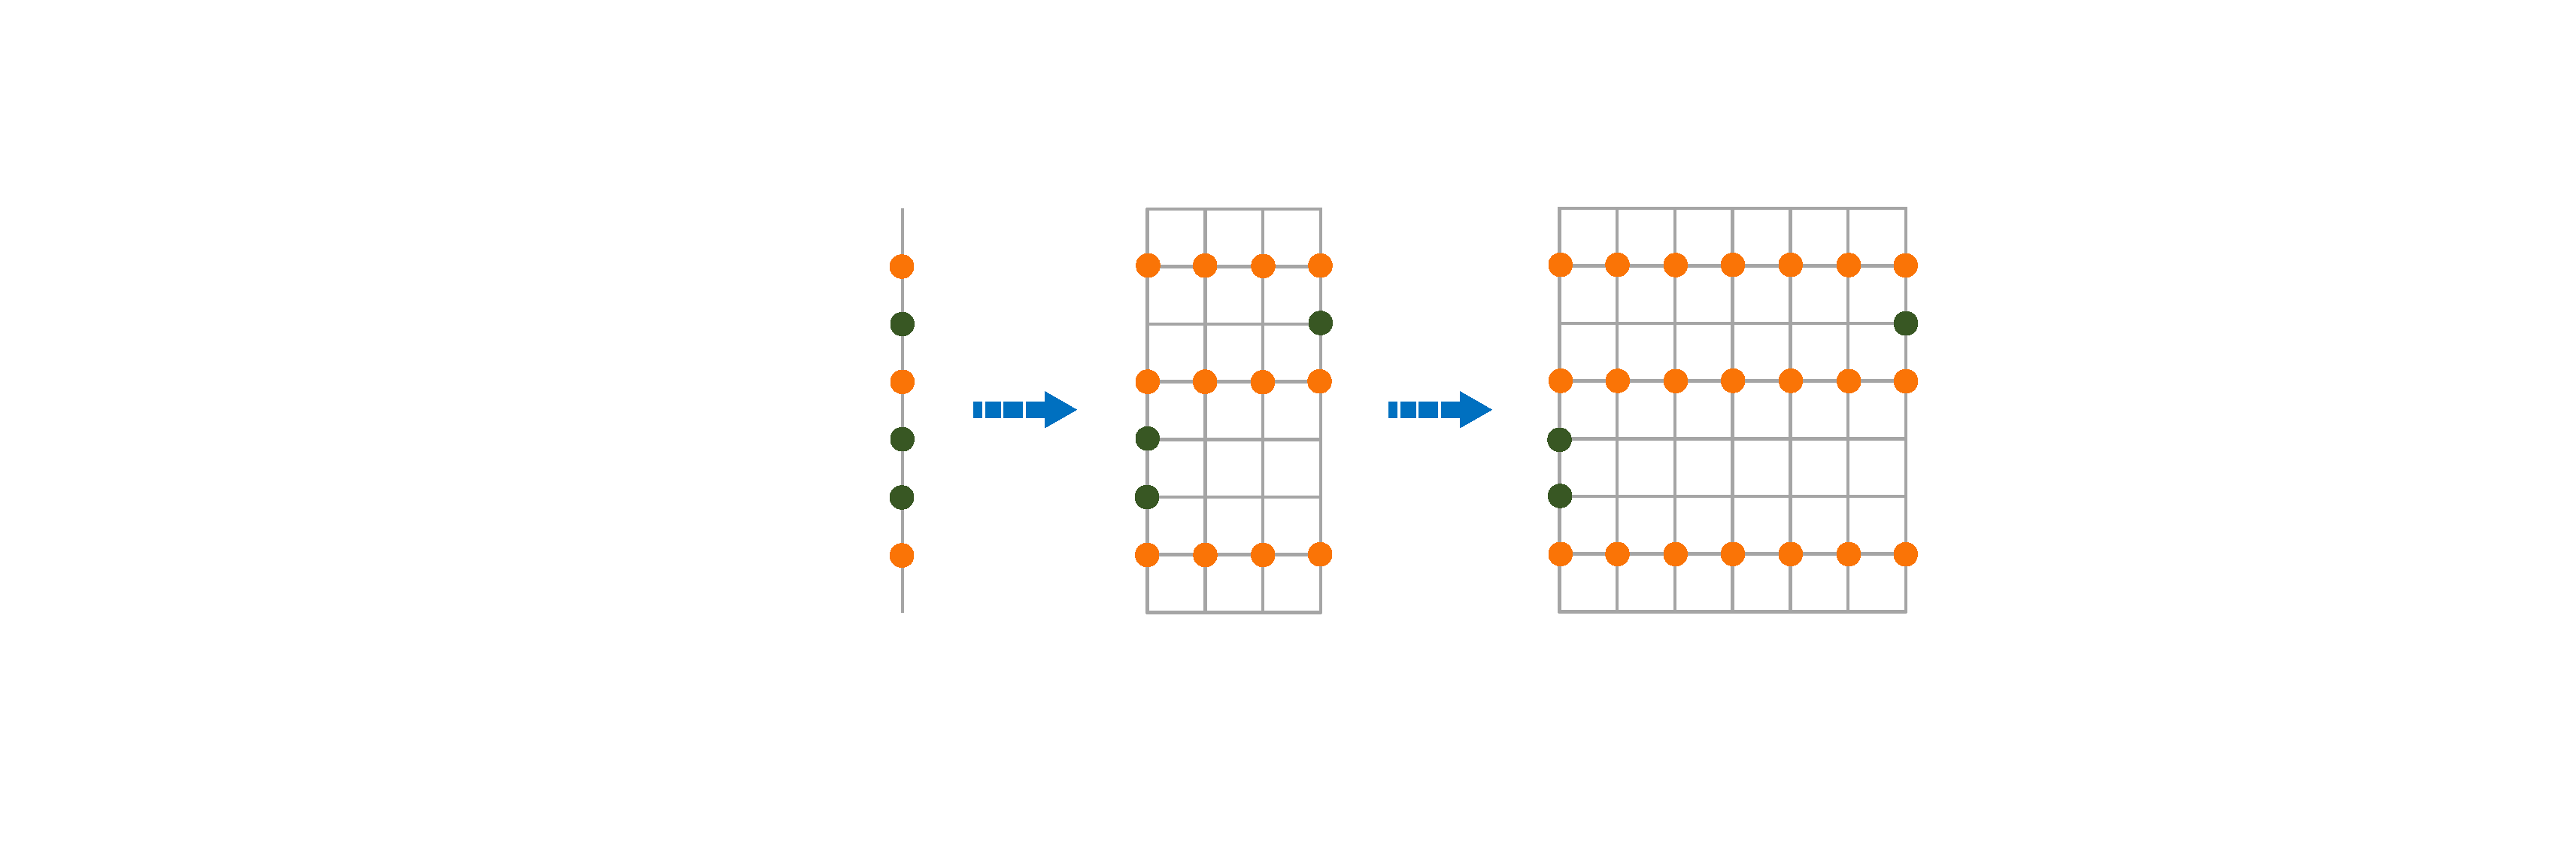
\includegraphics[width=0.9\linewidth]{pix/sensing-traj/path_case_2_2.pdf}
\caption{Minimum dominating path when $m \equiv 2 \pmod 3$, $n \equiv 1 \pmod 3$.}
\label{fig:path_case_2_2}
\end{minipage}
\end{figure*}

In Theorem~\ref{thm:3period}, we have proofed the minimum number of vertices needed to add into the minimum dominating path in $L_{m,n}$ to construct minimum dominating path of $L_{m,n+3}$ is $m$, which can be achieved in certain structures of the grid. In other structures, we need either $(m+1)$ or $(m+2)$ vertices to construct the minimum dominating path in $L_{m,n+3}$ from that in $L_{m,n}$.
We call these certain structures in grids as three types of \emph{meta struct}.

\textbf{Struct~1: $\gamma_p(L_{m,n+3})-\gamma_p(L_{m,n})=m$}. There are two cases for meta struct 1.
\begin{enumerate}
  \item When $m \equiv 0 \pmod 3$, we could select vertices (red ones in Figure~\ref{fig:meta_struct1_a}) in rows~$r_2$, $r_5$..., $r_m-1$ in columns in~$C_{n+1,n+3}$ into minimum dominating path, plus the vertices (blue ones in Figure~\ref{fig:meta_struct1_a}) shifted from column~$c_n$ to column~$c_{n+3}$, as shown in Figure~\ref{fig:meta_struct1_a}. This struct can be repeated in bigger-size grids.
  \item When $n=1$, when $m \equiv 3 \pmod 1$ we could construct as Figure~\ref{fig:meta_struct1_b} and when $m \equiv 3 \pmod 2$ we could construct as Figure~\ref{fig:meta_struct1_c}. Both cases could only exist once.
\end{enumerate}





\textbf{Struct~2: $\gamma_p(L_{m,n+3})-\gamma_p(L_{m,n})=m+1$}. There are five cases for meta struct 2.
\begin{enumerate}
  \item When $m \equiv 2 \pmod 3$, we could construct the minimum dominating path using struct as shown in Figure~\ref{fig:meta_struct2_a}, which can be also repeated in bigger-size grids.
  \item When $c_n \setminus v_{1,n}$ belongs to minimum dominating path in $L_{m,n}$, we have another meta struct as shown in  Figure~\ref{fig:meta_struct2_b}.
  \item When $v_{1,n}$ belongs to the minimum dominating path in $L_{m,n}$, we have the meta struct as shown in Figure~\ref{fig:meta_struct2_c}.
  \item When $n \equiv 2 \pmod 3$ and $n \geq 8$, we could use the meta struct as shown in Figure~\ref{fig:meta_struct2_d} to construct the minimum dominating path in $L_{m,n+3}$.
  \item When $n \equiv 0 \pmod 3$, we could rotate direction of minimum dominating path of $L_{m,n}$ and construct with meta struct~1. If the rotation only brings one extra vertex, we have the meta struct as shown in Figure~\ref{fig:meta_struct2_e}.
\end{enumerate}


\textbf{Struct~3: $\gamma_p(L_{m,n+3})-\gamma_p(L_{m,n})=m+2$}.
There are many cases for meta struct 3, and we only show the most common case here.
When there are no vertices in column~$c_n$ that belong to the minimum dominating path $P^*$ in $L_{m,n}$, vertices in $c_{n-1}$ must belong to $P^*$. Then, we could construct the minimum dominating path $P$ in $L_{m,n+3}$ with the meta struct as shown in Figure~\ref{fig:meta_struct3}, by adding $(m+2)$ vertices (red ones in Figure~\ref{fig:meta_struct3}).




\subsection{Trajectory planning based on meta structs}\label{sec:floating}
Based on the previous meta structs, we will elaborate the trajectory planning procedure in the following---i.e., construct the minimum dominating path $P$ in grid $L_{m,n}$: (1) $m<4$ and $m<n$; (2) $m \equiv 0 \pmod 3$, $n \equiv 1 \pmod 3$ or $m \equiv 2 \pmod 3$, $n \equiv 1 \pmod 3$; (3) $m \equiv 0 \pmod 3$, $n \equiv 0 \pmod 3$ or $m \equiv 0 \pmod 3$, $n \equiv 2 \pmod 3$ or $m \equiv 2 \pmod 3$, $n \equiv 2 \pmod 3$; and (4) $m \equiv 1 \pmod 3$, $n \equiv 1 \pmod 3$.



\subsubsection{Case~1}
In trivial cases when $m<4$ and $m<n$, since the connected dominating set is also dominating path, we have the same structure as shown in Figure~\ref{fig:path_case_1} of \cite{Hamburger2007Routing}.
Therefore, we have
\begin{enumerate}
  \item $\gamma_p(L_{1,1})=\gamma_p(L_{1,2})=1$, and if $3 \leq n$, $\gamma_p(L_{1,n})=n-2$
  \item $\gamma_p(L_{2,2})=\gamma_p(L_{2,3})=2$, and if $4 \leq n$, $\gamma_p(L_{2,n})=n$
  \item $\gamma_p(L_{3,n})=n$
\end{enumerate}


\subsubsection{Case~2}
Since the minimum dominating path in $L_{m,1}$ contains $m-2-\lceil \frac{m}{3} \rceil$ connecting vertices, when $m \equiv 0 \pmod 3$ and $n \equiv 1 \pmod 3$, we could use the meta struct~1-1) to construct $L_{m,n}$, and we can construct the minimum dominating path as shown in Figure~\ref{fig:path_case_2_1}. Therefore, when $m \equiv 0 \pmod 3$, $n \equiv 1 \pmod 3$, we have $\gamma_p(L_{m,n})=3ab+3a-2$.

Similarly, when $m \equiv 2 \pmod 3$, $n \equiv 1 \pmod 3$, if $m \geq 11$, we use meta struct~1-3) when $n=1$, then we use meta struct~2-1) as $n$ increases. And when $m \equiv 2 \pmod 3$, $n \equiv 1 \pmod 3$, if $m<11$, we use meta struct~2-1) to construct the minimum dominating path, as shown in Figure~\ref{fig:path_case_2_2}.
Therefore, when $m \equiv 2 \pmod 3$, $n \equiv 1 \pmod 3$, we have
\[
\gamma_p(L_{m,n})=\left\{
\begin{array}{rcl}
3ab+3a+3b       &      & {a \leq 2}\\
3ab+3a+3b-1       &      & {otherwise}.
\end{array} \right.
\]


\begin{figure*}
\begin{minipage}[t]{0.32\textwidth}
\centering
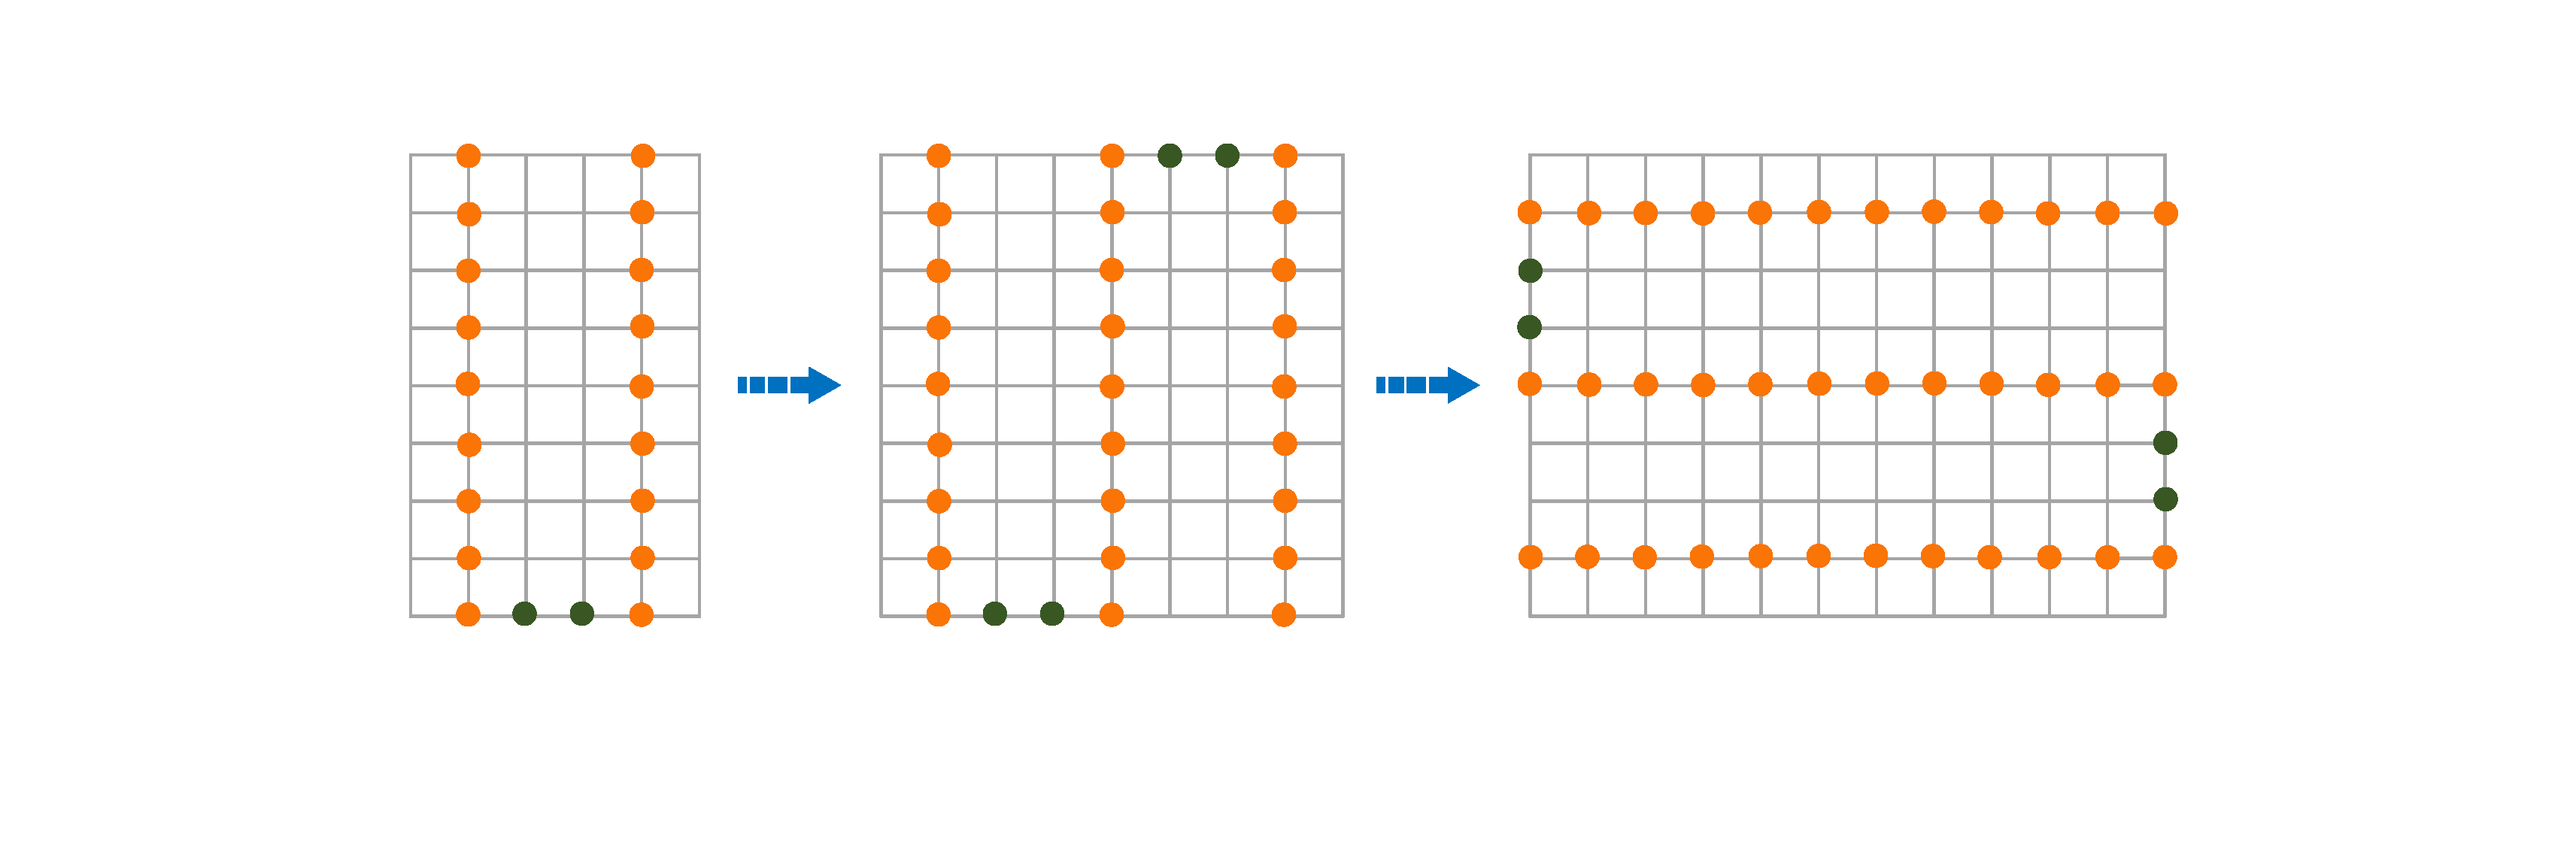
\includegraphics[width=1.0\linewidth]{pix/sensing-traj/path_case_3_1.pdf}
\caption{Minimum dominating path when $m \equiv 0 \pmod 3$, $n \equiv 0 \pmod 3$.}
\label{fig:path_case_3_1}
\end{minipage}%
\hfill
\begin{minipage}[t]{0.32\textwidth}
\centering
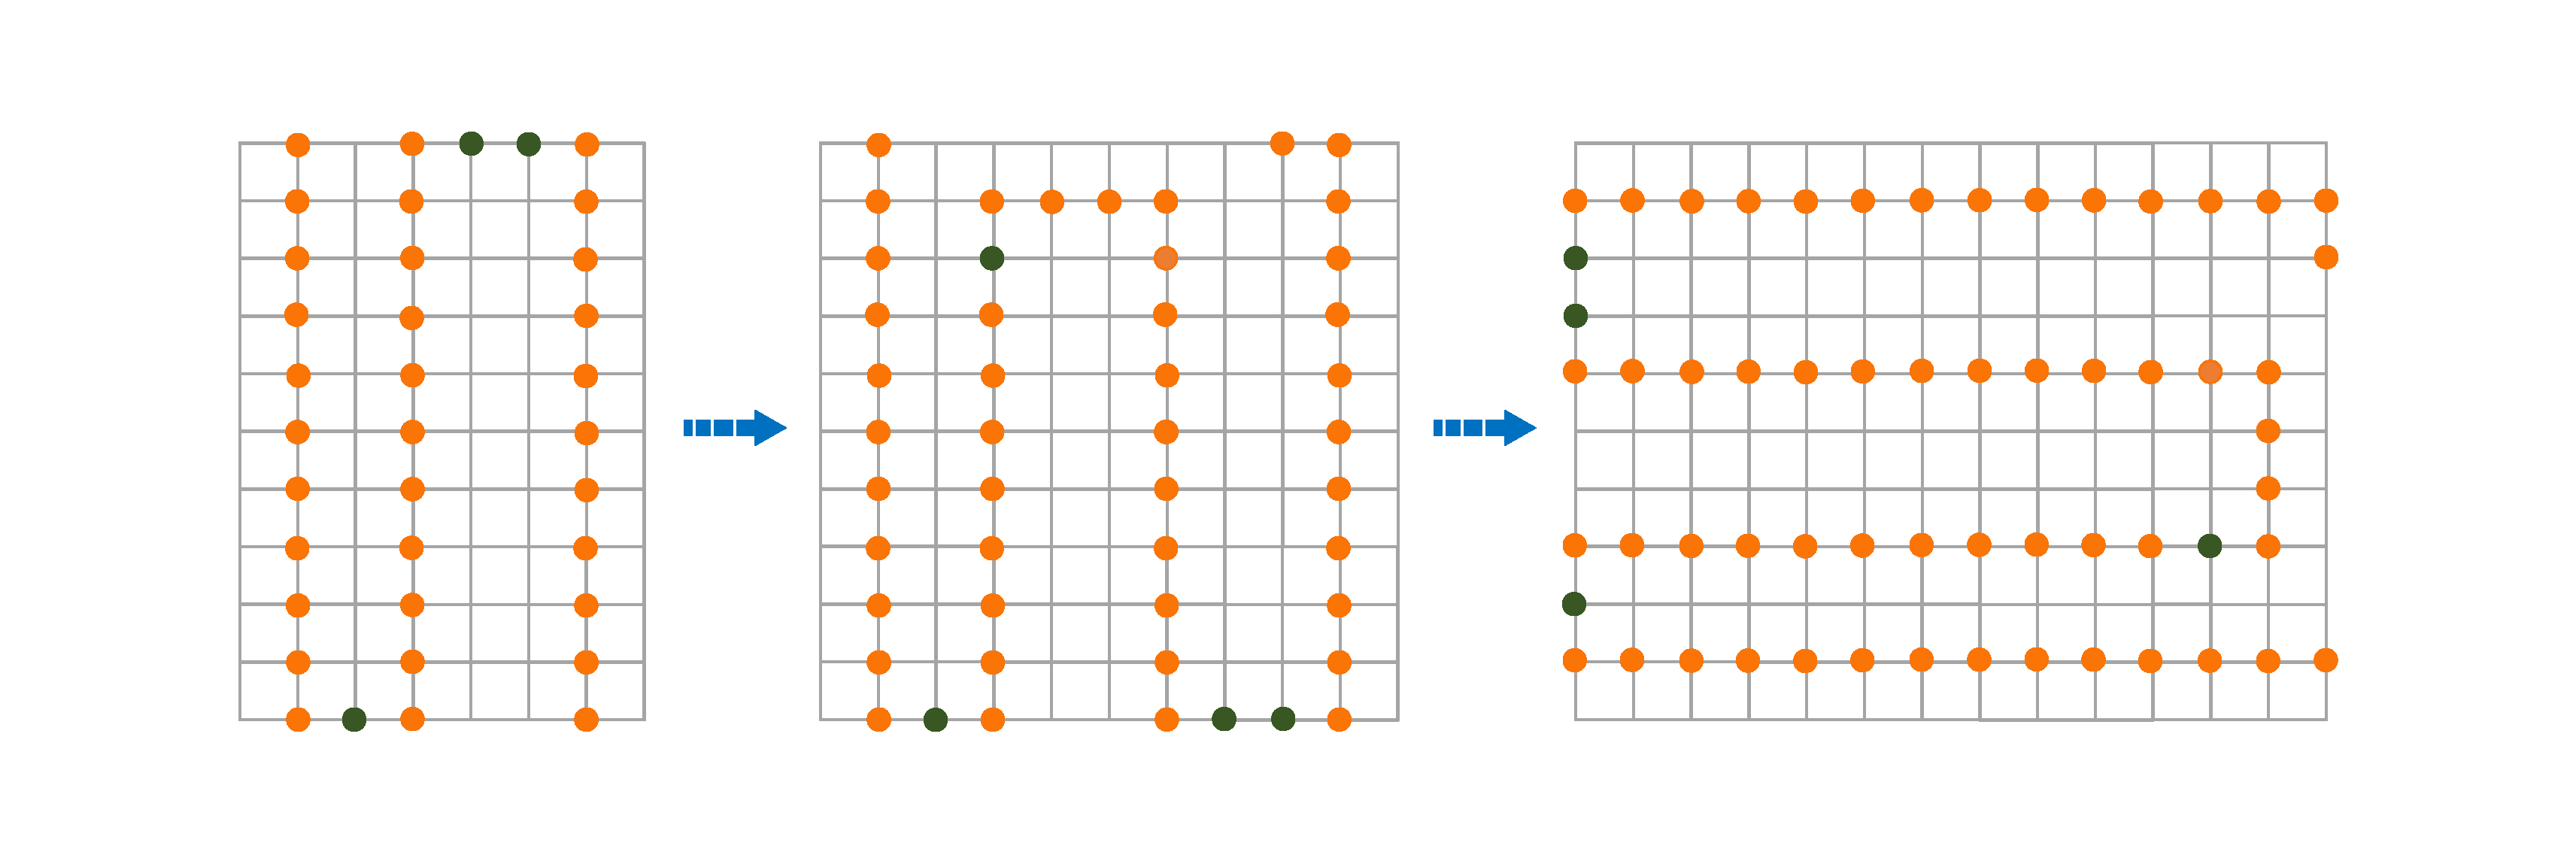
\includegraphics[width=1.0\linewidth]{pix/sensing-traj/path_case_3_2.pdf}
\caption{Minimum dominating path when $m \equiv 2 \pmod 3$, $n \equiv 2 \pmod 3$.}
\label{fig:path_case_3_2}
\end{minipage}
\hfill
\begin{minipage}[t]{0.32\textwidth}
\centering
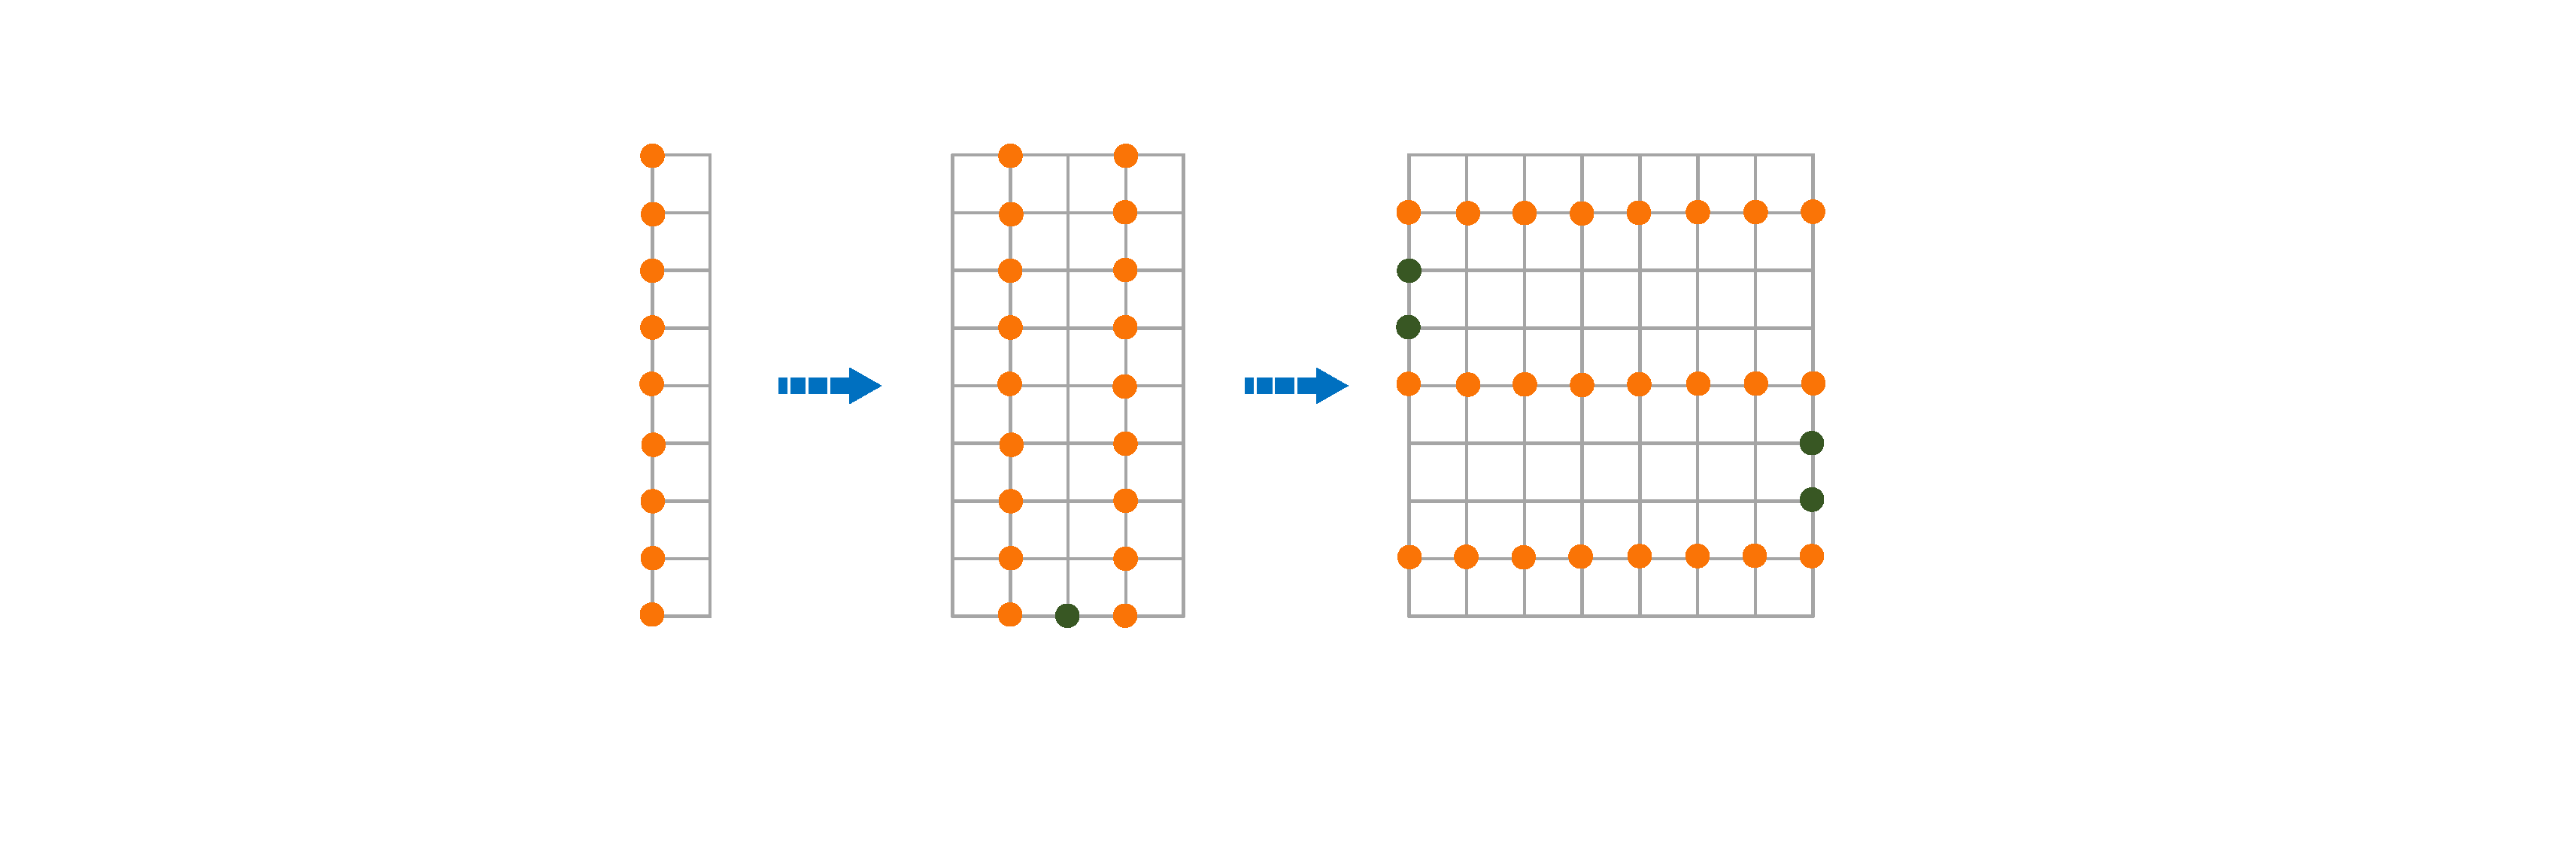
\includegraphics[width=0.7\linewidth]{pix/sensing-traj/path_case_3_3.pdf}
\caption{Minimum dominating path when $m \equiv 0 \pmod 3$, $n \equiv 2 \pmod 3$.}
\label{fig:path_case_3_3}
\end{minipage}
\end{figure*}

\subsubsection{Case~3}
We use the induction on the structure to construct the minimum dominating path of $L_{m,n}$ in this case.

When $m \equiv 0 \pmod 3$, $n \equiv 0 \pmod 3$, if $m=6$, we could construct $L_{6,n}$ using meta struct~1-1). Assume the result holds for $m=k$, then we could get the minimum dominating path for $L_{k+3,k}$ from $L_{k,k+3}$, since none of meta struct~1 or meta struct~2 will fit in the structure, we could use meta struct~3 to get the minimum dominating path for $L_{k+3,k+3}$. Then, we could use meta struct~1-1) to get $L_{k+3,n}$ when $n \geq k+3$ as shown in Figure~\ref{fig:path_case_3_1} which holds the structure for $k+3$. We could use the same approach to construct minimum dominating path, when $m \equiv 2 \pmod 3$, $n \equiv 2 \pmod 3$ as shown in Figure~\ref{fig:path_case_3_2}.

When $m \equiv 0 \pmod 3$, $n \equiv 2 \pmod 3$, we have two structures (a) and (b) as shown in Figure~\ref{fig:path_case_3_3} and for different $n$ we also have two structures shown in Figure~\ref{fig:path_case_3_2}. Assume the result holds for $m=k$, and the critical point between structure (a) and structure (b) is $n=l$ when $m=k$. Specifically, when $n \leq l$, $L_{k,n}$ has structure (a) and otherwise, $L_{k,n}$ has structure (b). For $L_{k,n}$ with structure (a), we could use meta struct~2-1) to construct minimum dominating path of $L_{k+3, l}$. Since structure (a) could only use meta struct~3 or meta struct~2-5) to extend columns, we use meta struct~3 on $L_{k+3,l}$ until it satisfies the condition of meta struct~2-5) which could rotate the direction. Therefore, we could hold result for $m=k+3$.

Therefore, we have following results.

When $m \equiv 0 \pmod 3$, $n \equiv 0 \pmod 3$, assume $m \leq n$, we have $\gamma_p(L_{m,n})=3ab+2a-2$.
When $m \equiv 2 \pmod 3$, $n \equiv 2 \pmod 3$, assume $m \leq n$, we have
\[
\gamma_p(L_{m,n})=\left\{
\begin{array}{rcl}
3ab+4a+3b+1       &      & {a \leq 2}\\
3ab+4a+3b      &      & {otherwise.}
\end{array} \right.
\]
When $m \equiv 0 \pmod 3$, $n \equiv 2 \pmod 3$, we have
\[
\gamma_p(L_{m,n})=\left\{
\begin{array}{rcl}
3ab+3a-1+\min\{a-1, 2b\}       &      & {b \leq 2}\\
3ab+3a-2+\min\{a, 2b\}       &      & {otherwise.}
\end{array} \right.
\]


\subsubsection{Case~4}
We could easily get the minimum dominating path of $L_{4,4}$ in Figure~\ref{fig:path_case_4}. Therefore, we use meta struct~2-2) to construct the minimum dominating path of $L_{4,7}$ and we use meta~struct~2-3) to construct the minimum dominating path of $L_{7,7}$. Besides, we construct minimum dominating path of $L_{4,n}$ when $n \geq 10$ from $L_{1,n}$ with a meta struct~1-2). Finally, for $m \geq 7$, $n \geq 10$, we could only use meta struct 3 to construct the minimum dominating path of $L_{m,n}$ from $L_{m-3,n}$, which leads to the result in Figure~\ref{fig:path_case_4}.

Therefore, when $m \equiv 1 \pmod 3$, $n \equiv 1 \pmod 3$, we have
\[
\gamma_p(L_{m,n})=\left\{
\begin{array}{rcl}
3ab+3a+3b-3       &      & {a+b \leq 4}\\
3ab+2a+2b+1       &      & {otherwise.}
\end{array} \right.
\]

%\begin{algorithm}[htb]
%\caption{Trajectory planning for UAV in 2D grids when considering flight time only.}
%\label{alg:Framwork1}
%\begin{algorithmic}[1]
%\Require
%The graph of trajectory planning, $L_{m,n}$;
%The length of grid, $m$;
%The width of gird, $n$;
%\Ensure
%The trajectory of two-dimensional coordinate of grid, $V_P$;
%\label{code:fram:calculateab}
%\State $a=\lfloor \frac{m}{3} \rfloor$, $b=\lfloor \frac{m}{3} \rfloor$, $ra \equiv m \pmod 3$, $rb \equiv n \pmod 3$;
%
%\label{code:fram:judgemod}
%\If{$(ra=1$ and $rb=0)$ or $(ra=1$ and $rb=2)$ or $(ra=0$ and $rb=2$ and $a>2b)$ or $(ra=2$ and $rb=0$ and $b \leq 2a)$ or $(ra \equiv rb \pmod 3$ and $a>b)$}
%\State swap($m$, $n$), swap($a$, $b$), swap($ra$, $rb$);
%\EndIf
%
%\label{code:fram:calculate}
%\If{$m<4$ or $n<4$}
%    \If{$m>n$}
%        \State swap($m$, $n$), swap($a$, $b$), swap($ra$, $rb$);
%    \EndIf
%
%    \If{$m=1$}
%        \State put $G^r_1$ except $v_{1,1}$ into $V_P$;
%        \State \textbf{if} $n=1$, \textbf{then} put $v_{1,1}$ into $V_P$;
%%        \If{$n<3$}
%%            \State put $v_{1,1}$ into $V_P$;
%%        \Else
%%            \State put $G^r_1$ into $V_P$ except $v_{1,1}$
%%            \For{$i=2$ to $n-1$}
%%                \State put $v_{1, i}$ into $V_P$;
%%            \EndFor
%%        \EndIf
%
%    \ElsIf{$m=2$ and $n=3$}
%        \State put $v_{1,2}$, $v_{2,2}$ into $V_P$;
%
%    \ElsIf($m=2$)
%        \State put $G^r_1$ into $V_P$;
%%        \If{$n=3$}
%%            \State put $v_{1,2}$, $v_{2,2}$ into $V_P$;
%%        \Else
%%            \For{$i=1$ to $n$}
%%                \State put $v_{1, i}$ into $V_P$;
%%            \EndFor
%%        \EndIf
%
%    \Else
%        \State put $G^r_2$ into $V_P$;
%%        \For{$i=1$ to $n$}
%%            \State put $v_{2, i}$ into $V_P$;
%%        \EndFor
%    \EndIf
%
%\ElsIf{$m \equiv 0 \pmod 3$}
%    \State put $G^r_2$, $G^r_5$ ... , $G^r_{3a-1}$ into $V_P$;
%    \State put connecting vertices in $G^c_1$ and $G^c_n$ into $V_P$;
%
%%    \For{$i=1$ to $n$}
%%        \For{$j=0$ to $a-1$}
%%            \State put $v_{3*j+2, i}$ into $V_P$;
%%        \EndFor
%%    \EndFor
%
%%    \For{$i=1$ to $a-1$}
%%        \If{$i \equiv 1\pmod 2$}
%%            \State put $v_{3*i, 1}$, $v_{3*i+1, 1}$ into $V_P$;
%%        \Else
%%            \State put $v_{3*i, n}$, $v_{3*i+1, n}$ into $V_P$;
%%        \EndIf
%%    \EndFor
%
%
%\ElsIf{$m \equiv 2 \pmod 3$}
%    \If{$a>2$}
%        \State put $v_{2,1}$, $v_{3,1}$, $v_{6,2}$, $v_{7,2}$ into $V_P$;
%        \State put $G^r_2$, $G^r_5$, $G^r_8$ except vertices in $G^c_1$ into $V_P$;
%        \State put $G^r_10$, $G^r_13$..., $G^r_{3a+1}$ into $V_P$;
%        \State put connecting vertices in $G^c_1$ and $G^c_n$ into $V_P$;
%
%%        \For{$i=2$ to $n$}
%%            \State put $v_{2,i}$, $v_{5,i}$, $v_{8,i}$ into $V_P$;
%%        \EndFor
%%
%%        \For{$i=1$ to $n$}
%%            \For{$j=3$ to $a$}
%%                \State put $v_{3*j+1, i}$ into $V_P$;
%%            \EndFor
%%        \EndFor
%%
%%        \For{$i=3$ to $a-1$}
%%            \If{$i \equiv 1\pmod 2$}
%%                \State put $v_{3*i+2, 1}$, $v_{3*i+3, 1}$ into $V_P$;
%%            \Else
%%                \State put $v_{3*i+2, n}$, $v_{3*i+3, n}$ into $V_P$;
%%            \EndIf
%%        \EndFor
%
%    \Else
%        \State put $G^r_2$ into $V_P$;
%        \State put $G^r_4$, ..., $G^r_{3a+1}$ into $V_P$;
%        \State put connecting vertices in $G^c_1$ and $G^c_n$ into $V_P$;
%
%%        \State put $v_{3,n}$ into $V_P$;
%%        \For{$i=1$ to $n$}
%%            \State put $v_{2,i}$ into $V_P$;
%%        \EndFor
%
%%        \For{$i=1$ to $n$}
%%            \For{$j=1$ to $a$}
%%                \State put $v_{3*j+1, i}$ into $V_P$;
%%            \EndFor
%%        \EndFor
%%
%%        \If{$a=2$}
%%            \State put $v_{5,1}$, $v_{6,1}$ into $V_P$;
%%        \EndIf
%    \EndIf
%
%\Else
%    \If{$a \leq 2$ and $b \leq 2$}
%        \State \textbf{if} $a \geq 1$ and $b \geq 1$, \textbf{then} put $v_{1,2}$, $v_{2,2}$, $v_{3,2}$, $v_{4,2}$, $v_{4,3}$, $v_{4,4}$, $v_{3,4}$, $v_{2,4}$ into $V_P$;
%
%        \State \textbf{if} $a \geq 1$ and $b=2$, \textbf{then} put $v_{2,5}$, $v_{2,6}$, $v_{2,7}$, $v_{3,7}$, $v_{4,7}$ into $V_P$;
%
%        \State \textbf{if} $a=2$, \textbf{then} put $v_{5,7}$, $v_{6,7}$, $v_{6,6}$, $v_{6,5}$, $v_{6,4}$, $v_{6,3}$, $v_{6,2}$, $v_{6,1}$ into $V_P$;
%
%    \Else
%        \State put $v_{1,2}$, $v_{2,5}$, $v_{2,6}$ into $V_P$;
%
%        \State put $G^c_2$, $G^c_4$, $G^c_7$ except vertices in $G^r_1$ into $V_P$;
%
%        \State put $G^c_9$, $G^c_12$, ..., $G^c_{3b}$ into $V_P$;
%
%        \State put connecting vertices in $G^r_1$ and $G^r_m$ into $V_P$;
%
%%        \For{$i=2$ to $m$}
%%            \State put $v_{i,2}$, $v_{i,4}$, $v_{i,7}$ into $V_P$;
%%        \EndFor
%%
%%        \For{$i=1$ to $m$}
%%            \For{$j=3$ to $b$}
%%                \State put $v_{i, 3*j}$ into $V_P$;
%%            \EndFor
%%        \EndFor
%%
%%        \For{$i=3$ to $b-1$}
%%            \If{$i \equiv 1\pmod 2$}
%%                \State put $v_{1, 3*i+1}$, $v_{1, 3*i+2}$ into $V_P$;
%%            \Else
%%                \State put $v_{m, 3*i+1}$, $v_{m, 3*i+2}$ into $V_P$;
%%            \EndIf
%%        \EndFor
%    \EndIf
%\EndIf
%
%\Return $V_P$;
%\end{algorithmic}
%\end{algorithm}



%TODO: decrease one point when $m \equiv 2 \pmod 3$

\subsection{Select critical OLs from the minimum dominating path}\label{dominating_set_construct}
Since dominating vertices in the minimum dominating path of $L_{m,n}$ is the minimum dominating set of path by definition. Therefore, we select dominating vertices in minimum dominating path as COLs which are shown in black vertices of figures in last subsection. We use the same cases in last subsection and get $|V_C|$.

\subsubsection{Case~1}: From Figure~\ref{fig:path_case_1}, we have
\begin{enumerate}
  \item when $m=1$, $|V_C|=\lfloor \frac{n+2}{3} \rfloor$.
  \item when $m=2$ or $m=3$, $|V_C|=\gamma_p(L_{m,n})$.
\end{enumerate}

\subsubsection{Case~2}: From Figure~\ref{fig:path_case_2_1}, when $m \equiv 0 \pmod 3$, $n \equiv 1 \pmod 3$, we have $|V_C|=3ab+a$.

From Figure~\ref{fig:path_case_2_2}, When $m \equiv 2 \pmod 3$, $n \equiv 1 \pmod 3$, we have $|V_C|=3ab+a+3b+1$.

\subsubsection{Case~3}: From Figure~\ref{fig:path_case_3_1}, when $m \equiv 0 \pmod 3$, $n \equiv 0 \pmod 3$, we have $|V_C|=3ab$.

From Figure~\ref{fig:path_case_3_2}, when $m \equiv 2 \pmod 3$, $n \equiv 2 \pmod 3$, assume $m \leq n$, we have $|V_C|=3ab+2a+3b+2$.

From Figure~\ref{fig:path_case_3_3}, when $m \equiv 0 \pmod 3$, $n \equiv 2 \pmod 3$, we have
\[
|V_C|=\left\{
\begin{array}{rcl}
3ab+2a       &      & {a \leq 2b}\\
3ab+3a       &      & {otherwise.}
\end{array} \right.
\]


\subsubsection{Case~4}: From Figure~\ref{fig:path_case_4}, when $m \equiv 1 \pmod 3$, $n \equiv 1 \pmod 3$, assume $m \leq n$, we have
\[
|V_C|=\left\{
\begin{array}{rcl}
7        &      & {a=1, b=1}\\
17       &      & {a=2, b=2}\\
3ab+3a+b-1       &      & {otherwise.}
\end{array} \right.
\]

\begin{figure}
\begin{minipage}[c]{0.45\textwidth}
\centering
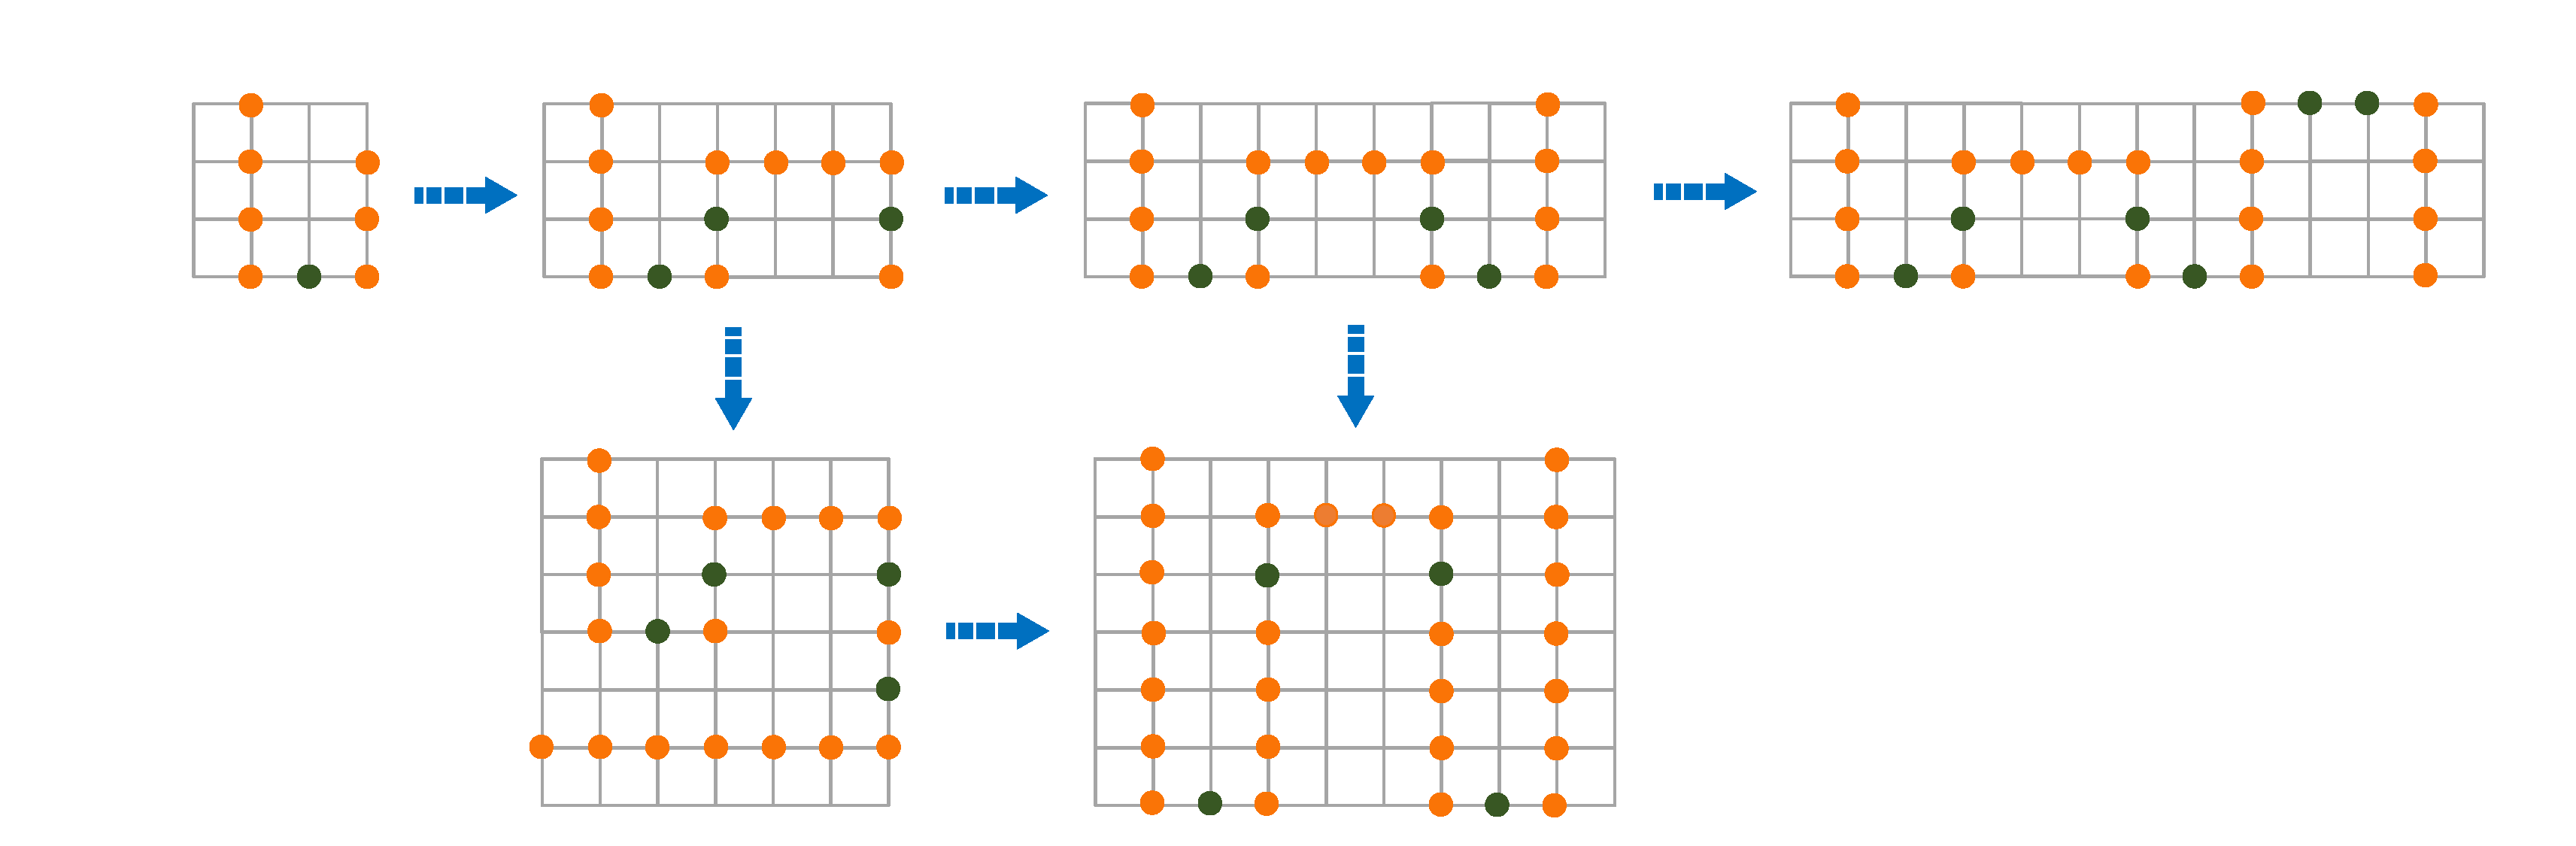
\includegraphics[width=1.0\linewidth]{pix/sensing-traj/path_case_4.pdf}
\caption{Minimum dominating path when $m \equiv 1 \pmod 3$, $n \equiv 1 \pmod 3$.}
\label{fig:path_case_4}
\end{minipage}%
\end{figure}

\vspace{-0.1in}

\subsection{How to concatenate 2D trajectories to a 3D one}
In a real-world 3D space that might be irregular, we give an approach to concatenate 2D trajectories to a 3D trajectory.
\begin{itemize}
  \item First, we divide 3D space into cuboids and obtain a 3D irregular grid; and then we further divide the 3D grid into multiple layers of 2D irregular grids.
  \item Then, for each irregular 2D grid, we could divide it into a number of regular 2D grids. In each regular 2D grid, we can use the proposed algorithm to construct the minimum dominating path for it.
  \item Finally, we could simply concatenate the minimum dominating paths for those regular grids because their end points always lie on the grid boundary, which produce a trajectory for the drone in the 3D space.
\end{itemize}

%\begin{algorithm}[htb]
%\caption{Trajectory planning for UAV in grid when consider total time consuming}
%\label{alg:Framwork2}
%\begin{algorithmic}[1]
%\Require
%The graph of trajectory planning, $L_{m,n}$;
%The length of grid, $m$;
%The width of gird, $n$;
%\Ensure
%The trajectory of two-dimensional coordinate of grid, $V_P$;
%The COL set of two-dimensional coordinate of grid, $V_C$;
%\label{code:fram:judgemod}
%\State do algorithm 1 and get $V_P$.
%
%\label{code:fram:calculateab}
%\State $a=\lfloor \frac{m}{3} \rfloor$, $b=\lfloor \frac{m}{3} \rfloor$, $ra \equiv m \pmod 3$, $rb \equiv n \pmod 3$;
%
%\label{code:fram:calculate}
%\If{$m<4$ or $n<4$}
%    \If{$(m=1$ and $n \leq 3)$ or $m \geq 2$}
%        \State $V_C=V_P$;
%%        \If{$n<3$}
%%            \State $V_C=V_P$;
%%        \Else
%%            \For{$i=0$ to $b-1$}
%%                \State put $v_{1, 3i+2}$ into $V_C$;
%%            \If{$n \equiv 1 \pmod 3$ or $n \equiv 2 \pmod 3$}
%%                \State put $v_{1, 3b+1}$ into $V_C$;
%%            \EndIf
%%            \EndFor
%%        \EndIf
%
%    \Else
%        \State put $v_{1,2}$, $v_{1,5}$, ..., $v_{1, 3b-1}$ into $V_C$;
%        \State \textbf{If} $rb=1$ or $rb=2$, \textbf{then} put $v_{1,3b+1}$ into $V_C$
%    \EndIf
%
%\ElsIf{$m \equiv 0 \pmod 3$}
%    \State put $G^r_2$, $G^r_5$ ... , $G^r_{3a-1}$ into $V_C$;
%
%%    \For{$i=1$ to $n$}
%%        \For{$j=0$ to $a-1$}
%%            \State put $v_{3*j+2, i}$ into $V_C$;
%%        \EndFor
%%    \EndFor
%
%\ElsIf{$m \equiv 2 \pmod 3$}
%    \If{$a>2$}
%        \State put $v_{2,1}$, $v_{3,1}$, $v_{6,2}$, $v_{7,2}$ into $V_C$;
%
%        \State put $G^r_2$, $G^r_5$ except0 vertices in $G^c_1$ into $V_C$;
%
%        \State put $G^r_8$ except vertices in $G^c_1$ and $G^c_3$ into $V_C$;
%
%        \State put $G^r_10$, $G^r_13$..., $G^r_{3a+1}$ into $V_C$;
%
%%        \For{$i=2$ to $n$}
%%            \State put $v_{2,i}$, $v_{5,i}$, $v_{8,i}$ into $V_C$;
%%        \EndFor
%%
%%        \For{$i=1$ to $n$}
%%            \For{$j=3$ to $a$}
%%                \State put $v_{3*j+1, i}$ into $V_C$;
%%            \EndFor
%%        \EndFor
%
%    \Else
%        \State put $G^r_2$ into $V_C$;
%        \State put $G^r_4$, ..., $G^r_{3a+1}$ into $V_C$;
%
%%        \For{$i=1$ to $n$}
%%            \State put $v_{2,i}$ into $V_C$;
%%        \EndFor
%%
%%        \For{$i=1$ to $n$}
%%            \For{$j=1$ to $a$}
%%                \State put $v_{3*j+1, i}$ into $V_C$;
%%            \EndFor
%%        \EndFor
%    \EndIf
%
%\Else
%
%    \If{$a \leq 2$ and $b \leq 2$}
%        \State \textbf{if} $a \geq 1$ and $b \geq 1$, \textbf{then} put $v_{1,2}$, $v_{2,2}$, $v_{3,2}$, $v_{4,2}$, $v_{4,4}$, $v_{3,4}$, $v_{2,4}$ into $V_C$;
%
%        \State \textbf{if} $a \geq 1$ and $b=2$, \textbf{then} put $v_{2,5}$, $v_{2,6}$, $v_{2,7}$, $v_{4,7}$ into $V_C$ and move $v_{3,4}$ out from $V_C$;
%
%        \State \textbf{if} $a=2$, \textbf{then} put $v_{6,7}$, $v_{6,6}$, $v_{6,5}$, $v_{6,4}$, $v_{6,3}$, $v_{6,2}$, $v_{6,1}$ into $V_C$;
%
%%    \If{$a=1$ and $b=1$}
%%        \State put $v_{1,2}$, $v_{2,2}$, $v_{3,2}$, $v_{4,2}$, $v_{4,4}$, $v_{3,4}$, $v_{2,4}$ into $V_C$;
%%
%%    \ElsIf{$a=1$ and $b=2$}
%%        \State put $v_{1,2}$, $v_{2,2}$, $v_{3,2}$, $v_{4,2}$, $v_{4,4}$, $v_{2,4}$, $v_{2,5}$, $v_{2,6}$, $v_{2,7}$, $v_{4,7}$ into $V_C$;
%%
%%    \ElsIf{$a=2$ and $b=2$}
%%        \State put $v_{1,2}$, $v_{2,2}$, $v_{3,2}$, $v_{4,2}$, $v_{4,4}$, $v_{2,4}$, $v_{2,5}$, $v_{2,6}$, $v_{2,7}$, $v_{4,7}$, $v_{6,7}$, $v_{6,6}$, $v_{6,5}$, $v_{6,4}$, $v_{6,3}$, $v_{6,2}$, $v_{6,1}$ into $V_C$;
%
%    \Else
%        \State put $v_{2,4}$, $v_{2,5}$, $v_{2,6}$, $v_{2,7}$ into $V_C$;
%
%        \State put $G^c_2$ into $V_C$;
%
%        \State put $G^c_4$, $G^c_7$ except for $G^r_{1,3}$ into $V_C$;
%
%        \State put $G^c_{10}$, $G^c_{13}$, ..., $G^c_{3b}$ into $V_C$;
%
%%        \For{$i=1$ to $m$}
%%            \State put $v_{i,2}$ into $V_C$;
%%        \EndFor
%%
%%        \For{$i=4$ to $m$}
%%            \State put $v_{i,4}$, $v_{i,7}$ into $V_C$;
%%        \EndFor
%%
%%        \For{$i=1$ to $m$}
%%            \For{$j=3$ to $b$}
%%                \State put $v_{i, 3*j}$ into $V_C$;
%%            \EndFor
%%        \EndFor
%    \EndIf
%\EndIf
%
%\Return $V_P$, $V_C$;
%\end{algorithmic}
%\end{algorithm}

%From last subsection, we know how to find the minimum dominating path in $L_{m,n}$. Therefore, we just have to find the set of COLs $V_C$ in dominating path $L$. However, since we have already discussed dominating vertices in last subsection, we only need to add all dominating vertices into $V_C$. In general, we only have 1 case for COL which is $standard extend row$ and in this case, we just take the entire row into $V_C$ and add
%
%Therefore, for the 6 different cases, we have the following result.
%
%\begin{prop}
%$\\$
%\begin{enumerate}
%  \item $\gamma_l(L_{1,n})=\lfloor \frac{n+2}{3} \rfloor$
%  \item $\gamma_l(L_{2,2})=\gamma_l(L_{2,3})=2$, and if $4 \leq n$, $\gamma_l(L_{2,n})=n$
%  \item $\gamma_l(L_{3,n})=n$
%\end{enumerate}
%\end{prop}
%
%\begin{prop}
%Assume $m \geq 4$, $n \geq 4$. When $m \equiv 0 \pmod 3$, $n \equiv 1 \pmod 3$, we have $|V_C|=3ab+a$. When $m \equiv 2 \pmod 3$, $n \equiv 1 \pmod 3$, we have
%\[
%\begin{aligned}
%&|V_C|\\
%&=\left\{
%\begin{array}{rcl}
%3ab+a+3b+1       &      & {a \leq 2}\\
%3ab+a+3b+2       &      & {otherwise}\\
%\end{array} \right.
%\end{aligned}
%\].
%\end{prop}
%
%% TODO »¯Œò b СÓÚµÈÓÚ 2 µÄÇé¿ö£¬ÔöŒÓ 1¡¢2¡¢3µÄÇé¿ö
%\begin{prop}
%Assume $m \geq 4$, $n \geq 4$. When $m \equiv 0 \pmod 3$, $n \equiv 0 \pmod 3$, we have
%$|V_C|=3ab$.
%When $m \equiv 0 \pmod 3$, $n \equiv 2 \pmod 3$, we have
%\[
%\begin{aligned}
%&|V_C|\\
%&=\left\{
%\begin{array}{rcl}
%3ab+2a       &      & {b \leq 2, 3ab+4a-2 \leq 3ab+3a+2b-1}\\
%3ab+3a       &      & {b \leq 2, 3ab+4a-2 > 3ab+3a+2b-1}\\
%3ab+2a       &      & {b > 2, 3ab+4a-2 \leq 3ab+3a+2b-2}\\
%3ab+3a+1       &      & {otherwise}\\
%\end{array} \right.
%\end{aligned}
%\].
%When $m \equiv 2 \pmod 3$, $n \equiv 2 \pmod 3$, assume $m \leq n$, we have
%\[
%\begin{aligned}
%&|V_C|\\
%&=\left\{
%\begin{array}{rcl}
%3ab+2a+3b+2       &      & {a \leq 2}\\
%3ab+2a+3b+3       &      & {otherwise}\\
%\end{array} \right.
%\end{aligned}
%\].
%Besides, the results have a same structure.
%\end{prop}
%
%\begin{prop}
%Assume $m \geq 4$, $n \geq 4$. When $m \equiv 1\pmod 3$, $n \equiv 1\pmod 3$, $a \geq 1$ and $b \geq 1$, assume $m \leq n$, we have
%\[
%\begin{aligned}
%&|V_C|\\
%&=\left\{
%\begin{array}{rcl}
%7        &      & {a=1, b=1}\\
%10       &      & {a=1, b=2}\\
%17       &      & {a=2, b=2}\\
%3ab+3a+b-1       &      & {otherwise}\\
%\end{array} \right.
%\end{aligned}
%\].
%\end{prop}

% Ïà¹ØËã·š



\section{Evaluation}\label{sec:experiment}

% ·ÂÕæ
% ʵÑé׌±ž£¬¿ÉÒÔÄ£·Â mobicom ÄÇƪµÄÐŽ·š£¬°ÑһЩӲŒþҲЎœøÈ¥£¬AQI Ö»ÊÇžöžºÖصÄÀý×Ó£¬Ä¿µÄÊÇÎÒÃÇÕâžöÊÇ general 3D sensing ¶Œ¿ÉÒÔÓ㬲»Ò»¶šÖ»ÊDzâÁ¿ AQI¡£
% ÕæʵµÄ·Å·ÉʵÑ飬¿Ž¿Žµç³ØÄܷɶàŸÃ¡£
\begin{figure}
\centering
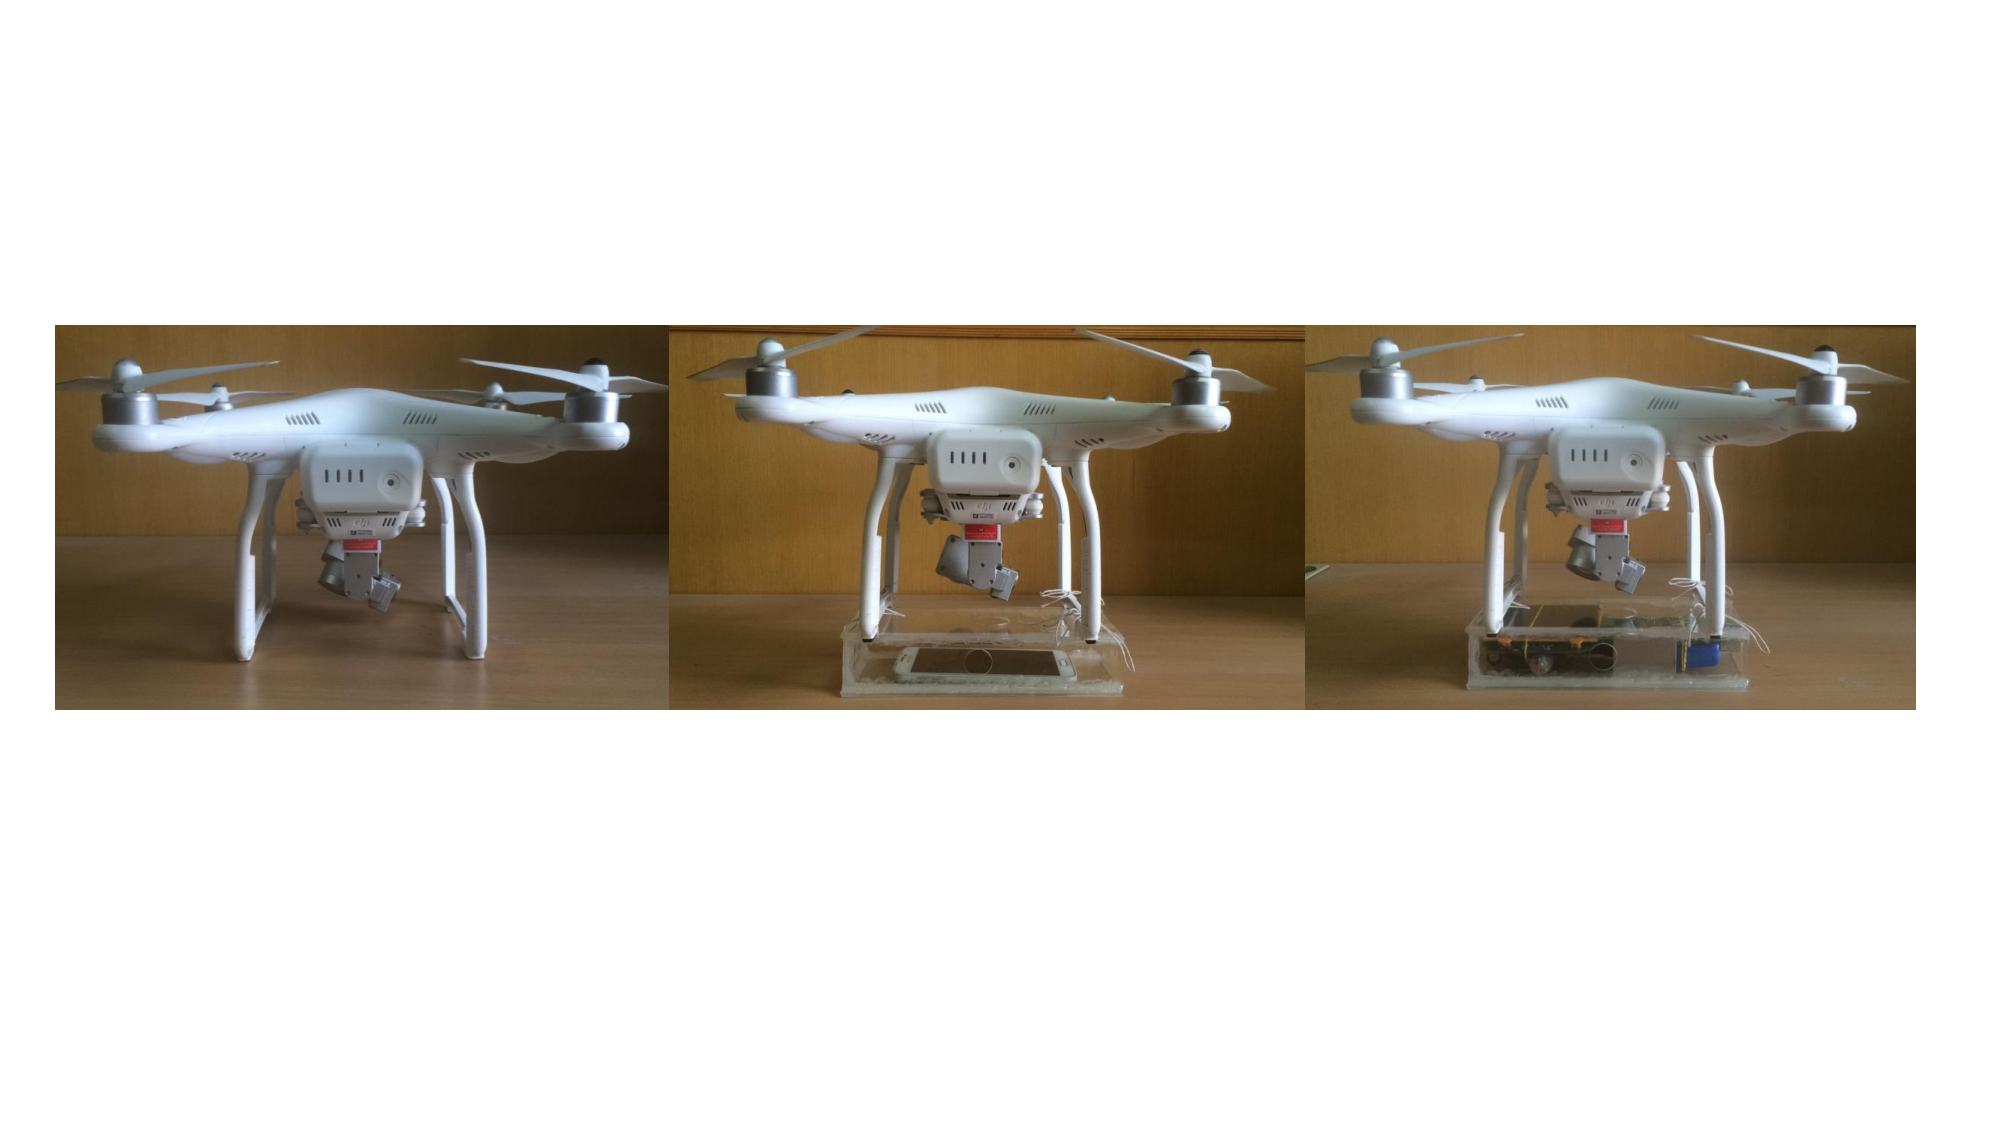
\includegraphics[width=0.8\linewidth]{pix/sensing-traj/eva_uav.pdf}
\caption{DJI Phantom 3 quadcopter.}
\vspace{-0.15in}
\label{fig:eva_uav}
\end{figure}

\begin{figure*}
\begin{minipage}[c]{0.23\textwidth}
\centering
% time  fig:time
% coverage
% time-load
% coverage-load
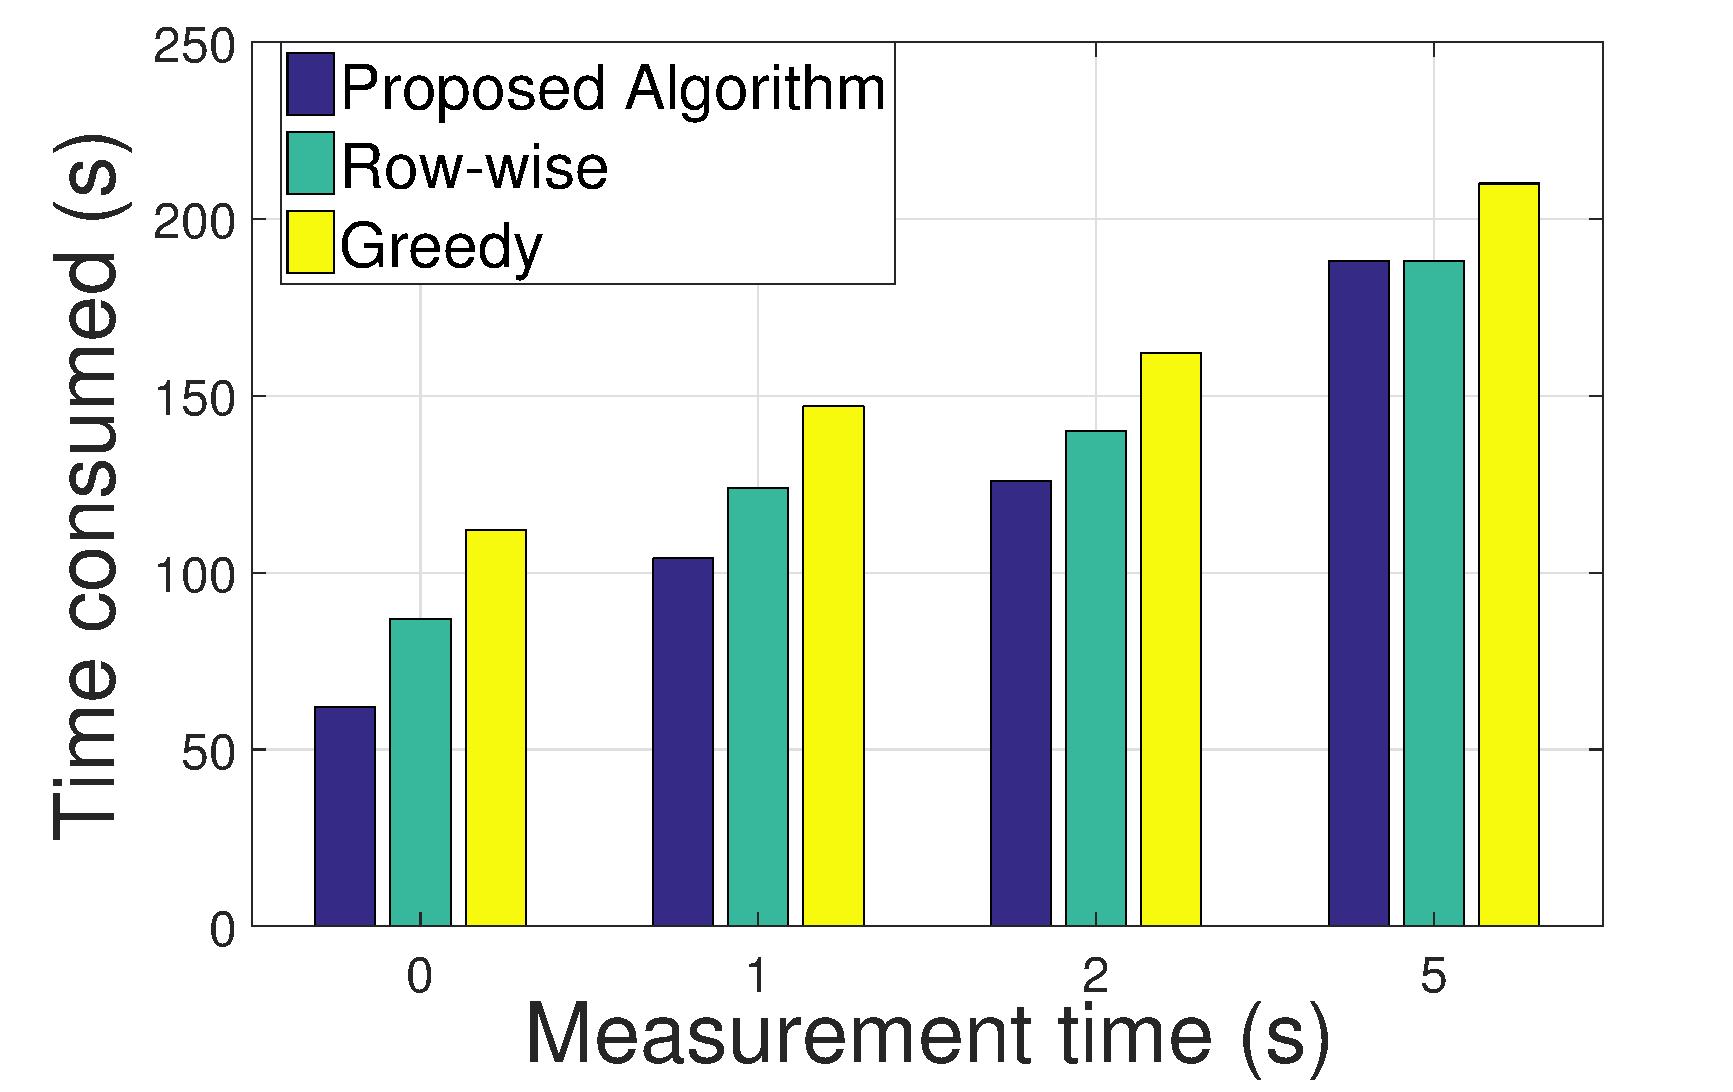
\includegraphics[width=1.0\linewidth]{pix/sensing-traj/eva_time.pdf}
\caption{Time consumed of three algorithms with different granularity of measurement time.}
\label{fig:eva_time}
\end{minipage}%
\hfill
\begin{minipage}[c]{0.23\textwidth}
\centering
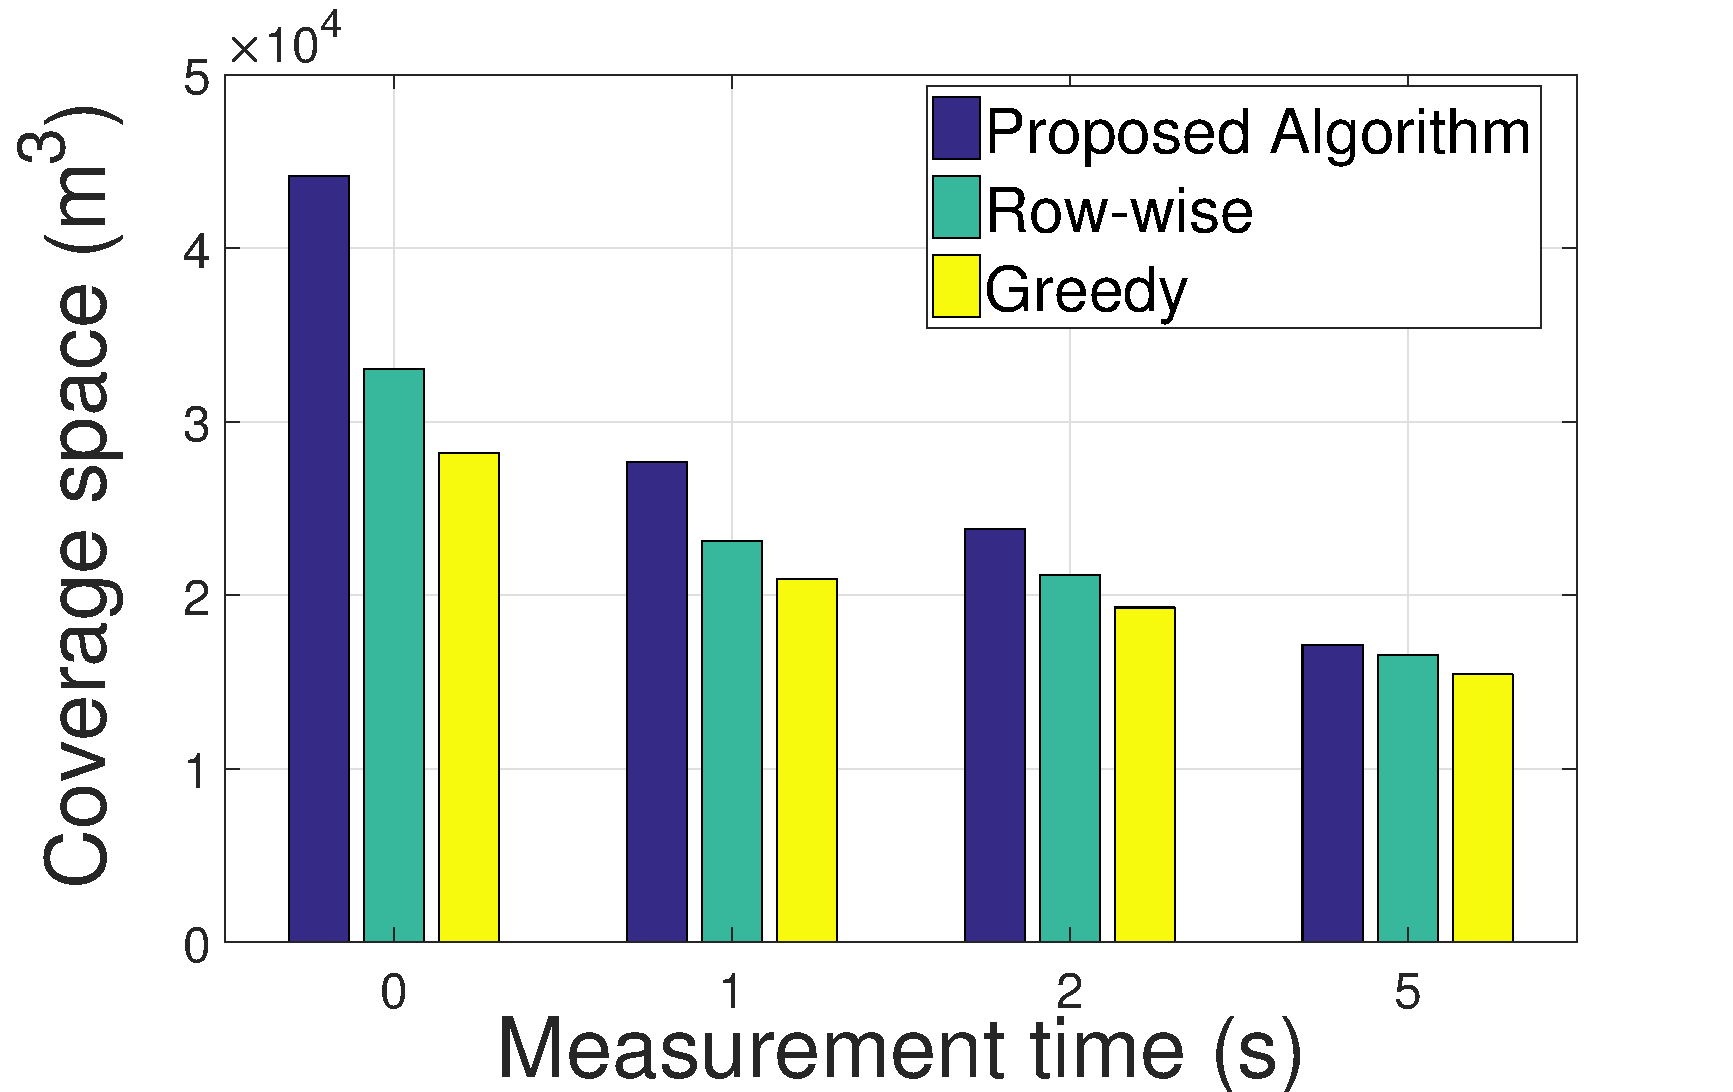
\includegraphics[width=1.0\linewidth]{pix/sensing-traj/eva_coverage.pdf}
\caption{Coverage space of three algorithms with different granularity of measurement time.}
\label{fig:eva_coverage}
\end{minipage}
\hfill
\begin{minipage}[c]{0.23\textwidth}
\centering
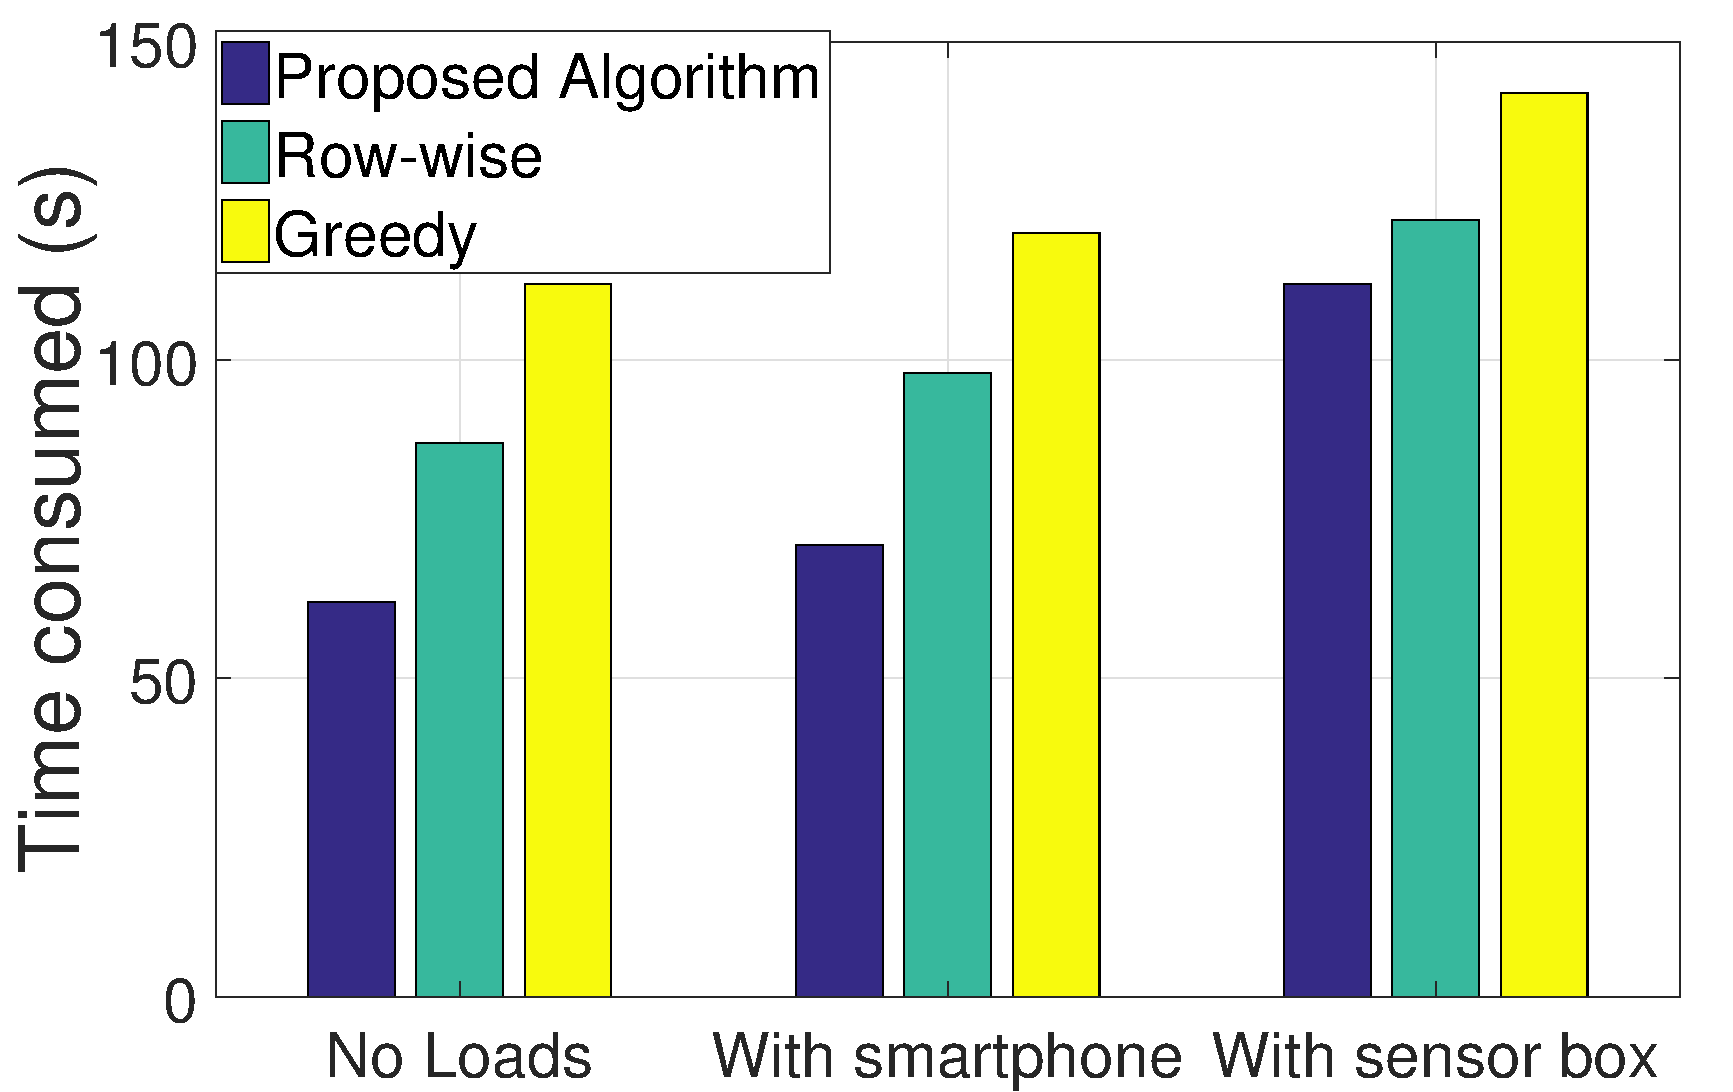
\includegraphics[width=1.0\linewidth]{pix/sensing-traj/eva_time_load.pdf}
\caption{Time consumed of three algorithms with different loads.}
\label{fig:eva_time_load}
\end{minipage}
\hfill
\begin{minipage}[c]{0.23\textwidth}
\centering
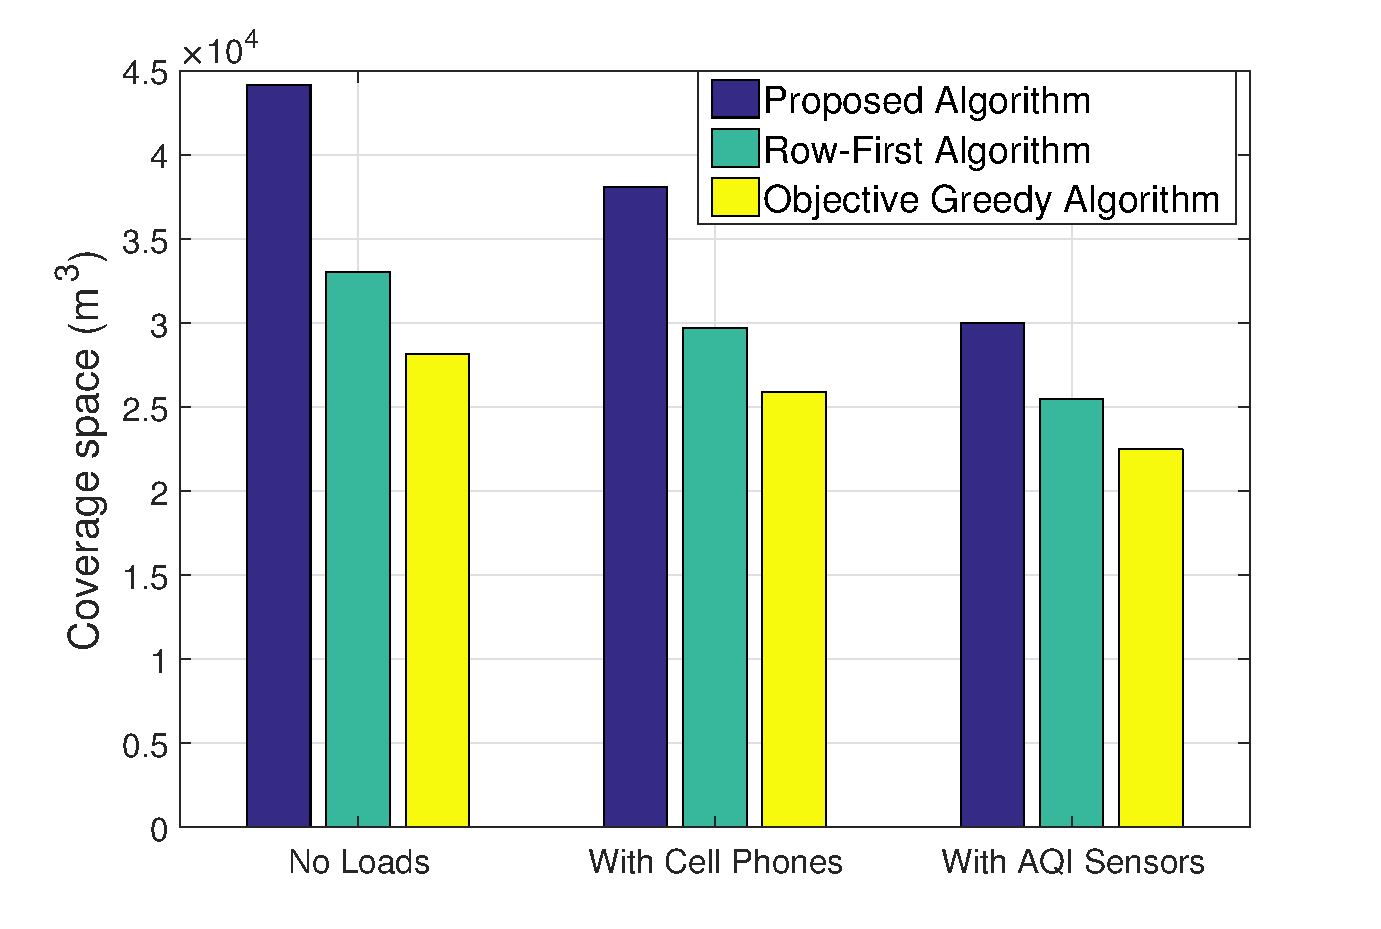
\includegraphics[width=1.0\linewidth]{pix/sensing-traj/eva_coverage_load.pdf}
\caption{Coverage space of three algorithms with different loads.}
\label{fig:eva_coverage_load}
\end{minipage}
\end{figure*}
%XXX w/ smartphones; w/ sensor box



%\begin{figure*}
%\begin{minipage}[t]{0.3\textwidth}
%\centering
%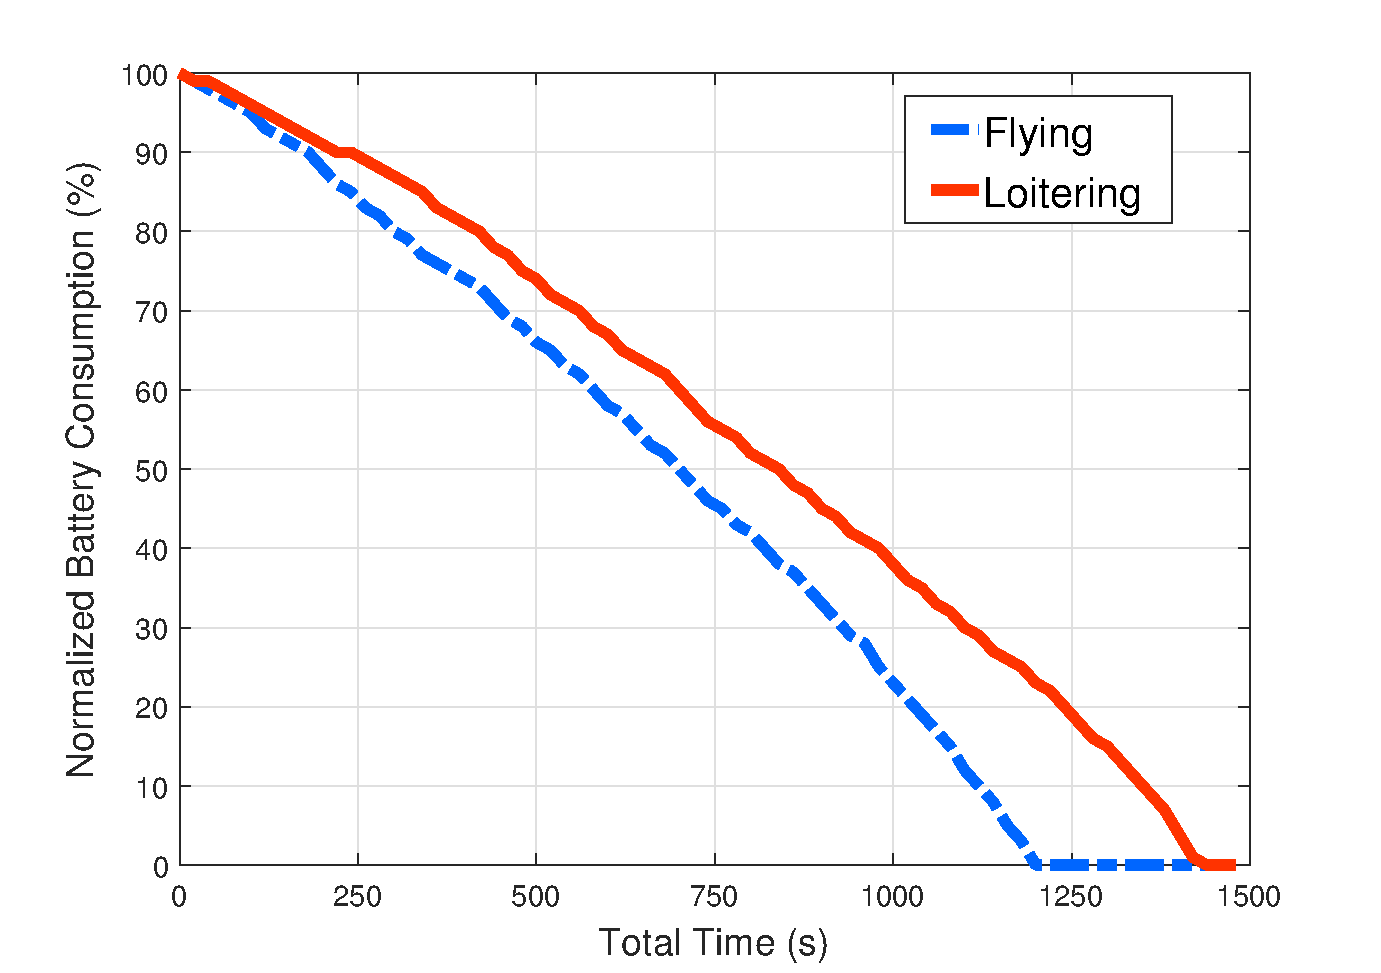
\includegraphics[width=0.8\linewidth]{pix/sensing-traj/eva_time_battery.pdf}
%\caption{Comparison of the Adaptive Monitoring Algorithm, Greedy Algorithm and Sequential Selection.}
%\label{fig:eva_time_battery}
%\end{minipage}%
%\hfill
%\begin{minipage}[t]{0.3\textwidth}
%\centering
%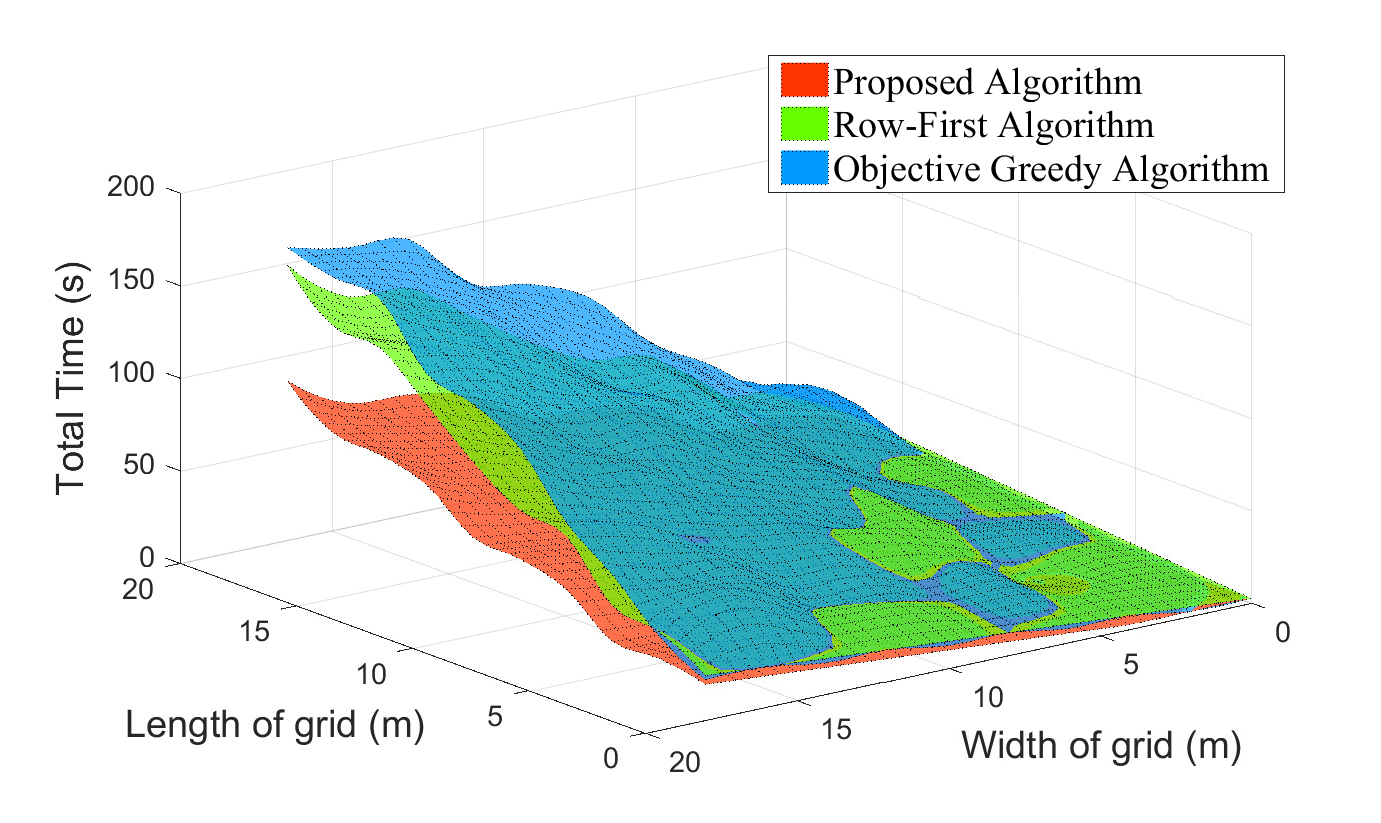
\includegraphics[width=0.8\linewidth]{pix/sensing-traj/eva_grid_time.pdf}
%\caption{Comparison of the Adaptive Monitoring Algorithm, Greedy Algorithm and Sequential Selection.}
%\label{fig:eva_grid_time}
%\end{minipage}
%\hfill
%%\begin{minipage}[t]{0.3\textwidth}
%%\centering
%%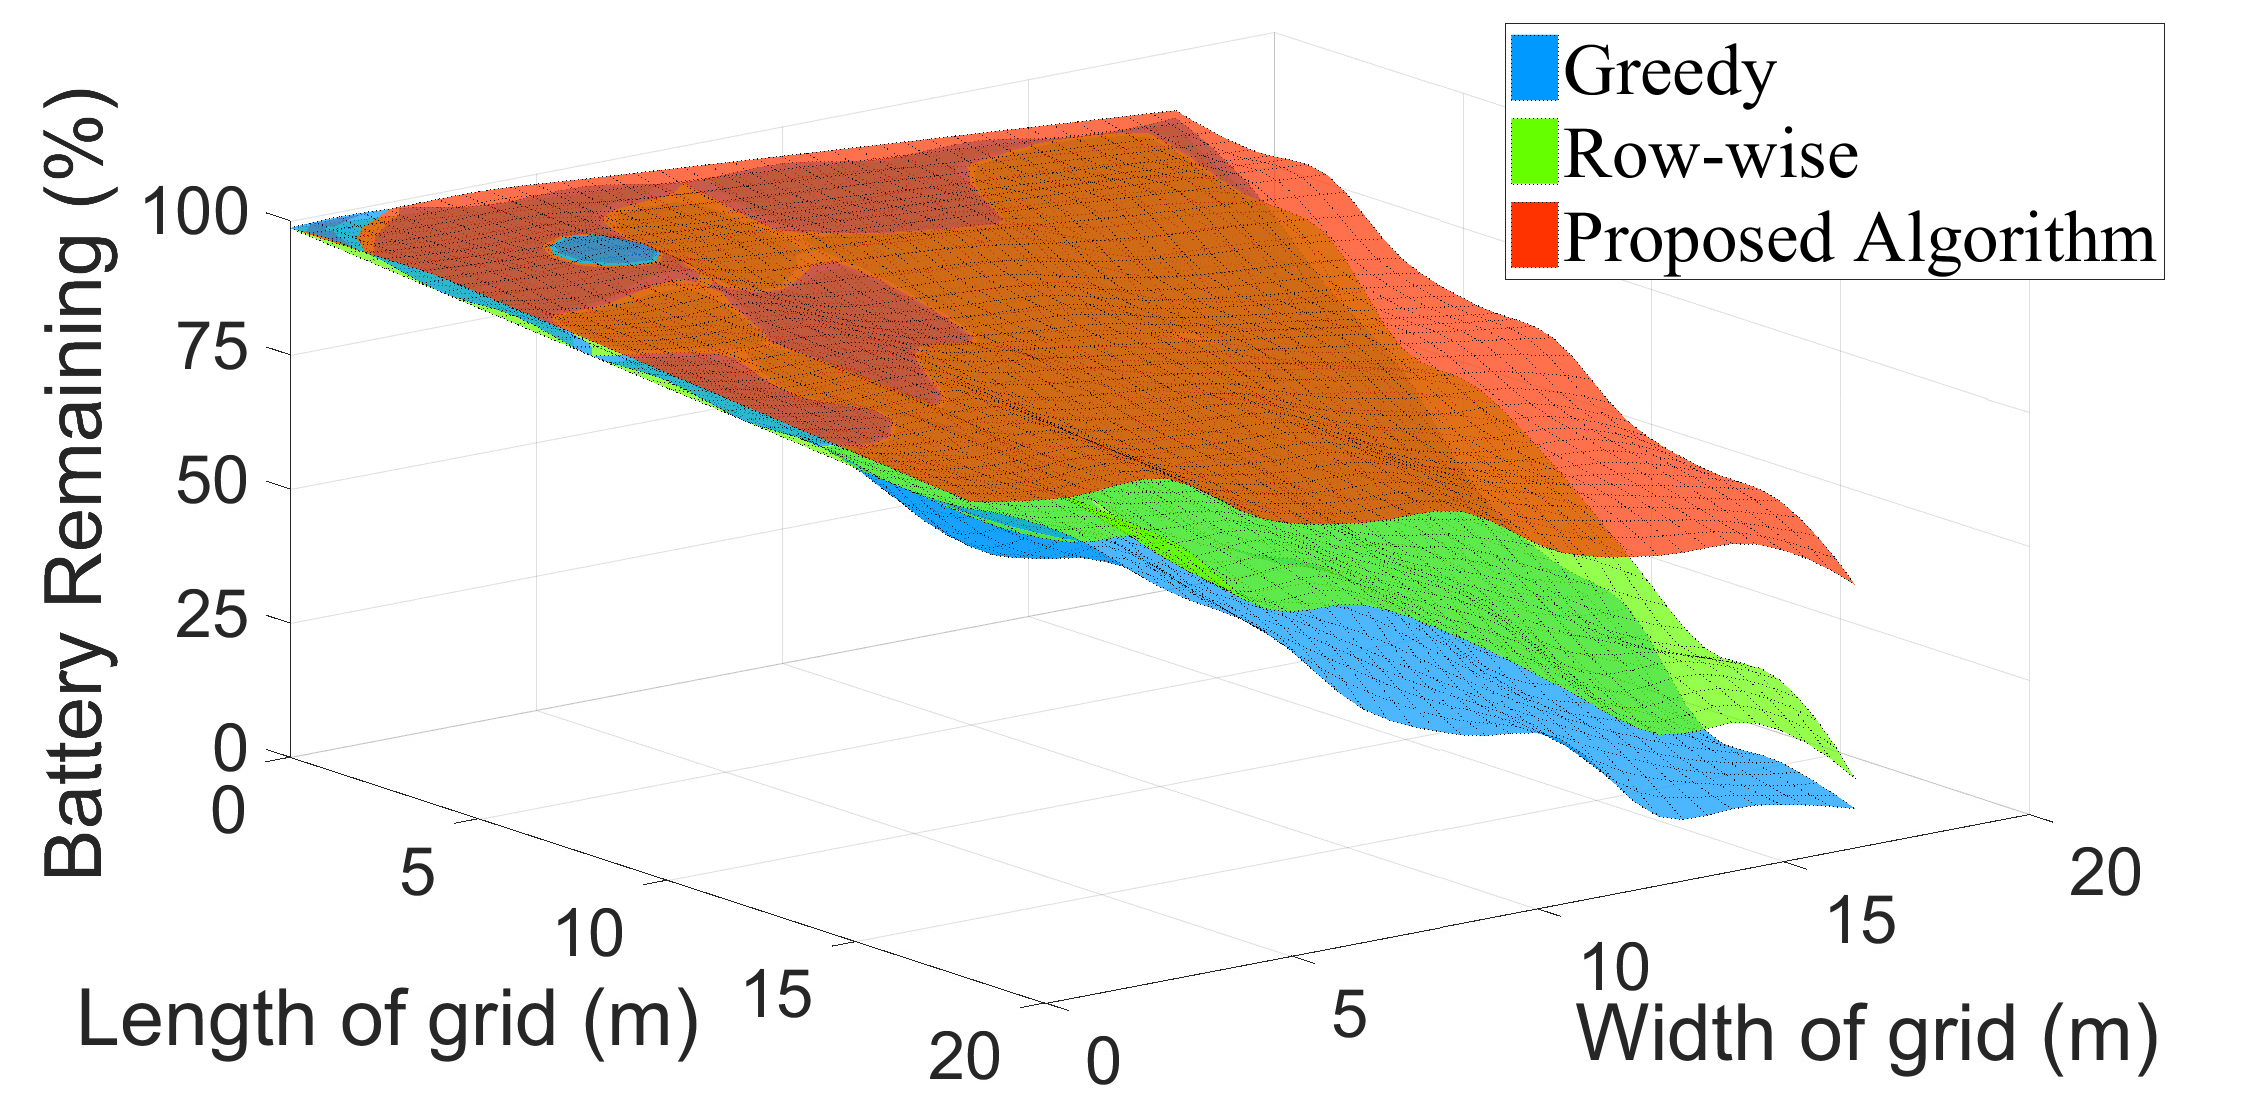
\includegraphics[width=0.8\linewidth]{pix/sensing-traj/eva_grid_battery.pdf}
%%\caption{Comparison of the Adaptive Monitoring Algorithm, Greedy Algorithm and Sequential Selection.}
%%\label{fig:eva_grid_battery}
%%\end{minipage}
%\end{figure*}

%\begin{figure*}
%\centering
% \begin{subfigure}[b]{0.23\linewidth}
%    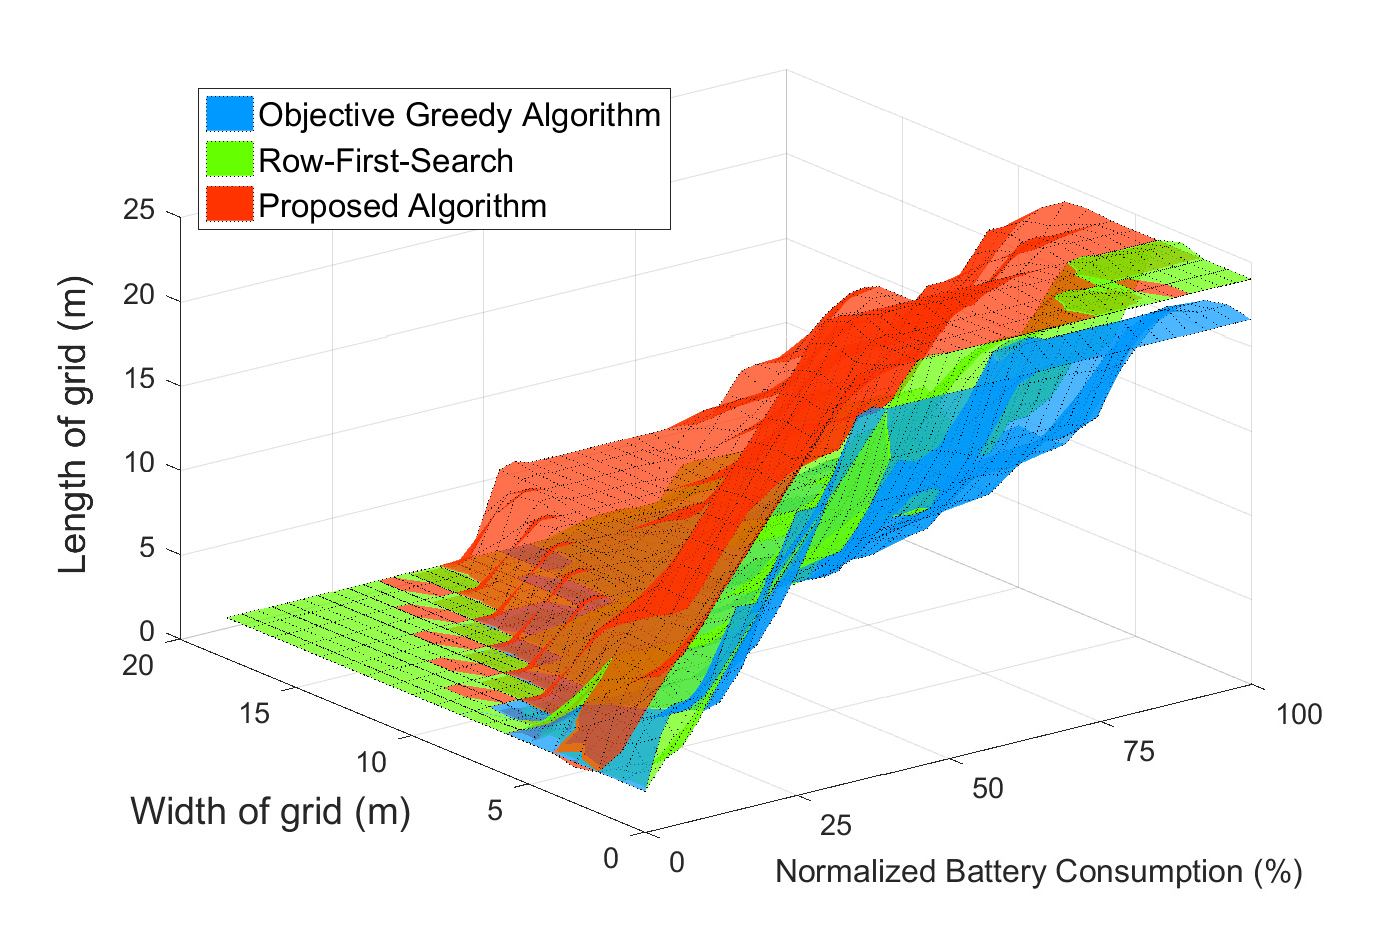
\includegraphics[width=1.0\linewidth]{pix/sensing-traj/eva_battery.pdf}
%    \caption{Based on Message Diffusion.\\~}
%    \label{fig:FPIM:a}
%\end{subfigure}
% \begin{subfigure}[b]{0.23\linewidth}
%    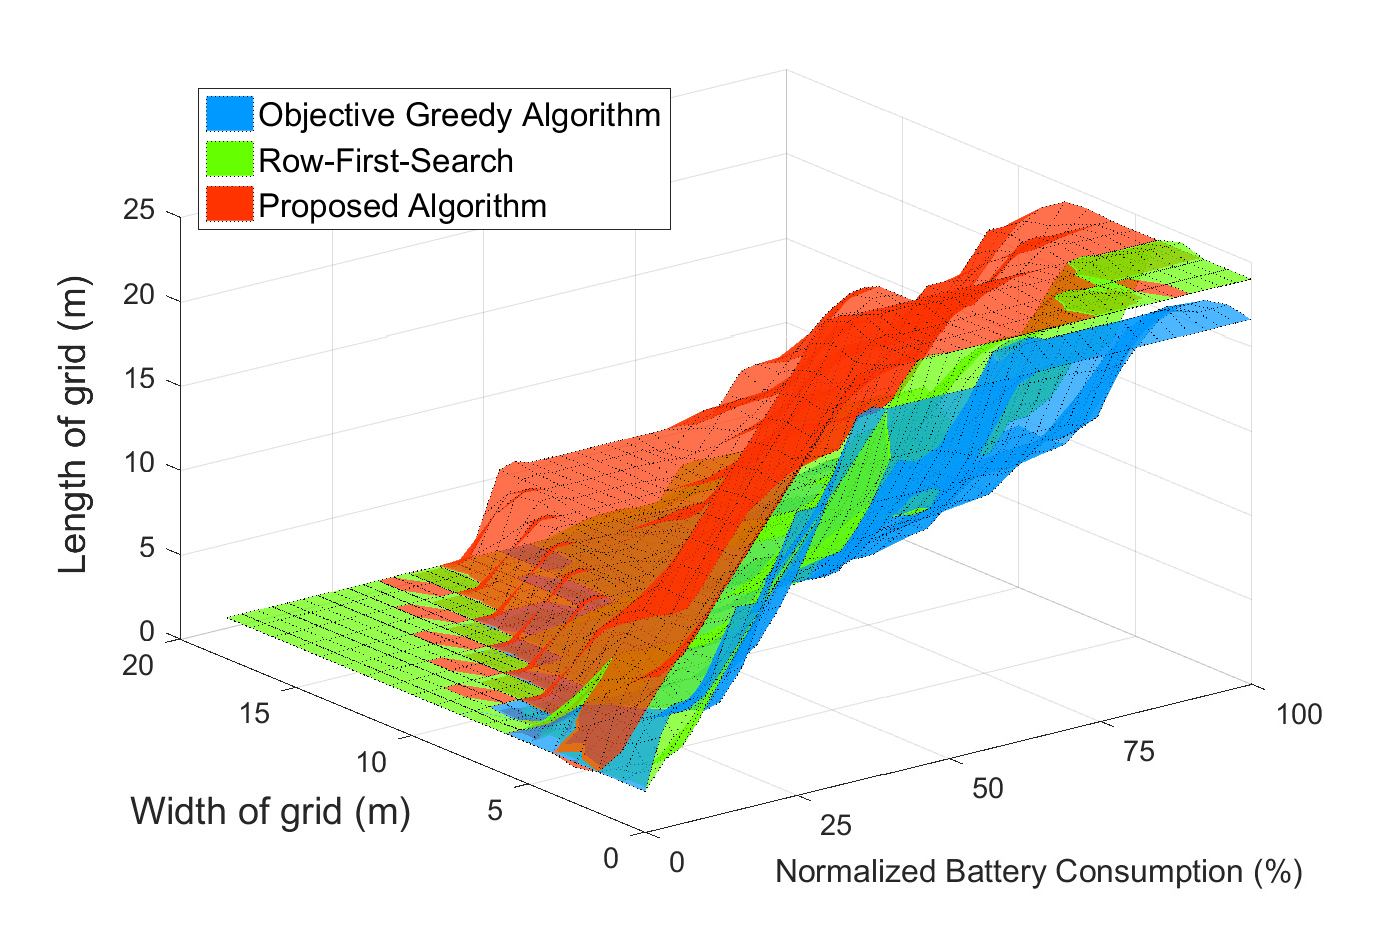
\includegraphics[width=1.0\linewidth]{pix/sensing-traj/eva_battery.pdf}
%    \caption{Based on $P_\mathbb{S}$.\\~}
%    \label{fig:FPIM:b}
%\end{subfigure}
% \begin{subfigure}[b]{0.23\linewidth}
%    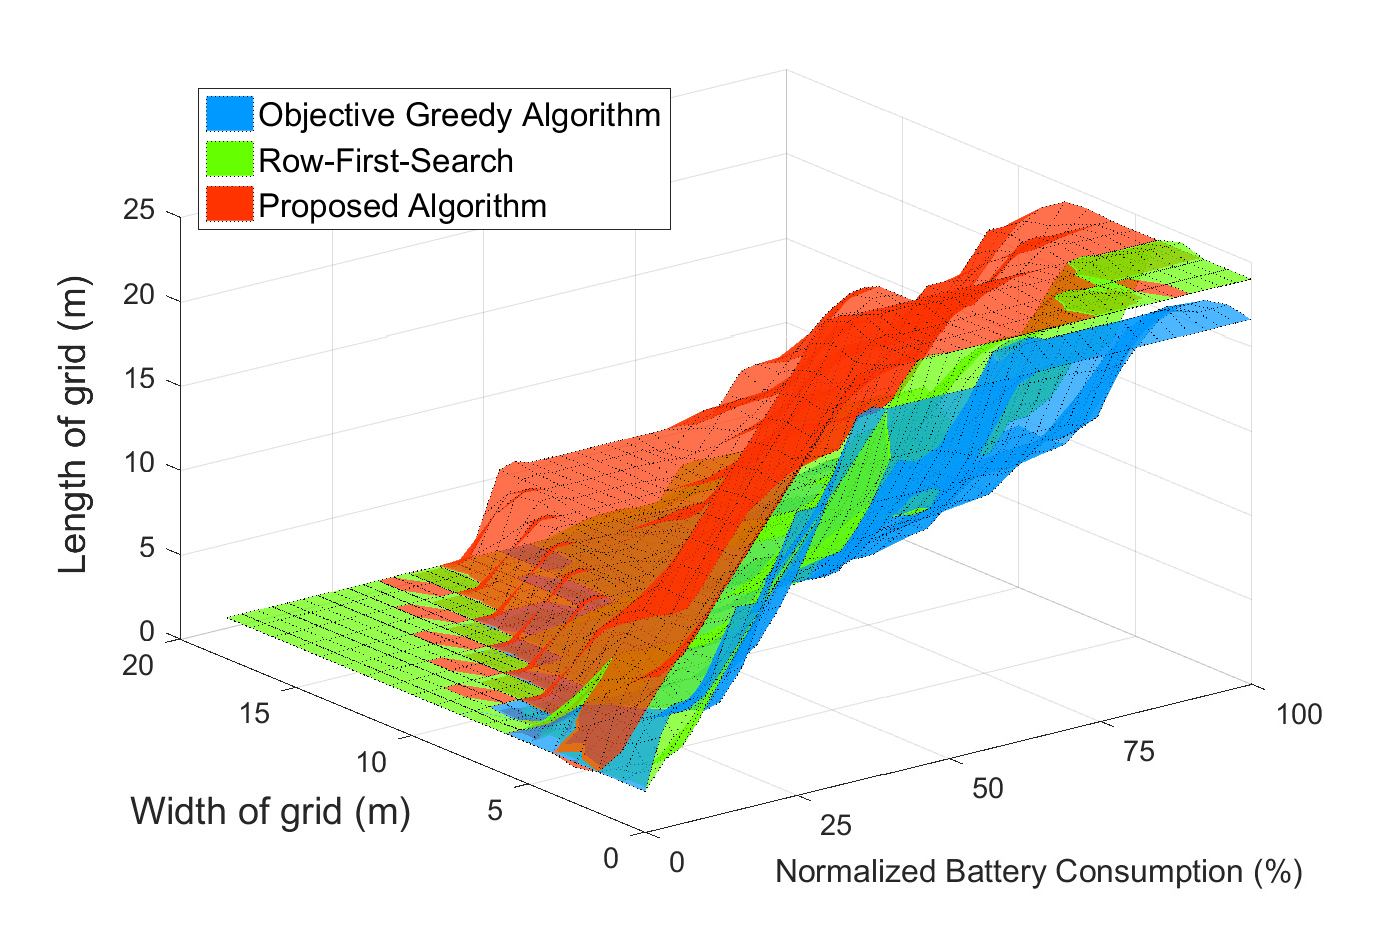
\includegraphics[width=1.0\linewidth]{pix/sensing-traj/eva_battery.pdf}
%    \caption{Based on $P_{\Delta\mathbb{S}}$.\\~}
%    \label{fig:FPIM:c}
%\end{subfigure}
% \begin{subfigure}[b]{0.23\linewidth}
%    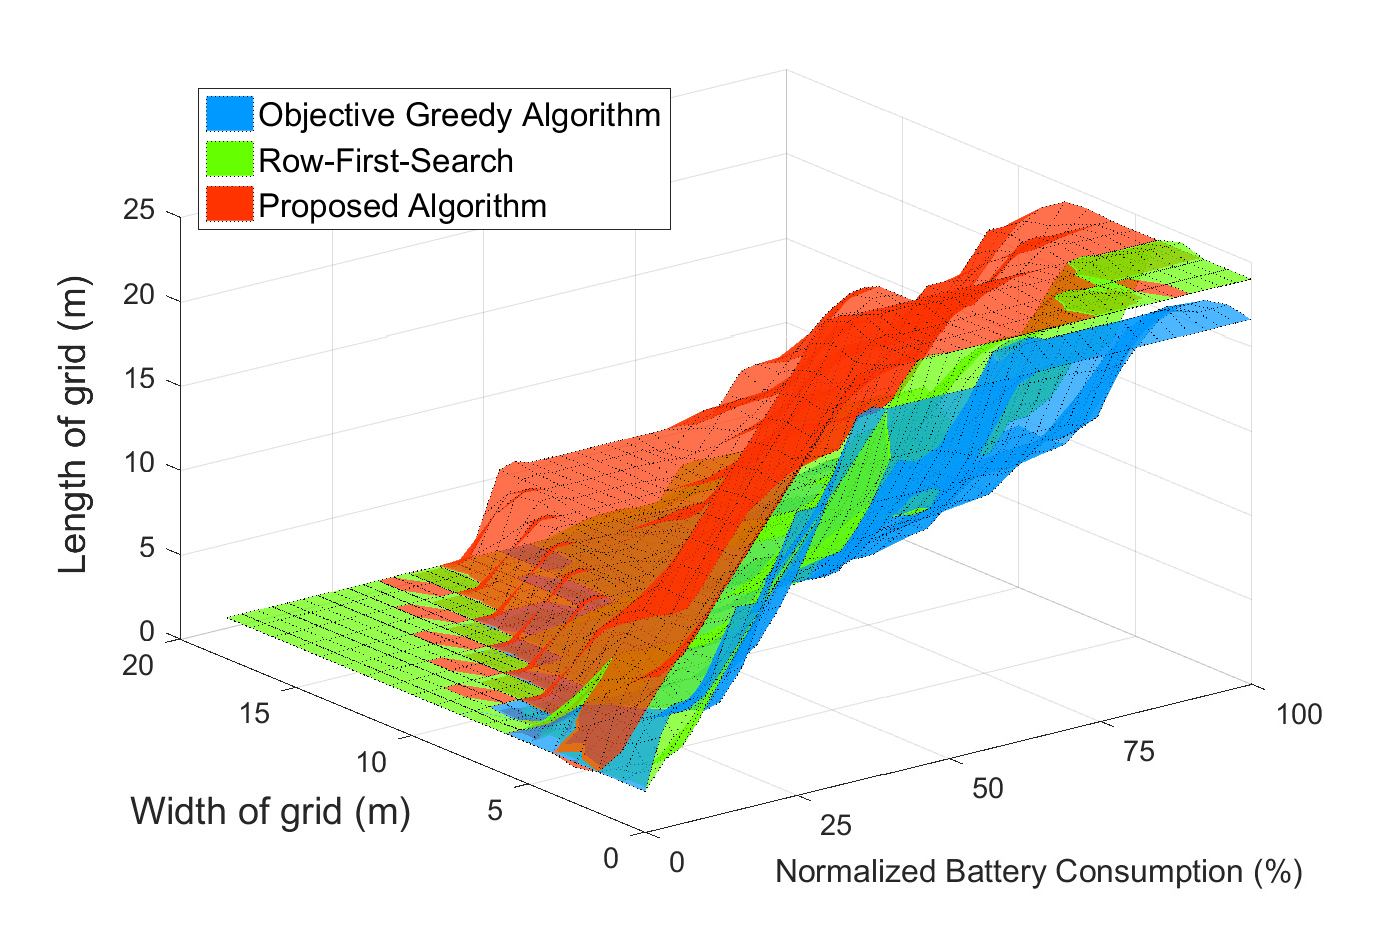
\includegraphics[width=1.0\linewidth]{pix/sensing-traj/eva_battery.pdf}
%    \caption{Proportion of correct predictions.}
%    \label{fig:FPIM:d}
%\end{subfigure}
%\caption{Results of inferring the floating population (FP) that has excluded those whose home and remote regions are the same.}
%\label{fig:FPIM}
%\end{figure*}


\subsection{Experiment Setup}


\textbf{Prototype}:
The prototype consists of two parts: (1) a drone with an API that can configure its trajectory; and (2) a measurement sensor board or a smartphone is installed into a plastic box with vent-holes made by a laser engraving machine, which is attached at the bottom of the drone. The drone we use is a DJI Phantom 3 quadcopter, as shown in Figure~\ref{fig:eva_uav}. There is an intelligent flight mode that allows the customization of the trajectory by configuring a number of stop locations such that the drone will autonomously follow this trajectory to hover over each stop and complete the flight. The GPS sensor, ultrasonic sensor, and the motion sensors collectively determine the current observation location of the drone and guide the drone to the next stop in the trajectory. At each stop, the drone hover for a few seconds, $t_M$, to collect sufficient measurement data, before traversing to the next stop.


% We use drones to verify our results. Since we divide 3D space into OL-network by cuboids which forms a 3D grid partitioned by height, we only consider algorithms in 2D grid.

\textbf{Compared algorithms}: We compare the proposed algorithm with two other conventional algorithms. In the proposed algorithm, we choose the minimum dominating path in grids first, and then select COLs from path. In contrast, the conventional algorithms we considered will select COLs in grids first, and then choose a path to connect the selected COLs. The two conventional algorithms differ by the way of selecting COLs, as introduced below.
\begin{enumerate}
  \item \emph{Row-wise COL selection}: We select the minimum dominating set in grids first~\cite{alanko2011computing,gonccalves2011domination,chang1992domination}, and select an OL at boundary as start point. Then, we use a row-first COL selection strategy to find a row by row, along the longer side of the grid.
  \item \emph{Greedy COL selection}: We select the minimum dominating set in grids first, and then select a COL at boundary as start point. Then, we follow the greedy algorithm that chooses the next vertex $v$ as the closest one that can lead to the maximum coverage, such as:
      $       \min\limits_{d(v,v')} \max\limits_{ |N[v]\setminus N[P]| } v,       $
      where $v' \in \mathcal{G}$ is the last vertex of path of $P \subset \mathcal{G}$.
\end{enumerate}

\textbf{Performance metrics}: We use the following two metrics for evaluating the algorithm performance.
\begin{itemize}
  \item \emph{Time consumed}: The time consumed is defined as total time of flight and measurement of the drone to cover the space of the trajectory under a specific algorithm.
  \item \emph{Coverage space}: The coverage space is defined as the maximum coverage area in the 3D space during entire battery life, by following the trajectory under a specific algorithm. %  Since algorithm is affected by input width and length, We fix the width of grid.
\end{itemize}

\subsection{Experimental Results}
We choose an open space in a university campus which has a size of 45~m in length, 35~m in width, and 10~m in height. It is divided into 3D grids formed by 5 by 5 by 5~m cuboids. Since the time consumed is the sum of flight time and measurement time, we consider the impact of different measurement times in experiments, which are set as 0, 1, 2, 5 seconds at each COL. 

\textbf{Time consumed}:
Figure~\ref{fig:eva_time} show the time consumed under compared algorithms with different granularity of the measurement time. The sensing area is a 2D grid of size 45 by 35~m. We observe that our proposed algorithm consumes less time when the measurement time is small. The gap between our algorithm and the row-wise COL selection algorithm decreases as the measurement time increases. When the measurement time is 5 seconds at each COL, the total time consumed by the proposed and the row-wise COL selection algorithms are equal.

\textbf{Coverage space}:
Figure~\ref{fig:eva_coverage} show the coverage space in the 3D grid under compared algorithms with different granularity of the measurement time during the battery life.
We fix the width of the grid as 30~m, we observe that our proposed algorithm could cover more space than other algorithms in all cases, during the whole battery life. As the measurement time increases, the coverage area by any of three algorithms decreases, since the measurement time consumes part of the battery. Meanwhile, the difference in the coverage space among three algorithms decreases when the measurement time is set greater.

\textbf{Time consumed and the coverage space with different loads}:
In a real-world application, drones might be used to delivery packages or other goods. Hence, we also evaluate the time consumed and the coverage space with different loads when we only consider the flight time. Results in Figure~\ref{fig:eva_time_load} and~\ref{fig:eva_coverage_load} show that as the load increases, the time consumed of three algorithms to complete the sensing task of a given grid increases; meanwhile, the coverage space of three algorithms during the battery life decreases. Note that the proposed algorithm performs the best in all scenarios under different loads on the drone.

\textbf{Results in different-size spaces}:
In experiments, we only test the performance of compared algorithm in a give 3d space with the fixed size. Next, we evaluate the algorithm performance in different-size spaces. Figure~\ref{fig:eva_grid_time} shows the flight time in spaces with different width and length. We observe that our algorithm consumes less time to complete the sensing task in each grid. When fixing the width (or length), the gap among algorithms increases as the length (or width) increases.

%Similarly, we observe in Figure~\ref{fig:battery}, our proposed algorithm has the maximum  coverage space during the battery life; When fixing the width (or length), our algorithm could cover more space than other compared algorithms.

% XXX~We also observe that, when fixing the width, as length increases, the ratio between our algorithm and the row-wise COL selection algorithm could converge to a periodic result.

\section{Conclusions}\label{sec:conclude}
In this paper, we study the optimal trajectory planning problem for mobile sensing in 3D space, where a drone can cover the sensing scope of the space by using the minimum trajectory. We extend the concept of dominating set in graph theory to define the dominating path, and formulate the problem as finding the minimum dominating path in the
grid to cover the sensing scope in 3D space with the minimum trajectory. By dividing the 3D space into a grid of observation locations, we propose an optimal algorithm that first finds the minimum dominating path (trajectory) for the drone, and then selects the least number of critical OLs within the trajectory to perform measurement. Experimental results show that the proposed algorithm can save 32\% less time than existing approaches to complete sensing the given space; during the battery life, it can cover 19\% more sensing scope than existing solutions.

\begin{figure}
\centering
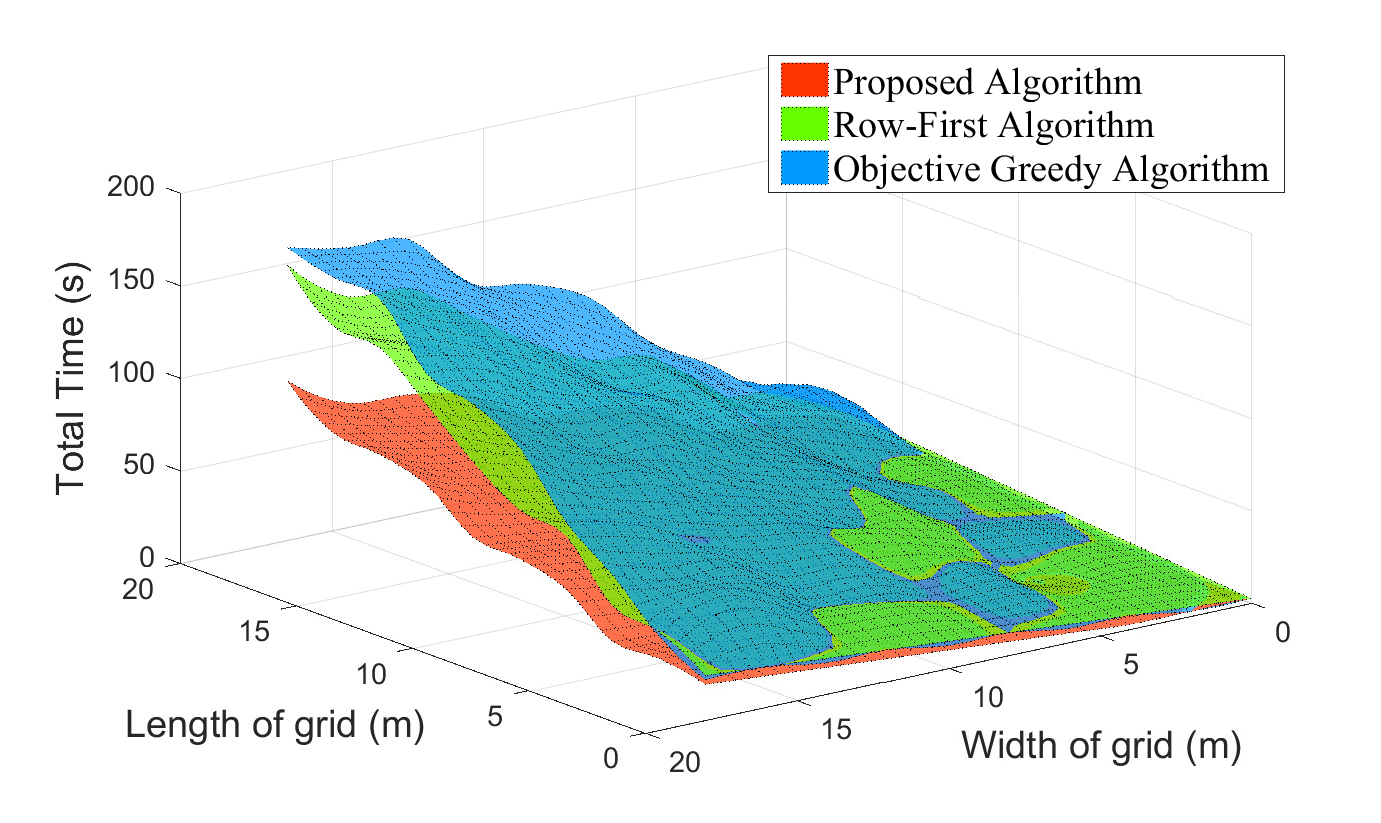
\includegraphics[width=0.7\linewidth]{pix/sensing-traj/eva_grid_time.pdf}
\caption{Comparison of the proposed, row-wise, and greedy algorithms on time consumed in different-size grids.}
\vspace{-0.15in}
\label{fig:eva_grid_time}
\end{figure}
%\section{Acknowledgements}
%
%This work was partially supported by National Natural Science Foundation
%of China under grant number 61201245, Specialized Research Fund for the Doctoral Program of Higher Education (SRFDP) under grant 20120001120128, and by the National Science Foundation through grants CNS-1314598 and IIP-1265886.

\bibliographystyle{IEEEbib}
\small
\bibliography{Sensing-traj}
\end{document}
